\documentclass[twoside,english]{uiofysmaster}
\usepackage[T1]{fontenc} %for å bruke æøå
\usepackage[utf8]{inputenc}
\usepackage{amsmath, amsfonts, amssymb}
\usepackage{graphicx} %for å inkludere grafikk
\usepackage{verbatim} %for å inkludere filer med tegn LaTeX ikke liker
\usepackage[font=scriptsize]{caption}
\usepackage{subcaption}
\usepackage{mdwlist}
\usepackage[toc,page]{appendix}
\usepackage{bm}
\usepackage{enumerate}
\usepackage{mathtools}
\usepackage{booktabs} 
\usepackage{hyperref}


\newcommand*\diff{\mathop{}\!\mathrm{d}}
\def\mbf#1{\mathbf{#1}}
\newcommand{\VV}{\mathbf{V}}
\newcommand{\Vv}{\mathbf{v}}
\newcommand{\VX}{\mathbf{X}}
\newcommand{\Vx}{\mathbf{x}}
\newcommand{\VH}{\mathbf{H}}
\newcommand{\Vh}{\mathbf{h}}
\newcommand{\VW}{\mathbf{W}}
\newcommand{\Vwi}{\mathbf{w}_{i*}}
\newcommand{\Vwj}{\mathbf{w}_{*j}}
\newcommand{\Va}{\mathbf{a}}
\newcommand{\Vb}{\mathbf{b}}

\usepackage{caption}
\captionsetup[figure]{font=normalsize}
\captionsetup[table]{font=normalsize}

\newcommand{\ra}[1]{\renewcommand{\arraystretch}{#1}}


\newcommand*\dif{\mathop{}\!\mathrm{d}}
\DeclarePairedDelimiter{\norm}{\lVert}{\rVert}

\bibliographystyle{ieeetr}
%\bibliography{references}

\author{Vilde Moe Flugsrud}
\title{Solving Quantum Mechanical Problems with Machine Learning}
\date{June 2018}

\begin{document}

\maketitle

\begin{abstract}
This is an abstract text.
\end{abstract}

\begin{acknowledgements}
I would like to thank Morten Hjort-Jensen for being an inspiring and helpful supervisor. Thank you for including me in your adventurous research spirit - I think I will remember one of your comments when considering this project for a long time "It will be a bit like throwing yourself into deep water. Personally, I love that."

I want to thank computational physics and Anders Malthe-Sørensen, who provided me and others with exciting summer research projects as first years students and subsequently allowed us to have an office space in your group. I want to thank my office (the Ministry of Silly Imports) mates of four years, Magnus, Alocias and Øyvind. It feels like we have grown up together, from wide-eyed second-year bachelor students to multiple degree- and job-juggling master students. I am lucky to have been around your knowledge, intelligence, enthusiasm, humor and warmth during this time.

I want to thank "FAMinistene" for being such good friends these past five years, demonstrating that a physics degree should not be feared for the lack of excellent girlfriends. Thank you for dinner nights, concerts, trips abroad, evenings at Realistforeningen, coffees at Deilig and Georg and so much more. I hope that some of these traditions will be kept even as we leave Blindern and that new ones will be created. Thank you Helene and Elisabeth for finding as much joy in Llamas as me - this is meant to summarize a lot more than meets the eye. Thank you Ingrid for your never-ending capacity for fun experiences, lots of humor and intense discussions be it about life or physics.

Thank you Sebastian for filling these past few years with memories worth a life-time, be it road tripping in Western Australia, crossing the Mediterranean Sea or climbing blue mountains, to mention a few. Thank you for all your love and support.

Finally, I would like to thank my family in general and in particular my mom, dad and brother Marius for always being there. 
\end{acknowledgements}

\tableofcontents

\chapter{Introduction}

Start your chapter by writing something smart. Then go get coffee.

\part{Theory}

\chapter{The Quantum Many-Body Problem}

\section{Many-Body Quantum Mechanics}
Quantum mechanics describes systems at the size of atoms and subatomic particles at speeds where relativistic effects are negligible. While in classical mechanics the state of a system of $N$ particles is given by each particle's position and momentum, in quantum mechanics it is determined by the complex valued wavefunction $\Psi$, which is an element of an infinite dimensional Hilbert space. That is, a complete vector space with an inner product.\cite{Kvaal2017}

Given a system's wavefunction we can calculate all physical quantities of interest\cite{Kvaal2017}. We call them observables and in quantum mechanics they are represented by hermitian operators.
The expectation value of an operator $\hat{\bm{O}}$ for a system of $N$ particles is given as \cite{HjortJensen2015}
\begin{align}
	%\langle \hat{\bm{O}} \rangle
	\langle \hat{\bm{O}} \rangle =& \frac{\int \Psi^{\ast}(\bm{x}_1,...,\bm{x}_N) \hat{\bm{O}}(\bm{x}_1,...,\bm{x}_N)
	\Psi (\bm{x}_1,...,\bm{x}_N)
	\dif \bm{x}_1 ... \dif \bm{x}_N  }
	{\int \Psi^{\ast}(\bm{x}_1,...,\bm{x}_N)
	\Psi (\bm{x}_1,...,\bm{x}_N)
	\dif \bm{x}_1 ... \dif \bm{x}_N}
\end{align}

For a system of $N$ particles in 3 spatial dimensions we see that this becomes a $3N$-dimensional integral. Furthermore, in order to compute it, we first need to have $\Psi$. This requires us (if we are interested in the ground state energy fex - see nuclear book) to solve the time-independent Schrödinger equation
\begin{align}
	\hat{\bm{H}} \Psi =& E\Psi .
\end{align}
For a complicated many body problem this can turn out to be a problem consisting of millions of coupled second-order differential equations in $3N$ dimensions.

To do:
\begin{itemize}
	\item Spin
	\item The postulates?
\end{itemize}

\section{Approximating wave functions}
Some selected conditions $\Psi$ must satisfy \cite{HjortJensen2015} are normalization 
\begin{align}
	\int_{-\infty}^{\infty} P(x,t) \dif x = \int_{-\infty}^{\infty} \Psi^{\ast}(x,t) \Psi (x,t) \dif x = 1
\end{align}
and that $\Psi (x,t)$ and $\partial \Psi(x,t) / \partial x$ must be finite, continuous and single valued.

Furthermore we have that \cite{Helgaker2000} (for molecular electroic-structure systems)
\begin{enumerate}
	\item The approximate state should be an eigenfunction of the number operator.
	\item The exact wavefunction is antisymmetric with respect to the permutation of any pair of electrons.
	\item For a bound state, the exact wave function is square-integrable and hence normalizable.
	\item The exact wavefunction is variational in the sense that, for all possible variations $\delta \Psi$ that are orthogonal to the wavefunction, the energy is stable (More in: Epstein's The Variation Method in Quantum Chemistry).
	\item The exact wavefunction is size-extensive. 
	\item In non-relativistic theory, the exact stationary states are eigenfunctions of the total and projected spin operators.
	\item Within the Born-Oppenheimer approximation, the exact stationary states form a basis for an irreducible representation of the molecular point group. 
	\item Owing to the presence of the Couloumb potential, the molecular electronic Hamiltonian becomes singular when two electrons coincide in space.
	\item Asymptotic behavior at large distances from the molecule
	\item Changes in a characteristic way under gauge transformations of the potentials associated with electromagnetic fields.
\end{enumerate}


Evt also requirements from \cite{Ledum2017}

\section{Quantum many body methods}
Brief overview over popular methods.

Summary from \cite{Ledum2017}
\begin{itemize}
	\item In practice, most methods are limited to systems of containing on the order of between $10^2$ (for high- precision methods such as con guration interaction, coupled cluster, di usion Monte Carlo, etc.) and $10^5$ electrons (for faster Hartree-Fock and density functional methods).
	\cite{Hu2015} \cite{VandeVondele2012} \cite{Bowler2010}
	\item As previously noted, solving the Schrodinger equation (SE) exactly by hand is impos- sible in the overwhelming majority of interesting cases. However, methods which can get close to the exact solution exists. Full Configuration Interaction (FCI) or direct diagonalization of the Hamiltonian is exact in the limit of an in nite orbital basis set but suffers from an exponential complexity scaling (in system and basis size). \cite{Helgaker2000}
	\item The related Confguration Interaction (CI) and Coupled Cluster (CC) approaches both truncate the FCI expansion of Slater determinants, thus gaining speed but loosing some accuracy. \cite{Kvaal2017} \cite{Hammond1994}
	\item Diffusion Monte Carlo (DMC) techniques can in principle provide the exact solution to the SE by imaginary-time evolution of an initial wave function guess. \cite{HjortJensen2015} \cite{Hammond1994}
	\item In practice, DMC methods are highly dependent on this ansatz and thus require as input the results of less accurate method but faster methods. One example may be the Variational Monte Carlo (VMC) method: conceptually simpler and faster than DMC, but not as accurate
	\cite{Hammond1994}
	\item The Hartree-Fock (HF) framework—which provides an e cient but not enormously accurate result—has seen extensive use since its inception in 1930
	\begin{itemize}
		\item D. R. Hartree. “The Wave Mechanics of an Atom with a Non-Coulomb Central Field. Part I. Theory and Methods”. In: Mathematical Proceedings of the Cam- bridge Philosophical Society 24.1 (1928), pp. 89–110. doi: 10.1017/S0305004100011919.
		\item V. Fock. %“Näherungsmethode zur Lösung des quantenmechanischen Mehrkör- perproblems”. In: Zeitschrift für Physik 61.1 (Jan. 1930), pp. 126–148. issn: 0044-3328. doi: 10.1007/BF01340294. url: https://doi.org/10.1007/BF01340294.
		\item A. Szabo and N.S. Ostlund. Modern Quantum Chemistry. Dover Publications, 1996. isbn: 0-486-69186-1.
	\end{itemize}
	\item However, by far the most popular approximation is Density Functional Theory (DFT), devel- oped by W. Kohn and L. J. Sham in 1965
	\begin{itemize}
		\item W. Kohn and L. J. Sham. “Self-Consistent Equations Including Exchange and Correlation E ects”. In: Phys. Rev. 140 (4A Nov. 1965), A1133–A1138. doi: 10. 1103/PhysRev.140.A1133. url: https://link.aps.org/doi/10.1103/PhysRev.140. A1133.
		\item R.M. Martin. Electronic Structure. Cambridge University Press, 2004. isbn: 0- 521-53440-2.
	\end{itemize}
	Between 1980 and 2010, DFT was the most active  eld in physics with eight out of the top ten most cited papers being on the subject 
	\begin{itemize}
		\item Axel D. Becke. “Perspective: Fifty years of density-functional theory in chem- ical physics”. In: The Journal of Chemical Physics 140.18 (2014), 18A301. doi: 10.1063/1.4869598. eprint: https://doi.org/10.1063/1.4869598. url: https: //doi.org/10.1063/1.4869598.
	\end{itemize}
	\item Computational scaling of \textit{ab initio} QM models range from $\mathcal{O}(N!)$ in the extreme (FCI) via $\mathcal{O}(N^6)$ (CC with singles, doubles, and estimated connected triples) and $\mathcal{O}(N^4)$ (formal HF), to $\mathcal{O}(N^3)$ for Hatree-Fock with integral pre-screening and density fitting.
	\begin{itemize}
		\item Laura E. Ratcli  et al. “Challenges in large scale quantum mechanical calculations”. In: Wiley Interdisciplinary Reviews: Computational Molecular Science 7.1 (2017). e1290, e1290–n/a. issn: 1759-0884. doi: 10.1002/wcms.1290. url: http://dx.doi.org/10.1002/wcms.1290.
	\end{itemize}
\end{itemize}


\section{Variational Monte Carlo}
\subsection{The Variational Principle}
Two theorems stated in \cite{Kvaal2017}, \cite{Helgaker2000}.
Simple formulation:
Given a \textit{trial state} $| \Psi_T \rangle$, the following inequality holds:
\begin{align}
	E_T = \frac{ \langle \Psi_T | \hat{H} | \Psi_T \rangle }{ \langle \Psi_T |\Psi_T \rangle } \geq E_0
\end{align}
where $E_0$ is the ground state eigenvalue of the Hamiltonian $\hat{H}$, and $E_T$ is the trial eigenvalue. The variational principle holds for the ground state, but also for excited states, provided that $|\Psi_T \rangle$ is orthogonal to all the eigenstates having eigenvalue lower than that of the state one wants to approximate.
\cite{HjortJensen2017}

\subsection{Monte Carlo Integration}
\subsubsection{Introductory statistics and probability}

For a continuous random variable $X$ distributed according to the probability density $p(X)$ the $n$th \textbf{moment} of $X$ is defined as
\begin{align}
	\langle X^n \rangle = \int p(x) x^n \dif x ,
\end{align}
where we notice that the zeroth moment recovers the \textbf{normalization condition} of the total probability,
\begin{align}
	1 = \int p(x) \dif x ,
\end{align}
and the first moment recovers the definition of the \textbf{expectation value} of $X$, 
\begin{align}
	\mu = E(X) = \langle X \rangle = \int p(x) x \dif x .
\end{align}


Furthermore we have that the \textbf{central moments} of $X$ are defined
\begin{align}
	\langle (X-\mu)^n \rangle = \int p(x) (x - \mu)^n \dif x .
\end{align}

Of particular interest here is the second central moment, which is what we know as the \textbf{variance} of $X$
\begin{align}
	\sigma^2 = var(X) = \langle (X-\mu)^2 \rangle =& \int p(x) (x - \mu)^2 \dif x  \\
	=& \int p(x) (x^2 - 2x \langle X \rangle + \langle X \rangle^2) \dif x \\
	=& \langle X^2 \rangle - 2\langle X \rangle \langle X \rangle + \langle X \rangle^2  \\
	=& \langle X^2 \rangle - \langle X \rangle^2
\end{align}
The square root of the variance, $\sigma$, is called the \textbf{standard deviation} or \textbf{standard error}. 

For two random variables $X$ and $Y$ we have that the expectation of a linear combination of them is equal to a linear combination of their expectations, $E(\lambda_1 X + \lambda_2 Y) = \lambda_1 E(X) + \lambda_2 E(Y)$. This is true whether $X$ and $Y$ are dependent or independent. In the variance however we see a difference between these two cases. We have in general that
\begin{align}
	var(\lambda_1 X + \lambda_2 Y) =& \lambda_1^2 var(X) + \lambda_2^2 var(Y) + 2 \lambda_1 \lambda_2 ( \langle XY \rangle
	- \langle X \rangle \langle Y \rangle) \\
	=& \lambda_1^2 var(X) + \lambda_2^2 var(Y) + 2 \lambda_1 \lambda_2 cov (X, Y)
\end{align}
The \textbf{covariance} $cov(X, Y) = \langle XY \rangle	- \langle X \rangle \langle Y \rangle$ measures the degree of independence between the two random variables. This is related to the probability of independent random events. If the two random variables are \textbf{independent}, we have that their joint probability can be written as a product of their respective probability distributions,
\begin{align}
	p(X, Y) = p(X) p(Y) .
\end{align}
Hence the expectation of the product $XY$ is
\begin{align}
	\langle XY \rangle = \int p(x, y) xy \dif x \dif y = \int p(x) x \dif x \int p(y) y \dif y
	=\langle X \rangle \langle Y \rangle
\end{align}
We see from this that if the two random variables are independent, $cov(X,Y) = 0$. Zero covariance by itself does not, however, guarantee independence.

From the covariance we may derive the \textbf{correlation coefficient}
\begin{align}
	\rho(X,Y) =& \frac{cov(X,Y)}{\sqrt{ \langle X \rangle \langle Y \rangle }}, \quad
	-1 \geq \rho(X,Y) \leq 1
\end{align}

Given the \textbf{bivariate probability distribution function} $p(X,Y)$ of two random variables, the \textbf{marginal probability distribution function} can be found for either of the them by 
\begin{align}
	p(X) = \int p(X,y) \dif y
\end{align}
The \textbf{conditional probability} is then given
\begin{align}
	p(Y|X) = \frac{p(X,Y)}{p(X)}
\end{align}
This can be generalized to multivariate distributions of more than two random variables.


\subsubsection{Estimators}
Suppose the variables $X_1, X_2,...$ are drawn randomly, but not necessarily independently, from the probability distribution function $p(X)$. Let $g$ be a function of $X$ and define the function $G_N$ by
\begin{align}
	G_N = \frac{1}{N} \sum_{i=1}^N g(x_i)
\end{align}
The expected value of $G_N$ is then
\begin{align}
	\langle G_N \rangle = \langle \frac{1}{N} \sum_i^N g(X_i) \rangle = \frac{1}{N} \sum_i^N \langle g(X) \rangle = \langle g(X) \rangle
\end{align} 
$G_N$ is the arithmetic average of the samples $g(X_i)$ and has the same expectation value as $g(X)$. $G_N$ is said to be an \textbf{estimator} of $\langle g(X) \rangle$. 

If all the $X_i$ are independent, the variance of $G_N$ is
\begin{align}
	var(G) = var( \frac{1}{N} \sum_i^N g(X_i)  ) = \sum_i^N \frac{1}{N^2} var(g(X)) 
	= \frac{1}{N} var(g(X))
\end{align}

The implication of this is that as the number of samples of $X$, $N$, increases, the variance of the mean value of $G_N$ decreases as $\frac{1}{N}$. This is a core idea of Monte Carlo integration. That is, since we may estimate an integral with a sum
\begin{align}
	\langle g(X) \rangle = \int_{-\infty}^\infty p(x) g(x) \dif x = \langle \frac{1}{N} \sum_{i=1}^N g(X_i) \rangle,
\end{align}

The next question is then, how does the sample average $G_N$ approach the expected value as $N$ increases?


\subsubsection{Convergence}
We here present three results about the estimator $G_N$.

\begin{enumerate}
\item \textbf{The Law of Large Numbers}: Suppose we have independent, identically distributed (i.i.d.) random variables $X_1,...,X_N$. The expectation of each $X$ is then $\mu$. As $N\rightarrow \infty$, the mean value of the $\{ X_i \}$, 
\begin{align}
	\bar{X}_N = \frac{1}{N} \sum_{i=1}^N X_i
\end{align}
is \textit{almost sure to converge} to $\mu$, meaning
\begin{align}
	p(\lim_{N\to \infty} \bar{X_N} = \mu) = 1 .
\end{align}

\item \textbf{The Chebychev Inequality}:
To estimate the \textit{speed} of convergence we must make stronger assumptions. We assume an estimator $G_N$, its mean $\langle G_N \rangle$ and variance $var(G_N)$ all exist. The Chebychev inequality then is
\begin{align}
	p\bigg (|G_N - \langle G_N \rangle | \geq \sqrt{\frac{var(G_N)}{\delta}} = \sqrt{\frac{var(g)}{\delta N}} \bigg ) \leq \delta 
\end{align}
with $\delta$ any postive number. By making $N$ big, we can make the variance of $G_N$ as small as we want, and the probability of the estimate differing from the true value by a large deviation relative to $\delta$ becomes small. This is at the core of the Monte Carlo method for evaluating integrals.

\item \textbf{The Central Limit Theorem}:
This theorem makes a much stronger statement about the possible values of $G_N$ than the Chebychev inequality. For any fixed value of $N$, the values of $G_N$ are described by some probability distribution function. The central limit theorem shows that as $N\rightarrow \infty$ there is a specific limit distribution. That is, the \textbf{normal distribution}, specified by
\begin{align}
	p(G_N) = \frac{1}{\sqrt{2\pi \cdot var(G_N)}} e^\frac{( G_N - \langle G_N \rangle )^2 }{2 \cdot var(G_N)}
	= \frac{1}{\sqrt{2\pi \frac{\sigma^2}{N} }} e^{\frac{N(G_N - \langle g\rangle)^2}{2\sigma^2}}
\end{align}
where $\sigma^2 = var(g)$. 
As $N\rightarrow \infty$ the values of $G_N$ occurs ever closer to $\langle g \rangle$. Given the standard deviation $\sigma/\sqrt{N}$, we have that the values of $G_N$ are within one standard deviation 68.3\% of the time, within two standard deviations 95.4\% of the time, and within three standard deviations 99.7\% of the time.
The central limit theorem is very powerful in that it gives a specific distribution for the values of $G_N$, but it applies only asymptotically. How large $N$ must be before the central limit theorem applies depends on the problem.

\end{enumerate}

Without the central limit theorem, there is in general only the much weaker upper bound of the Chebychev inequality to suggest how much the observed $G_N$ deviates from the actual mean. Of course, in specific cases, studies can be made of the distribution of the estimator. Much Monte Carlo is done assuming that the theorem has been satisfied no matter what the sample size; reported errors must be considered optimistic in such cases.


We may estimate the variance $\sigma^2 = var(g(x))$ using independent values of $g(x_i)$ by
\begin{align}
	s^2 = \frac{1}{1-N} \sum_i^N (g(X_i) - G_N)^2 = \frac{N}{N-1} (  \frac{1}{N} \sum_{i=1}^N g^2(X_i) - G_N^2  )
\end{align}
where we have that $E(s^2) = \sigma^2 $, which means that $s^2$ is an unbiased estimate of $\sigma^2$. From this we also have an estimator of the variance of the estimated mean
\begin{align}
	var(G_N) = \frac{1}{N} \sigma^2 \approx \frac{1}{N} s^2
\end{align}
From these we may also estimate the standard deviation as $\sigma \approx s$ and $std(G_N) \approx s/\sqrt{N}$ respectively. While $E(s^2) = \sigma^2$ it does not imply $E(s) = \sigma$, hence $s$ is not an unbiased estimate of $\sigma$. However it is a good approximation when the sample size $N$ is large.

Also mention:
Note that we can do integrations in multiple dimensions with suprisingly little loss of computational efficiency. That one can work in many dimensions – indeed one can add extra dimensions – is a characteristic of Monte Carlo quadrature in contrast to discrete numerical quadrature, and is a property that can be exploited to great advantage in many applications.


Pseudorandom numbers might be wanted over truly random numbers for several reasons where one is dependent on being able to recreate program runs.

\subsubsection{Importance Sampling}



\subsubsection{Local Energy}

How do we relate the quantum mechanical energy to a Monte Carlo estimator? We have that \cite{Toulouse2016}
\begin{align}
	E_v =& \frac{\langle \Psi | \hat{H} | \Psi \rangle}{\langle \Psi | \Psi \rangle}  \\
	=& \frac{ \int \Psi^\ast (\bm{R}) \hat{H} \Psi(\bm{R}) \dif \bm{R} }
	{\int \Psi^\ast \Psi(\bm{R}) \dif \bm{R}} \\
	=& \frac{ \int \Psi^\ast (\bm{R}) (\Psi(\bm{R}) \frac{1}{\Psi(\bm{R})}) \hat{H} \Psi(\bm{R}) \dif \bm{R} }
	{\int | \Psi(\bm{R})|^2 \dif \bm{R}} \\
	=&  \frac{ \int \Psi^\ast (\bm{R}) \Psi(\bm{R}) \frac{\hat{H} \Psi(\bm{R}) }{\Psi(\bm{R})}  \dif \bm{R} }
	{\int | \Psi(\bm{R})|^2 \dif \bm{R}} \\
	=&  \frac{ \int | \Psi(\bm{R})|^2  E_L(\bm{R})  \dif \bm{R} }
	{\int | \Psi(\bm{R})|^2 \dif \bm{R}} \\
	=& \int P(\bm{R}) E_L (\bm{R}) \dif \bm{R}
\end{align}

where the local energy is defined $E_L = \frac{\hat{H} \Psi(\bm{R}) }{\Psi(\bm{R})} $ and $P(x) = \frac{| \Psi(\bm{R})|^2 }{ \int | \Psi(\bm{R})|^2 \dif \bm{R} }$ is the normalized probability given by the squared absolute wave function. 

We then recognize that we can use as our Monte Carlo \textit{estimator} the quantity
\begin{align}
	\frac{1}{N} \sum_{i=1}^N E_L(\bm{R}_i)
\end{align}
with $\bm{R_i}$ sampled from $P(\bm{R})$ to approximate, as $N \rightarrow \infty$, 
\begin{align}
	\langle \frac{1}{N} \sum_{i=1}^N E_L(\bm{R}_i) \rangle = \int P(\bm{R}) E_L(\bm{R}) \dif \bm{R} = E_v
\end{align}

Toulouse et al. \cite{Toulouse2016} gives the definition of local energy as: The expectation value of an operator $\hat{O}$ can be computed by averaging the corresponding local value
\begin{align}
	O(\bm{R}_f) = \frac{ \langle \bm{R}_f | \hat{O} |\Psi \rangle }{ \langle \bm{R}_f | \Psi \rangle }
\end{align}
at the Monte Carlo points $\bm{R}_f$ after the accept/reject step.

Umrigar \cite{Umrigar1999} defines $E_L$, or generally a \textbf{configurational eigenvalue} $X (\bm{R})$ as
\begin{align}
	X(\bm{R}) \Psi(\bm{R}) = \langle \bm{R} | \hat{X} | \Psi(\bm{R}) \rangle
	 = \sum_{\bm{R}'} \langle \bm{R} | \hat{X} | \bm{R}' \rangle \langle \bm{R}' | \Psi \rangle
\end{align}

More on how we need the local energy because we need operators that are diagnoal/near diagonal in the used basis in 
\cite{Umrigar1999} and Carleo seminar notes.






\subsection{Markov Chains}
\label{sec:MarkovChains}

Monte Carlo integration requires us to sample from the probability distribution of interest. However we are not able to do this directly when the normalization constant is intractable. We turn instead to Markov chains. A Markov chain is a type of Markov process, which is a type of stochastic process. A \textbf{stochastic process} is a stochastic quantity $Y$ that can be mapped from a stochastic variable $X$ with a function $f$, and that also depends on another "normal" variable $t$, which usually represents time. That is,
\begin{align}
	Y_X (t) = f(X,t)
\end{align}


The probability density for $Y_X(t)$ to take any value $y$ at time $t$ is then
\begin{align}
	P_1 (y, t) = \int \delta (y- Y_X (t)) P_X (x) \dif x
\end{align}
Similarly the joint probability density that $Y$ has the value $y_1$ at $t_1$, and also $y_2$ at $t_2$ and so on till $y_n$ at $t_n$ is
\begin{align}
	P_n (y_1, y_1; y_2, t_2; ...; y_n, t_n)
	= \int \delta (y_1 - Y_x (t_1)) ... \delta (y_n - Y_x (t_n)) P_x (x) \dif x
\end{align}
In this way a hierarchy of probability densities $P_n (n=1,2,...)$ is defined.
Considering $P_n$ to be defined only when all times are different, the hierarchy of functions $P_n$ then obeys the following four \textbf{consistency conditions}.
\begin{enumerate}
	\item $P_n \geq 0$
	\item $P_n$ does not change on interchanging two pairs $(y_k, t_k)$ and $(y_l, t_l)$
	\item $\int P_n (y_1, t_1; ...; y_n, t_n) \dif y_n = P_{n-1} (y_1, t_1; ...; y_{n-1}, t_{n-1}) $
	\item $\int P_1 (y_1, t_1) \dif y_1 = 1$ 
\end{enumerate}
Any set of functions that obey the four consistency conditions determines a stochastic process.


A \textbf{Markov process} is a stochastic process that has the \textbf{Markov property}. The Markov property is that the next state is dependent only on the current state, and no more history than that. It is that for any set of $n$ successive times (i.e. $t_1<t_2<t_3$) one has
\begin{align}
	P_{1|n-1} (y_n, t_n | y_1, t_1; ...; y_{n-1}, t_{n-1}) = P_{1|1} (y_n, t_n | y_{n-1}, t_{n-1})
\end{align}
Meaning, the conditional probability density at $t_n$, given the value $y_{n-1}$ at $t_{n-1}$, is uniquely determined and not affected by any knowledge of the values at earlier times. $P_{1|1}$ is then known as the \textbf{transition probability}.

A Markov Process then is fully determined by the two functions:
\begin{enumerate}
	\item The initial probability distribution: $P_1 (y_1, t_1)$
	\item The transition probability: $P_{1|1} (y_2, t_2| y_1, t_1)$ 
\end{enumerate}
From this one can use the definition of conditional probability to successively construct all $P_n$. The two functions $P_1$ and $P_{1|1}$ cannot be chosen arbitrarily, but have to obey
\begin{enumerate}
	\item The Chapman-Kolmogorov equation 
	\item $P_1(y_2, t_2) = \int P_{1|1} (y_2, t_2| y_1, t_1) P_1 (y_1, t_1) \dif y_1$
\end{enumerate}
where the \textbf{Chapman-Kolmogorov equation} is, given $t_1 < t_2 < t_3$, the identity
\begin{align}
	P_{1|1} (y_3, t_3| y_1, t_1) = \int P_{1|1} (y_3, t_3|y_2, t_2) P_{1|1} (y_2, t_2 | y_1, t_1) \dif y_2
\end{align}

Any two non-negative functions $P_1$ and $P_{1|1}$ that obey these consistency conditions uniquely determines a Markov Process.

A stochastic process in general is said to be \textbf{stationary} when the moments are not affected by a shift in time, that is
\begin{align}
	\langle Y(t_1 + \tau)...Y(t_n + \tau) \rangle = \langle Y(t_1 )...Y(t_n ) \rangle
\end{align}
for all $n$, all $\tau$, and all $t_1, ..., t_n$.

For a \textbf{stationary Markov process} then we have that the transition probability $P_{1|1}$ does not depend on two times but only on the time interval; we introduce the notation
\begin{align}
	P_{1|1} (y_2, t_2| y_1, t_1) = T_\tau (y_2|y_1), \quad \tau = t_2 - t_1
\end{align}

The Chapman-Kolmogorov equation then becomes $(\tau, \tau' > 0)$
\begin{align}
	T_{\tau+\tau'} (y_3 | y_2) = \int T_{\tau'} (y_3|y_2) T_\tau (y_2|y_1) \dif y_2
\end{align}
If we read the integral as a product of two matrices, or integral kernels, this may be written
\begin{align}
	T_{\tau + \tau'} = T_{\tau'} T_{\tau}, \quad (\tau, \tau' > 0)
\end{align}


We may now define \textbf{Markov chains}. These are an especially simple class of Markov processes, defined by the properties
\begin{enumerate}
	\item The range of $Y$ is a discrete set of states
	\item The time variable is discrete and take only integer values $t=...,-2,-1,0,1,2,...$
	\item The process is stationary, so the transition probability depends on the time difference alone.
\end{enumerate}
A \textbf{finite Markov chain} has a range consisting of a finite number $N$ states. 

Thus, we have that
\begin{itemize}
	\item The initial probability distribution $P_1 (y, t)$ is an $N$-component vector $p_n(t)$ ($n=1,2,...,N$).
	\item The transition probability $T_\tau (y_2|y_1)$ is an $N\times N$ matrix.
\end{itemize}

The Markov property then leads to the equation
\begin{align}
	T_\tau = (T_1)^{\tau} (\tau = 0,1,2,...)
\end{align}
The probability distribution $p(t)$ originating from the initial distribution $p(0)$ is, in matrix notation,
\begin{align}
	p(t) = T^t p(0)
\end{align}
The study of finite Markov chains amounts to investigating the powers of an $N\times N$ matrix $T$ of which we only know that it is a \textbf{stochastic matrix}. That is,
\begin{enumerate}
	\item Its elements are non-negative.
	\item Each column adds up to unity.
\end{enumerate}
It is clear that $T$ has a left eigenvector $(1,1,...,1)$ with eigenvalue 1, and therefore a right eigenvector $p^s$ such that $T p^s = p^s$, which is the $P_1(y)$ of the stochastic process.
The prinicpal task of the theory then is to show that for any initial $p(0)$
\begin{align}
	\text{lim}_{t\rightarrow \infty} p(t) = \text{lim}_{t\rightarrow \infty} T^t p(0) = p^s
\end{align}
(and this has been shown by so and so except for a few exceptional cases?)
\cite{VanKampen2007}




\subsection{Metropolis-Hastings Algorithm}
\label{sec:MetroHastings}

How do we use Markov Chains to sample from $P(\bm{R})$ then?

\subsubsection{Ergodicity}
The point of using Markov Chains is to be able to sample our desired distribution $P(\bm{R})$. We start from an arbitrary initial state $\bm{R}_i$ and evolve the system by repeated application of a Markov transition matrix $T$. The stationary property, which implies that
\begin{align}
	\sum_i T(\bm{R}_f | \bm{R}_i) P (\bm{R}_i) = \sum_i T (\bm{R}_i | \bm{R}_f) P (\bm{R}_f) = P(\bm{R}_f)
\end{align}
(where we used that $P$ is an eigenvector of $T$ with eigenvalue 1), and ensures that if we start with the desired distribution $P$, we will continue to sample from that same distribution.

However, we want that \textit{any} initial distribution should evolve to the desired distribution $P$ under the repeated application of $T$, i.e., $lim_{n\rightarrow \infty} M^n (\bm{R}' | \bm{R}) = \rho(\bm{R}')$, independent of $\bm{R}$. 

Aka, not only should $\rho$ be a right eigenvector of $M$ but it should be the \textit{dominant} right eigenvector. Necessary conditions are that transitions can be made with non-zero prob between (almost, ref) any pair of states in a finite number of steps and that $M$ not be cyclic. Such a matrix is \textbf{ergodic}. 
\cite{Umrigar1999}

\subsubsection{Detailed balance condition}
We have shown so far that we can sample $\rho$ by repeated application of a Markov matrix that satisfies the stationary condition, but we have not shown how such matrices are constructed in practice. In order to do this, the more stringent \textbf{detailed balance} condition
\begin{align}
	M(\bm{R}_f | \bm{R}_i ) \rho(\bm{R}_i) = M(\bm{R}_i | \bm{R}_f ) \rho(\bm{R}_f)
\end{align}
is usually imposed. 
It expresses the condition that for any pair of states $\bm{R}_i$ and $\bm{R}_f$ the rate of flow is the same in both directions. It is a sufficient, but not necessary, condition. Detailed balance implies the stationary condition, but the reverse is not true.
\cite{Umrigar1999}
A Markov chain satisfying the detailed balance condition is said to be \textbf{reversible}.\cite{Toulouse2016} 

In practice, a Markov chain is realized by a \textbf{random walk}. More in \cite{Toulouse2016} p. 293.

Starting from an initial point $\bm{R}_1$ (or walker) - i.e., a delta-function distribution $\delta (\bm{R} - \bm{R}_1)$ - sample the second point $\bm{R}_2$ by drawing from the probability distribution $P(\bm{R}_2|\bm{R}_1)$, then a third point $\bm{R}_3$ by drawing from $P(\bm{R}_3 | \bm{R}_2)$, and so on. After disregarding a certain number of iterations $M_{eq}$ corresponding to a transient phase called \textit{equilibration}, the random walk samples the stationary distribution $\rho(\bm{R})$ in the sense that
\begin{align}
	\rho(\bm{R}) = E[\delta (\bm{R} - \bm{R}_k) ] \approx \frac{1}{M} \sum_{k=1}^M \delta (\bm{R} - \bm{R}_k)
\end{align}
and the averages of the estimators of the observables of interest are calculated.

The rate of convergence to the stationary distribution $\rho(\bm{R})$ and the autocorrelation times of the observables are determined by the second largest eigenvalue of the matrix $P$ (see, e.g., Ref. \cite{Gilks1996}). The random walk must be sufficiently long so as to obtain a representative sample of states, making a nonnegligible contribution to the expected values. 
\cite{Toulouse2016}

\subsubsection{The Metropolis-Hastings Algorithm}
In the Metropolis-Hastings algorithm , one realizes a Markov chain with the following random walk. Starting from a point $\bm{R}_i$, a new point $\bm{R}_f$ is determined in two steps:
\begin{enumerate}
	\item A temporary point $\bm{R}_f'$ is proposed with the probability $P_{prop} (\bm{R}_f' | \bm{R}_i)$,
	\item The point $\bm{R}_f'$ is accepted (i.e., $\bm{R}_f = \bm{R}_f'$) with probability $P_{acc} (\bm{R}_f' | \bm{R}_i)$ or rejected (i.e., $\bm{R}_f = \bm{R}_i$) with probability $P_{rej}(\bm{R}_f' | \bm{R}_i) = 1 - P_{acc} (\bm{R}_f' | \bm{R}_i)$.
\end{enumerate}
The corresponding transition probability can be written as
\[ P(\bm{R}_f |\bm{R}_i ) = \begin{cases}
				P_{acc}(\bm{R}_f |\bm{R}_i ) P_{prop} (\bm{R}_f |\bm{R}_i )  
				& \quad \text{if} \bm{R}_f \neq \bm{R}_i \\
				1 - \int  P_{acc}(\bm{R}_f' |\bm{R}_i ) P_{propr} (\bm{R}_f' |\bm{R}_i )  \dif \bm{R}_f'
				& \quad \text{if} \bm{R}_f = \bm{R}_i  
\end{cases} \]
or, in a single expression,
\begin{align}
	P(\bm{R}_f |\bm{R}_i ) =& P_{acc}(\bm{R}_f |\bm{R}_i ) P_{prop} (\bm{R}_f |\bm{R}_i ) \\
	&+ [1-\int  P_{acc}(\bm{R}_f' |\bm{R}_i ) P_{propr} (\bm{R}_f' |\bm{R}_i )  \dif \bm{R}_f'] \delta(\bm{R}_i - \bm{R}_f)
\end{align}

The proposal probability $P_{prob}(\bm{R}_f |\bm{R}_i )$ is a stochastic matrix, i.e.
\begin{align}
	P_{prob}(\bm{R}_f |\bm{R}_i ) \geq 0 \quad \text{and} \quad
	\int P_{prob}(\bm{R}_f |\bm{R}_i ) \dif \bm{R}_f = 1,
\end{align}
ensuring that $P(\bm{R}_f| \bm{R}_i)$ fullfills the non-negativity condition. The second term with the delta function ensures that $P(\bm{R}_f| \bm{R}_i)$ fullfills the normalization condition. (Nonnegativity and column normalization then ensures $P(\bm{R}_f| \bm{R}_i)$ is a \textbf{stochastic matrix}).

The acceptance probability is chosen so as to fulfill the \textbf{detailed balance} condition,
\begin{align}
	P(\bm{R}_f| \bm{R}_i)  \rho (\bm{R}_i) = P(\bm{R}_i| \bm{R}_f) \rho (\bm{R}_f)
\end{align}

that is, for $\bm{R}_f \neq \bm{R}_i$,
\begin{align}
	\frac{ P_{acc} (\bm{R}_f| \bm{R}_i) }{ P_{acc} (\bm{R}_i| \bm{R}_f) }
	= \frac{ P_{prop} (\bm{R}_i| \bm{R}_f) \rho (\bm{R}_f) }
	{ P_{prop} (\bm{R}_f| \bm{R}_i) \rho (\bm{R}_i) }
\end{align}
Several choices are possible. The choice of Metropolis et al. \cite{Metropolis1953} maximizes the acceptance probability
\begin{align}
	P_{acc} (\bm{R}_f | \bm{R}_i) = \text{min} \{ 1, 
	\frac{ P_{prop} (\bm{R}_i| \bm{R}_f) \rho (\bm{R}_f) }
	{ P_{prop} (\bm{R}_f| \bm{R}_i) \rho (\bm{R}_i) } \}
\end{align}
The acceptance probability is not a stochastic matrix, even though both the proposal and the total Markov matrices are stochastic. Since only the ratio $\rho (\bm{R}_f)/\rho (\bm{R}_i)$ is involved in the above form of the accpetance probability, it is not necessary to calculate the normalization constaint of the probability density $\rho (\bm{R})$. It is clear that this acceptance probability is optimal, but there is a considerable scope for ingenuity in choosing a proposal probability $P_{prop} (\bm{R}_f| \bm{R}_i)$ that leads to a small autocorrelation time.

\cite{Toulouse2016}




\subsubsection{Importance sampling}
A simple, isotropic diffusion process characterized by a time-dependent density $f(\bm{x}, t)$ obey the following Fokker-Planck equation,
\begin{align}
	\frac{\partial f}{\partial t} = \sum_i D \frac{\partial}{\partial x_i} ( \frac{\partial}{\partial x_i} - F_i(\bm{x}) ) f .
\end{align}
Here $D$ is the diffusion constant and $F_i$ is the $i$-th component of a drift velocity $\bm{F}$ caused by an external potential. We wish to converge to the stationary density $f = \Psi^2 / \int \Psi^2 \dif \bm{x}$. An unchanging state, for which $\partial f / \partial t = 0$, may be obtained by setting the left-hand side of the above equation to zero, that is
\begin{align}
	\sum_i D(\frac{\partial^2 f}{\partial x_i^2} - \frac{\partial}{\partial x_i} (F_i f)  ) = 0
\end{align}
This equation is satisfied if each term of the sum vanishes, yielding
\begin{align}
	\frac{\partial^2 f}{\partial x_i^2} = f \frac{\partial}{\partial x_i} F_i + F_i \frac{\partial}{\partial x_i} f
\end{align}
The drift velocity $\bm{F}$ must therefore be of the form $F_i = g(f) \partial f/ \partial x_i$ in order to obtain a second derivatie of $f$ on the right hand side. Substituting this $\bm{F}$ into the previous equation gives us
\begin{align}
	\frac{\partial^2 f}{\partial x_i^2} = f \frac{\partial g}{\partial f} (\frac{\partial f}{\partial x_i})^2
	+ f g \frac{\partial^2 f}{\partial x_i^2} + g (\frac{\partial f}{\partial x_i})^2
\end{align}
For the second derivative terms to cancel we must have $g = 1/f$. This choice also leads to cancellation of the first derivative terms. Therefore the stationary density $f = \Psi^2 / \int \Psi^2 \dif \bm{x}$ results from choosing the drift vector to be
\begin{align}
	\bm{F} = \frac{1}{f} \nabla f = 2 \frac{1}{\Psi} \nabla \Psi
\end{align}
This drift causes the move to be biased by $\Psi$. This biased diffusion process incorporates importance sampling.



We now have a diffusion equation which gives the desired distribution, but how do we implement it using Monte Carlo? In statistical mechanics, Fokker-Planck trajectories are generated by means of a Langevin equation. The Langevin equation corresponding to the Fokker-Planck equation given above is 
\begin{align}
	\frac{\partial \bm{x} (t)}{\partial t} = D \bm{F} (\bm{x}(t)) + \eta
\end{align}
Here $\eta$ is a randomly fluctuating force which is distributed according to a multidimensional Gaussian with a mean of zero and a variance of $2D$. The Langevin equation arises from the theory of Brownian motion, closely related to diffusion. By integrating it over a short time interval, $\delta t$, we obtain a discretized form suitable for Monte Carlo simulation, which moves the particle from point $\bm{x}$ to $\bm{y}$ according to 
\begin{align}
	\bm{y} = \bm{x} + D \bm{F} (\bm{x}) \delta t + \chi
\end{align}
In this equation $\chi$ is a Gaussian random variable with a mean value of zero and a variance of $2D \delta t$. By using the discretized form rather than the continuous form, we have introduced a bias into the dynamics for any $\delta t \geq 0$. The distributed trajectories, and therefore the measured energy, will deviate increasingly from the exact as $\delta t$ increases. However, this error can be corrected by a Metropolis acceptance-rejection step.

We have that $G(\bm{y}, \bm{x}; \delta t)$ must be a solution of the Fokker-Planck equation with the added condition that $G(\bm{y}, \bm{x}; \delta t = 0) = \delta (\bm{x} - \bm{y})$. To solve the Fokker-Planck equation, it is convenient to rewrite it in the form, 
\begin{align}
	\frac{\partial f}{\partial t} = \mathcal{L} f,
\end{align}
where $\mathcal{L} = D \nabla \cdot (\nabla - \bm{F})$. Then $G(\bm{y}, \bm{x}; \delta t)$ is the spatial resolution of the operator $e^{-\mathcal{L} \delta t}$. In operator form, $G(\bm{y}, \bm{x}; \delta t)$ is given by 
\begin{align}
	G(\bm{y}, \bm{x}; \delta t)  = e^{ D \delta t ( \nabla^2 - \nabla \cdot \bm{F} - \bm{F} \cdot \nabla ) }
\end{align}
If we now assume that the force $\bm{F}$ remains essentially constant between $\bm{x}$ and $\bm{y}$, we can integrate the previous expression over a small time interval (which we will still call $\delta t$). This makes the expression a function of $\bm{x}$ and $\bm{y}$, which when normalized becomes
\begin{align}
	G(\bm{y}, \bm{x}; \delta t) = \frac{1}{(4 \pi D \delta t)^{\frac{3N}{2}}} e^{ - ( \bm{y} - \bm{x} - D\delta t \bm{F}(\bm{x}) )^2 / 4D \delta t }
\end{align}

Note that the update move found above is consistent with this expression, which is a Gaussian with variance $2D \delta t$ whose center is drifting due to a force vector field. Morover, this expression is a solution to the generalized diffusion equation givne before.

The function $G(\bm{y}, \bm{x}; \delta t)$  gives the probability of a walker moving from $\bm{x}$ to $\bm{y}$. Therefore the total density at point $\bm{y}$, i.e. the function $f(\bm{y})$, is given by the integral over all space of the transition probabilities multiplied by $f$ at each point, i.e. 
\begin{align}
	f(\bm{y} , t + \delta t) = \int G(\bm{y}, \bm{x}; \delta t)  f(\bm{x}, t) \dif \bm{x}
\end{align}
Repeated iterations of this expression by means of the given update move and the Metropolis acceptance step will therefore produce 
$f (\bm{y}, t \to \infty) = \Psi^2$ .

\cite{Hammond1994}

\subsection{Statistical errors and blocking}
The final estimate of the energy after Metropolis is given by $\langle E \rangle \pm \Delta E$ where:
\begin{align}
	\langle E \rangle =& \frac{1}{N_{steps}} E_{cumulative} \\
	\Delta E =& \sqrt{ \frac{1}{N_{steps}-1} ( \frac{1}{N_steps} E_{cumulative}^2 - \langle E \rangle^2 ) }
\end{align}

Summary from \cite{HjortJensen2017}:
\begin{itemize}
	\item Main hypothesis underlying the Central Limit Theorem: data used to construct the averages are sampled independently. Quite reasonable assumption in a measurement process.
	\item But: in the case of the computation of an integral by means of any method based on the Markov chain theory this requirement is not satisfied by construction. Data are sampled based on a transition matrix, and the resulting random walk has a certain degree of memory of the past events. Two consecutive samples will always be correlated to each other.
	\item But, we can hope that after a certain number of steps memory is lost, and data will become effectively independent. Is it possible to estimate this typical \textbf{correlation length}?
	\item Based on the previous argument one can define a measure of the autocorrelation by looking at the variance of the expectation of $F(X)$ (the function we want to integrate over to get the integral $I$) wrt $P(X)$:
	\begin{align}
		(\Delta I)^2 = \langle \frac{1}{N^2} \sum_{i=1}^N F(X_i) \sum_{i=1}^N F(X_j) \rangle - \langle F \rangle^2
	\end{align}
	\begin{itemize}
		\item (From where comes the motivation for the first term..? It seems very different from $\langle F^2 \rangle = \frac{1}{N} \sum_{i=1}^N F^2(X_i)$ which it is seemingly compared to by putting it there)
	\end{itemize}
	The corresponding standard deviation is the estimate of the statistical error on the integral of $F$. The first term can be recast in the following way:
	\begin{align}
		\langle \frac{1}{N^2} \sum_{i=1}^N F(X_i) \sum_{i=1}^N F(X_j) \rangle 
		=& \frac{1}{N^2} \sum_{i,j=1}^N \int P[X_1, ..., X_N] F(X_i) F(X_j) \dif X_1 ... \dif X_N \\
		=& \frac{1}{N^2} \sum_{i,j=1}^N \langle F(X_i) F(X_j) \rangle
	\end{align}
	Since the Markov chain is stationary, this quantity is expected to depend only on the difference of the indexes $\tau = i-j$. We will then define an \textbf{autocorrelation coefficient}:
	\begin{align}
		c(F)_\tau = \frac{\langle F(X_i) F(X_{i+\tau}) \rangle - \langle F \rangle^2}
		{ \langle F^2 \rangle - \langle  \rangle^2 }
	\end{align}
	\begin{itemize}
		\item Now $ \langle F^2 \rangle$ is being "compared" to  $\langle F(X_i) F(X_j) \rangle $ "instead", ie without the part $\frac{1}{N^2} \sum_{i,j=1}^N $. why?	
	\end{itemize}
	The coefficient is normalized to the variance $\sigma^2 (F)$, in such a way that $C(F)_0 = 1$.
	Correlation coefficients are related to the average of the product of the $F$ in the following way:
	\begin{align}
		\langle F(X_i) F(X_{i+\tau}) \rangle = c(F)_\tau \sigma^2 (F) + \langle F \rangle^2
	\end{align}
	we can use the previous expression to estimate the error on $I$:
	\begin{align}
		(\Delta I)^2 =& \frac{1}{N^2} \sum_{i,j=1}^N \langle F(X_i) F(X_j) \rangle - \langle F \rangle^2 \\
		=& \frac{1}{N} \sigma^2 (F) \sum_{\tau=1}^N c(F)_\tau + \langle F \rangle^2 - \langle F \rangle^2 \\
		=& \frac{\sigma^2 (F)}{N} \sum_{\tau=1}^N c(F)_\tau
	\end{align}
	As it can be seen \textbf{the error not only depends on the variance of} $F$, \textbf{but also on the sum over all the autocorrelation coefficients of} $F$. 
	\item This is the main consequence of having autocorrelated samples: the statistical error is underestimated by the variance of $F$, and needs to be corrected by a factor that depends on the autocorrelation length. 
	\item Usually the coefficients $c(F)_\tau$ have an exponential decay. If we approximate them as $c(F)_\tau \sim e^{-\frac{\tau}{\bar{\tau}}}$, the sum of the coefficients can be approximated as:
	\begin{align}
		\sum_{\tau=1}^N c(F)_\tau \sim \int_0^\infty \dif \tau e^{-\frac{\tau}{\bar{\tau}}} = \bar{\tau}
	\end{align}
	This means: It is sufficient to fit the exponential decay of the autocorrelation coefficients in order to find an estimate of the characteristic autocorrelation length that corrects the estimate of the error on the integral. In particular the correct expression for the error is:
	\begin{align}
		\Delta I \approx \sqrt{ \frac{1}{N-1} \sigma^2 (F) \bar{\tau} }
	\end{align}
	which has the simple interpretation: We are not generating $N$ independent samples of the variable $X$ during our Markov process, but rather $\frac{N}{\bar{\tau}}$ of them, and this number must be used as the correct count of events for the error estimation. 
	\item Important to be extremely careful about the estimation of autocorrelations. Underestimation of the statistical errors leads to a wrong interpretation of the results and to wrong physical conclusions.
	\item Autocorrelations also play a crucial role in choosing the step width $\Delta$ in the (simple) Metropolis-Hastings algorithm. A common criterion is to choose it in such a way that the fraction of accepted moves is about 50\%. However, the \textbf{ideal value is clearly the one minimizing the autocorrelations among samples}, and quite often this value corresponds to acceptances of the order 30 to 40\%. 
	\item Once the value of $\bar{\tau}$ has been estimated, it is possible to organize the calculation in such a way that the statistical error computed by the code is more realistic by using a \textbf{reblocking} technique. In practice the values of the quantity to be averaged are summed up in blocks of $N_b$ elements each:
	\begin{align}
		F_l^b = \sum_{i=1}^{N_b} F(X_i)
	\end{align}
	(Not divided by $N_b$...?) Then, the $F_l^b$ are used as the data on which performing the computation of the variance and of the standard deviation. If $N_b \gtrsim \bar{\tau}$, the standard deviation will be corrected by the effects of the autocorrelation of the original data. 
	\item Typically calculations store block values so that the values can be "reblocked" for example by combining pairs of blocks. The estimated error should be unchanged if the blocks are uncorrelated. In addition, the ratio of the block variance to the variance of the original function can be used to estimate the number of independent samples, and therefore the autocorrelation time.
\end{itemize}



\subsection{The Variational Monte Carlo Algorithm}


\section{The Quantum Dot System}
Quantum dots are systems of electrons tightly confined in a potential well. They have quantized energy levels and emit light in a fashion similar to atoms, hence they are sometimes referred to as artificial atoms. While the color of light emitted from atoms depend on the type of atom, the color emitted from quantum dots can be manipulated by controlling the size of the quantum dot. The possibility of controlling the properties of the quantum dot by fine-tuning its shape and size makes it attractive for several practical applications. Some include LEDs (Neidhardt et al 2015), solar cells (39), medical imaging (41) and acting as quantum bits (qbits) in quantum computers (42). (jorgen sources).

\subsection{Harmonic Oscillators}
For $P$ number of particles the Hamiltonian of a harmonic oscillator system is given 
\begin{align}
	\hat{\bm{H}} =& \sum_p^P (-\frac{1}{2} \nabla_p^2 + \frac{1}{2} \omega^2 r_p^2  ) ,
\end{align}
where natural units are used ($\hbar = c= e=m_e = 1$) and energies are in atomic units (a.u.). $r_p = \sqrt{x_p^2+y_p^2+z_p^2}$ is the position of electron $p$.

The wavefunctions for one electron in a harmonic oscillator potential in two and three dimensions are
\begin{align}
	\phi_{n_x, n_y} (\bm{r}) =& H_{n_x} (\sqrt{\omega}x) H_{n_y} (\sqrt{\omega}y) e^{-\frac{1}{2} \omega r^2} \\
	\phi_{n_x, n_y, n_z} (\bm{r}) =& H_{n_x} (\sqrt{\omega}x) H_{n_y} (\sqrt{\omega}y) H_{n_z} (\sqrt{\omega}z) e^{-\frac{1}{2} \omega r^2}
\end{align}
where $H_n(x)$ is the $n$-level Hermite polynomial and $n = n_x + n_y + n_z$ for $n_x, n_y, n_z=0,1,2,...$ is the principle quantum number which characterizes the energy level. While in one dimension each energy level corresponds to a unique quantum state, in two or three dimensions we may have different states, that is different combinations of $n_x$,  $n_y$ and $n_z$, yield the same total $n$. In a system of bosons an arbitrary number of particles may occupy the same state, but in a system of fermions such as electrons the number is limited by Pauli's exclusion principle. The degeneracy of level $n$ is $g(n) = 2n$ in two dimensions and $g(n)=(n+2)(n+1)$ in three dimensions. The degeneracies constitute the shell structure of the quantum dot, with states of equal energy being in the same shell. 

The energy levels of a system in $D$ dimensions are
\begin{align}
	E_n = \hbar \omega \Big[ n + \frac{D}{2}  \Big]=\hbar \omega \Big[ (n_1 + ... + n_D) + \frac{D}{2}  \Big] .
\end{align}

\subsection{Quantum Dots}
We model the quantum dot as $P$ electrons confined in an oscillator potential interacting through the repulsive Coulomb potential. The quantum dot Hamiltonian is then  \cite{HjortJensen2015}
\begin{align}
	\hat{\mathbf{H}} = \sum_p^P (-\frac{1}{2}\nabla_p^2 + \frac{1}{2}\omega^2 r_p^2 ) + \sum_{p<q} \frac{1}{r_{pq}} .
\end{align}
where $r_{pq}= |\bm{r}_p - \bm{r}_q|$ is the distance between electron $p$ and electron $q$.

%Many-body theory arise from the existence of many-body interactions, which in this thesis will be trun- cated at the level of the Coulomb interaction, that is, the two-body interaction. Nature operates using N-body interactions, however, it is overall safe to assume that the contributions beyond Coulomb de- crease as the order of the interactions increase. If only one-body interactions were present, as is the case for non-interacting particles, the full system would decouple into N single-particle systems, rendering many-body theory redundant.














\chapter{Machine Learning}
\section{Overview}
\subsection{Historical background}
\label{sec:MLhistory}
Machine learning is a branch of \textbf{artifical intelligence}. Artificial intelligence became an academic discipline during the 1950s when the Dartmouth Summer Research Project on Artificial Intelligence assembled leading researchers in related fields including Marvin Minsky, John Nash, and Claude Shannon ("the father of information theory"). The aim was to explore ideas based on the conjecture \textit{every aspect of learning or any other feature of intelligence can in principle be so precisely described that a machine can be made to simulate it}. The discussion covered characteristics of intelligence, such as self-improvement, abstractions, intuition ("controlled randomness") and creativity, as well as computer-related considerations such as speeds and memory capacities and the size of required calculations.

Soon after, an IBM computer scientist named Arthur L. Samuel coined the term machine learning in a breakthrough paper. In it, he trained a computer to play the game of checkers using a combination of \textbf{search trees} and the \textbf{minmax strategy} (minimizing the possible loss of a worst case scenario). The program is now considered one of the first successful learning programs. He defined machine learning as programming computers to \textbf{learn from experience}, eliminating the need for the time-consuming procedure of a programmer specifying problem solution in exact detail. 
%He also pointed out the distinction between two approaches to machine learning. The first approach is that of developing general-purpose learning machines (a long way to go he notes, if one compares the neural nets possible to construct at the time to those of animals). The second approach on the other hand is designing networks to learn only certain specific things. While it requires programming for each new application he notes that it is more efficient and capable of realization at the present time. As readers might be aware of the focus of AI has generally moved from the ambitious first approach to the more successful second approach.

The interest in artificial intelligence had already become evident in the preceding decades, ever since Alan Turing concieved the modern computer when he developed an abstract, mathematical model of computing machines, the \textbf{Turing machine}, in 1936. Later he also proposed the famous \textbf{Turing Test} for determining if a machine can think. The Turing machine demonstrated that a machine could simulate mathematical deduction and formal reasoning through the use of zeros and ones. This inspired W. McCulloch and W. Pitts to treat the human brain as a Turing machine by attempting to implement one using a network of neurons. In the process they developed some of the first, formal models of neurons, the \textbf{threshold logic unit}. Soon after, psychologist Donald Hebb connected the biological function of the brain to the psychological function of the mind by proposing \textbf{Hebb's law}, most often paraphrased as "neurons that fire together wire together". It means that when two neurons fire together the connection between them is strengthened. He proposed that this operation is one of the fundamental mechanisms underlying learning and memory.


\begin{figure}
\centering
 \includegraphics[width = 0.6\linewidth]{thesisfigures/Perceptron.jpg}
 \caption{The perceptron, taking weighted input. Figure taken from \href{http://kindsonthegenius.blogspot.com/2018/01/what-is-perceptron-how-perceptron-works.html}{here}.}
 \label{fig:Perceptron}
\end{figure}

In 1958 Frank Rosenblatt developed the \textbf{perceptron} which combined McCulloch and Pitts' idea of mathematical neurons with Hebb's learning theory. The perceptron could learn in the Hebbian sense through the \textit{weighting of inputs}, see figure \ref{fig:Perceptron}. However, the single layer perceptron could only learn linearly separable patterns and the multilayer perceptrons (later to be known as \textbf{feedforward neural networks}, see section \ref{sec:FNN}) were difficult to train. Thus, these methods became abandoned until the 1980s when they re-emerged in connection to approaches known as parallel distributed processing (PDP) and connectionism. Researchers became aware that the \textbf{backpropagation algorithm}, with origins in control theory, made it possible to efficiently train neural networks. 


In the meantime the AI community had focused on symbolic, or high-level, models. Neural networks, PDP and connectionsim are subsymbolic or low-level because they embody knowledge in model \textit{parameters}. Symbolic methods, on the other hand, store knowledge in high-level, human-readable representations, \textit{rules} which they use to perform formal operations on symbols. Examples are \textbf{decision trees} and \textbf{expert systems}, the latter which were very successful in the 1970s and 80s.
Symbolic and subsymbolic methods reflect two different views on how human mental activity is best explained. The high-level models resemble human logical thinking, while low-level models are closer to neurophysiological models.
While subsymbolic methods such as neural networks are often considered black-boxes, symbolic methods are transparant about what reasons lead to their conclusion. The subsymbolic methods have advantages like better performance, scaling and adaptability to big data and have, perhaps unsurprisingly given these attributes, been the most popular over the last few decades.

The shift that happened in the 1980s from symbolic to subsymbolic AI was partly driven by the machine learning field becoming more seperate from AI, as they were interested in pursuing other areas than symbolic methods. They started the journal Machine Learning and their alternative focus, including an emphasis on computational approaches, attracted people from the pattern recognition community,  leading to an increase of breadth by the inclusion of probabilistic and instance-based representations \cite{Langley2011}. A more formal approach to evaluating algorithms was developed, based on the idea that the purpose of learning is to improve performance on some class of tasks, whether the metric be accuracy, efficiency or something else. This lead to a more empirical approach, with the majority of articles soon reporting experimental results about performance improvement on well-defined tasks. This effect was strenghtened by the development of repositories of data sets used for supervised classification tasks, making it easy to compare results to previous findings on such problems.

These changes narrowed down the focus from larger-scale intelligent systems carrying out multi-step reasoning to simpler tasks like regression and classification. One of the researchers behind the Machine Learning journal states that "the early volumes of Machine Learning included a variety of papers on problem solving, reasoning, and language, but by the mid-1990s they had nearly disappeared from the literature, having been displaced by work on less audacious tasks." There was a continued growth in the use of statistical and probabilistic approaches due to the focus on performance metrics, further encouraged by the advent of \textbf{big data}. This development explains the degree of overlap between statistics and machine learning that many people wonder at when introduced to modern ML. The field \textbf{statistical learning} also reflects the many similarities.

%Both probability theory and statistics are old fields compared to ML, having already been studied for several centuries, and the overlap between these fields and machine learning is sometimes referred to as statistical learning. The least squares method, the earliest form of linear regression, was developed by Gauss and Legendre at the beginning of the nineteenth century. Methods for predicting qualitative values, that is classification, were developed at the beginning of the twentieth century, with logistic regression proposed in the 1940s. In the 1970s, generalized linear models were recognized as a class of statistical learning methods with linear and logistic regression as special cases. By the 1980s computational power had improved enough that nonlinear methods could also be implemented, and the use of nonlinear methods such as classification and regression trees, as well as generalized additive models, were demonstrated.\cite{Gareth2013} Clearly the overlap between ML and statistics only increased during the 1990ies.

While the 1990s had favored methods such as \textbf{support vector machines (SVMs)}, \textbf{Gaussian mixture models} and \textbf{hidden Markov models} to neural networks, the latter saw a resurgence in the 2000s. In 2006, Geoffrey Hinton (the same researcher who helped rediscover backpropagation and introduced the \textbf{Boltzmann machine} (section \ref{sec:BM}) while working in the PDP field in 1986) \textit{et al} introduced the term \textbf{deep learning} when publishing several papers on how to efficiently train deep networks \cite{Hinton2006a} \cite{Hinton2006} \cite{Hinton2007}. He noted that that while backpropagation was the first computationally efficient method for learning multiple layers of representation it still did not work well enough for deep networks to make their performance comparable to e.g. SVMs, prartly due to the \textbf{vanishing gradients problem} (section \ref{sec:FNN}).
Instead Hinton proposed \textbf{deep belief networks (DBNs)}, using several layers of stacked \textbf{restricted Boltzmann machines (RBMs)} (an unsupervised, generative neural network with a single hidden layer, see section \ref{sec:RBM}), or alternatively layers of \textbf{autoencoders}. In addition to working independently the DBNs could be used as feature detectors for pretraining the traditional feedforward neural networks, with each layer in the DBN serving as an initialization of the corresponding layer in the FNN. Afterwards the FNN could be fine-tuned with backpropagation. These methods showed excellent performance on tasks such as recognition of hand-written digits and was quickly applied to problems in speech recognition, denoising images, retrieving documents and predictions of movie preferences and words in sentences. 

This revival of neural networks came around the same time as advances in hardware capacities, in partiuclar the use of \textbf{graphical processing units (GPUs)} which greatly surpassed training on multi-core CPUs. Experiments which would take weeks on CPUs were reduced to a few hours on GPUs, the latter being particularly well-suited for the matrix/vector operations prominant in neural networks training. This enabled researchers to train deep FNNs with many hidden nodes in each layer. Using only backpropagation without pretraining the share size of the model combined with the GPU speedup proved enough for the deep FNNs to break new image recognition records, without the use of complicated pre-training \cite{Ciresan2010}. All of these advances have lead to neural networks and deep learning dominating different machine learning contests over the past years, including variants such as \textbf{convolutional neural networks (CNNs)}, popular for image recognition, and \textbf{recurrent neural networks (RNNs)}, popular for speech recognition. This has been termed the deep learning revolution. 

Nvidia, which originally invented GPUs and the CUDA platform for programming them, eventually developed the library cuDNN for efficient implementations of deep neural networks. Today several accessible deep learning libraries have been developed in Python, like SciKit Learn, Keras, TensorFlow and PyTorch, and most of them are cuDNN accelerated. 

Energy-based, generative models like the Boltzmann machines require different training procedures from their discriminative counterparts (FNNs, CNNs, RNNs). Specifically, the gradient of the cost function must be computed using physics-inspired MCMC methods, rather than backpropagation (the reason is explained in section \ref{sec:UnsupervisedCostfunction}). These training procedures have not been as widely implemented in deep learning libraries (while SciKit Learn offers an implementation of RBMs one can only choose a simple version with binary nodes), which partly explains why they are less known to many people. This is changing, however, for example an open-source package called Paysage has been built on top of PyTorch to allow for such methods. 


\subsection{Present day machine learning}
When defining the aims of modern machine learning, it is natural to distinguish between \textbf{supervised} and \textbf{unsupervised} learning. In supervised learning the goal is usually to make \textbf{predictions}, either of cateogires (classification) or of continuous values (regression). In unsupervised learning some goals include discovering groups of similar examples within data (\textbf{clustering}), determining the distribution of data (\textbf{density estimation}), or projecting data onto a lower dimensional or latent space (\textbf{dimensionality reduction} or \textbf{feature extraction}). %There is also \textbf{reinforcement learning} which is inspired by behaviourist psychology, but is outside the scope of this work.

Modern machine learning problems vary greatly, but they typically share four common ingredients:
\begin{enumerate}
	\item Model
	\item Dataset
	\item Cost function (also known as objective function or loss function)
	\item Optimization algorithm
\end{enumerate}

In supervised learning, the model should produce some output $\bm{y}$ given some input $\bm{x}$. From a probabilistic perspective, one wishes either to model the conditional distribution $p(\bm{y}| \bm{x})$ (discriminative model) or the joint distribution $p(\bm{y}, \bm{x})$ (generative model). Unsupervised learning is more varied, but in a number of problems the goal is to model a probability distribution $p(\bm{x})$. The subsequent three ingredients relate to the \textbf{training} of the model. The cost function should be a measure of the error in the model, commonly based on how it performs on the dataset. The optimization algorithm is a method for updating the model in order to minimize the cost function.

With models of the above form, this procedure is a form of function estimation, which is also a problem in classical statistics. One way of differing between the two fields is that while the goal in statistics is usually inference, in machine learning it is prediction. This leads to slightly different approaches to the problem. When the goal is prediction, it is more acceptable to treat the model as a black-box. One cares more about the accuracy of the model's output than its exact form. In inference, on the other hand, the focus is on understanding the relationship between $\bm{x}$ and $\bm{y}$, how the latter change as a function of the former, and what features or predictors (components) of $\bm{x}$ are important. This difference in motives might influence the choice of model, for example in the degree of flexibility. A linear regression model is restrictive because it only allows linear relationships, while a support vector machine is much more flexible. A flexible model may provide better predictions (though not necessarily), however it may be hard or impossible to interpret. Hence restrictive models may be preferred when the goal is inference.

A practical approach to function estimation is assuming the function has a particular form and procede with estimating the parameters that characterize it.


%While it is true that statistics and modern day machine learning have more in common than not, there are some differences to be found in goals and procedures. If we have an observed quantity $\bm{x}$ of the system under study that is related to some parameters $\bm{w}$ of a model $p(\bm{x}|\bm{w})$, we may perform an experiment to obtain a dataset $\bm{X}$ and use these data to fit the model. This usually means determining the parameters $\hat{\bm{w}}$ which give the best explanation of the data, which in this case means to maximize the probability of observing the data, that is $\hat{\bm{w}} = \text{argmax}_{\bm{w}} p(\bm{X}| \bm{w})$. \textbf{Parameter estimation}, which is a common focus in classical statistics, is concerned with the accuracy of the estimated parameter $\hat{\bm{w}}$. Machine learning on the other hand with its focus on \textbf{prediction} (with an artificial agent having to be able to recognize and predict behavior in its environment in order to make informed choices) is concerned with the ability of the model to predict new observations, that is the accuracy of $p(\bm{x}|\hat{\bm{w}})$. 


\section{Supervised learning}
In supervised learning, training is performed with \textbf{labeled} data. This means we have a dataset with $n$ samples $\mathcal{D} = \{ (\bm{y}_i, \bm{x}_i) \}_{i=1}^n$, where $\bm{x}_i$ is the $i$-th observation and $\bm{y}_i$ is its corresponding response, or label. In this section we will briefly discuss two supervised learning methods, linear regression, which is the simplest one, and feedforward neural networks, which is the most well-known neural networks method. 

%https://pdfs.semanticscholar.org/fcd8/9e702a15b67abbec1b4d81584d812f79dfda.pdf?_ga=2.136588272.1961892878.1525605616-1442489588.1525605616

\subsection{Linear regression}
Let $f$ be a true, unkown function and the response variabel $y$ be given by
\begin{align}
	y = f(\bm{x}; \bm{w}_{true}) + \epsilon.
\end{align} 
The independent variable $\bm{x}$ has $p$ features, $\bm{x} \in \mathbb{R}^p$. $\bm{w}_{true} \in \mathbb{R}^p$ is a parameter vector and $\epsilon$ is some i.i.d. error term with zero mean and finite variance.

\subsubsection{Model}
In linear regression we assume the functional form of $f$ to be linear, so that
\begin{align}
	y = f(\bm{x}; \bm{w}_{true}) + \epsilon = \bm{x}^T \bm{w}_{true} + \epsilon
\end{align}
for some unkown but fixed $\bm{w}_{true}$. We wish to find parameters $\hat{\bm{w}}$ such that $g(\bm{x}; \hat{\bm{w}})$ yields our best estimate of $f$. We can then use this $g$ to make predictions about the response $y_0$ for a new data point $\bm{x}_0$. 

\subsubsection{Cost function}
In order to train the model we need to define a cost function which measures how well it works. Since this is a supervised learning problem the cost function should take into account the training data $\mathcal{D}= \{ (y_i, \bm{x}_i) \}_{i=1}^n$, which is assumed to have been generated by the true function $f$. 

The $L_t$ norm of a vector $\bm{x} = (x_1, ..., x_d) \in \mathbb{R}^d$ may be defined
\begin{align}
	||\bm{x} ||_t = (|x_1|^t +...+ |x_d|^t )^{\frac{1}{t}}
\end{align}
for any real number $p\geq 1$. The cost function is then chosen to be the $L_2$ norm of the difference between the response $y_i$ and the predictor $g(\bm{x}_i; \bm{w}) = \bm{x}^T \bm{w}$.
The samples may be represented by a $n\times p$ matrix, $X \in \mathbb{R}^{n\times p}$ with the rows
$\bm{x}_1, ..., \bm{x}_n$ being observations and the columns $X_1, ..., X_p$ being measured features. The cost function can then be defined as the sum of squared errors
\begin{align}
	 \mathcal{C}_{SSE} = ||X\mathbf{w} - \mathbf{y}||_2^2 =  \sum_{i=1}^n (\mathbf{x}_i^T \mathbf{w} - y_i)^2 .
\end{align}
The trained model is the model with parameters $\bm{w}$ which minimize the cost function. This method for estimating the linear regression parameters is known as ordinary \textbf{least squares}, and the minimization becomes a linear algebra problem:
\begin{align}
	\hat{\mathbf{w}}_{LS} &= \text{argmin}_{\mathbf{w} \in \mathbb{R}^p} ||X\mathbf{w} - \mathbf{y}||_2^2 \\
	\text{(after differentiating)} \quad \Rightarrow  \hat{\mathbf{w}}_{LS} &= (X^T X)^{-1} X^T \mathbf{y} 
\end{align}
where $X^T X$ is assumed invertible. 

Sometimes the training might be improved by adding \textbf{regularizers} to the loss function. Two common examples are the $L_2$ norm of the parameter vector $\bm{w}$, called Ridge regression, and the $L_1$ norm of the parameters, called LASSO regression. This leads to the following cost functions respectively:
\begin{align}
	\mathcal{C}_{Ridge} =& ||X\mathbf{w} - \mathbf{y}||_2^2 + \lambda || \bm{w}||_2^2 \\
	\mathcal{C}_{LASSO} =& ||X\mathbf{w} - \mathbf{y}||_2^2 + \lambda || \bm{w}||_1 . \\
\end{align}
We see that this introduces the extra parameter $\lambda \geq 0$ which must be chosen manually. Adding the regularizers is equivalent to performing \textit{constrained} optimization of the simple least square cost function. Ridge regression corresponds to imposing a constraint $|| \bm{w}||_2^2 \leq t$, $t\geq 0$, and LASSO corresponds to the constraint $|| \bm{w}||_1 \leq t$ on the parameters. Effectively, Ridge regression puts a constraint on the magnitude of the parameter vector, shrinking the size of the coefficients, while LASSO enforces sparse solutions, forcing several of the coefficients to be zero. Both these teqhniques reduce the expressivity of the model, which is a way of preventing overfitting (for the model to generalize well it must not be overfitted to the training data). Additionally LASSO may increase the interpretability of the model since it selects certain features, giving others zero weight.


The linear regression cost function can also be formulated from a probabilistic perspective.
The linear regression model assumes the data $\mathcal{D}$ is generated through $y = \mathbf{x}^T \mathbf{w} + \epsilon$, where $\epsilon$ is a Gaussian noise with mean zero and variance $\sigma^2$. This model may be reformulated as
\begin{align}
	p(y|\mathbf{x}, \bm{\theta}) = \mathcal{N} (y| \mu(\bm{x}), \sigma^2(\bm{x})).
\end{align}
That is, the model is reformulated as a conditional probability that depends on the data $\bm{x}$ as well as some model parameters $\bm{\theta}$. For example, if the mean of the linear function of $\bm{x}$ is $\mu = \bm{x}^T \bm{w}$ and the variance is fixed $\sigma^2(\bm{x}) = \sigma^2$, then $\bm{\theta} = (\bm{w}, \sigma^2)$.
From this we can define another cost function based on the \textbf{likelihood} function
\begin{align}
	p(\mathcal{D} | \bm{\theta}) = \prod_{i = 1}^n p(y_i | \bm{x}_i , \bm{\theta}),
\end{align}
using the assumption that samples are i.i.d. It is common to take the logarithm, naming the result the log-likelihood. We wish to maximize the log-likelihood, thus this approach is called \textbf{maximum log-likelihood estimation} (MLE). That means our cost function is the negative log-likelihood:
\begin{align}
	\mathcal{C}_{LL} = - \log p(\mathcal{D} | \bm{\theta}) = - \sum_{i = 1}^n \log p(y_i | \bm{x}_i , \bm{\theta}).
\end{align}
It is useful to make clear the distinction between the \textbf{frequentist} and \textbf{Bayesian} interpretation of the likelihood function. In freqeuntist statistics the likelihood is not a probability. In Bayesian statistics, on the other hand, it is seen as a conditional probability, as indicated by the notation above. The reason is that while frequentists consider model parameters to be estimated, in this case $\bm{\theta}$, as an unkown but \textit{fixed} value, the Bayesians consider them to be \textit{random variables}, like the observed data. Hence Bayesians see the likelihood as the conditional probability of the observed data $\mathcal{D}$ given the model parameters $\bm{\theta}$.

If we write out the MLE problem we realize that the same solution as in least squares is recovered:
\begin{align}
	\hat{\bm{\theta}}_{MLE} =& \text{argmax}_\theta \log \sum_{i = 1}^n \log p(y_i | \bm{x}_i , \bm{\theta}) \\
	=& \text{argmax}_\theta \Big (  - \frac{1}{2\sigma^2} \sum_{i=1}^n (y_i - \bm{x}_i^T \bm{w})^2 - \frac{n}{2} \log (2\pi \sigma^2) \Big ) \\
	=& \text{argmax}_\theta \Big ( - \frac{1}{2 \sigma^2} ||X \bm{w} - \bm{y}||_2^2 + \text{const} \Big ) \\
	=& \text{argmin}_\theta ||X\mathbf{w} - \mathbf{y}||_2^2 . \\
\end{align}

How would we incorporate regularizers in the likelihood cost function? In fact, regularizers emerge as a natural part of the Bayesian inference procedure. Before we continue then we will quickly go through Bayesian inference. 
The starting point is Baye's rule of conditional probabilities between two events $A$ and $B$, given by
\begin{align}
	P(A|B) = \frac{P(B|A) P(A)}{P(B)} .
\end{align}
In Bayesian inference the events in this formula are interpreted as a hypothesis $\mathcal{H}$ and data $\mathcal{D}$ which may give evidence for or against $\mathcal{H}$.
\begin{align}
	\text{posterior} =& \frac{\text{likelihood} \times \text{prior}}{\text{partition function}} \\
	P(\mathcal{H}|\mathcal{D}) =& \frac{P(\mathcal{D}|\mathcal{H}) \times P(\mathcal{H})}{P(\mathcal{D})} \\
	p(\bm{\theta}|\mathcal{D}) =& \frac{p(\mathcal{D}|\bm{\theta}) \times p(\bm{\theta})}
	{\int p(\mathcal{D}|\bm{\theta}) \times p(\bm{\theta}) \dif \bm{\theta} } . \\
\end{align}
In our case the hypothesis is about the value of the model parameters $\bm{\theta}$. While the likelihood function represents our knowledge about $\bm{\theta}$ given the data, the \textbf{prior} probability $p(\bm{\theta})$ represents any knowledge we might have about $\bm{\theta}$ before we look at the data. Priors are one of the most important features to distinguish Bayesian from frequentist statistics, because a prior is subjective in that it may vary from one investigator to another. The partition function is a normalization constant. Thus, Bayesian inference combines prior knowledge about $\bm{\theta}$ with knowledge from the data $\mathcal{D}$ to compute the \textbf{posterior distribution} $p(\bm{\theta}|\mathcal{D})$, that is, the probability that the hyopthesis is correct, given the evidence.
We notice that the posterior distribution is proportional to the log-likelihood. Thus, we could choose the posterior distribution as the basis for the cost function, thereby including priors in addition to the likelihood. This is called \textbf{maximum a posteriori probability (MAP) estimate}. Excluding the normalization constant which will not affect the optimization, this leads to the cost function
\begin{align}
	\mathcal{C}_{MAP} = - \log p(\bm{\theta}|\mathcal{D}) = - (\log p(\mathcal{D}|\bm{\theta})) .
	+ \log p(\bm{\theta})
\end{align}
The MAP estimator becomes
\begin{align}
	\hat{\bm{\theta}}_{MAP} \equiv \text{argmax}_\theta \log p(\mathcal{D} | \bm{\theta}) + \log p(\bm{\theta}) .
\end{align}



Suppose we use the Gaussian prior with zero mean and variance $\tau^2$, namely $p(\bm{w}) = \prod_j \mathcal{N}(w_j | 0, \tau^2)$. We can then rewrite the MAP estimator, dropping constant terms that don't depend on the parameters, as
\begin{align}
	\hat{\bm{\theta}}_{MAP} &= \text{argmax}_\theta [- \frac{1}{2\sigma^2} \sum_{i=1}^n (y_i - \bm{x}_i^T \bm{w})^2 -\frac{1}{2\tau^2} \sum_{j=1}^n w_j^2  ] \\ 
	&= \text{argmax}_\theta [- \frac{1}{2\sigma^2} ||X \bm{w} - \bm{y}||_2^2 -\frac{1}{2\tau^2} ||\bm{w}||_2^2  ].
\end{align}
We see then that the equivalence between MAP estimation with a Gaussian prior and Ridge regression may be established by comparing this expression to the one for $\hat{\bm{w}}_{Ridge} (t)$ with $\equiv \sigma^2 / \tau^2 $. There's an analogous derivation for LASSO.

On a final note, MAP estimation is not very representative of Bayesian methods in general. The reason is that it estimates a \textit{point estimate} $\hat{\bm{\theta}}_{MAP}$, returning the value where the posterior $p(\bm{\theta}|\mathcal{D})$ is a maximum. In general, Bayesian methods calculate fully the posterior distribution. One then chooses the value of $\bm{\theta}$ one considers the best based on this. It could for example be the expected value. It also allows for calculating the variance of $\bm{\theta}$, which is used as a measure of the confidence in the value used as the estimate. In order to fully calculate the posterior $p(\bm{\theta}|\mathcal{D})$ one can no longer ignore the partition function, and the need to compute this integral is what makes Bayesian methods computationally intensive. As we know MCMC methods allows for efficient sampling from complicated probability distributions like this, and have therefore become an important part of Bayesian inference.


\subsection{Feedforward Neural Networks}
\label{sec:FNN}

\begin{figure}
\centering
 \includegraphics[width = 0.5\linewidth]{thesisfigures/FNNperformanceMehta.png}
 \caption{Taken from \cite{Mehta2018}}
 \label{fig:FNNperformanceMehta}
\end{figure}

As perhaps became clear in section \ref{sec:MLhistory}, feedforward neural netowkrs (FNNs) are the simplest and most well known neural networks. We will discuss them here as an example of more complex supervised machine learning models and as an introduction to neural networks before we move on to a generative, unsupervised variant in the following section. Figure \ref{fig:FNNperformanceMehta} shows how the performance of deep FNNs improve with the amount of data compared to other supervised learning algorithms such as SVMs and ensemble methods. The deep FNNs are better able to exploit additional amounts of data. This is likely due to a combination of expressivity (ability to represent complicated functions) and trainability (ability to learn millions of parameters) thanks to their simple architecture of layer-wise connections.



\subsubsection{Model}

In general, linear models for regression and classification are based on linear combinations of fixed nonlinear basis functions $\phi_j (\bm{x})$ and take the form
\begin{align}
	y(\bm{x}, \bm{w}) = f \Big (\sum_{j=1}^M w_j \phi_j (\bm{x})   \Big) \label{eq:LinCombNonlinBasis}
\end{align}
where $f(\cdot)$ is a nonlinear activation function in the case of classification and the identity in the case of regression. We wish to extend this model by making the basis functions $\phi_j (\bm{x})$ depend on parameters and then allow these parameters to be adjusted, along with the coefficients $\bm{w}$ during training. There are many ways to construct parametric nonlinear basis functions. Neural networks use basis functions that follow the same form as the above expression, so that each basis function is itself a nonlinear function of a linear combination of the inputs, where the coefficients in the linear combination are adaptive parameters. 

This leads to the basic neural network model, which can be described as a series of functional transformations. We first construct $M$ linear combinations of the input variables $x_1, ...., x_D$ in the form
\begin{align}
	a_j = \sum_{i=1}^D w_{ji}^{(1)} x_i + w_{j 0}^{(1)}
\end{align}
where $j=1, ..., M$, and the superscript (1) indicates that the corresponding parameters belong to the first 'layer' of the network. The parameters $w_{ji}^{(1)}$ are called \textbf{weights} and the parameters $w_{j0}^{(1)}$ \textbf{biases}. The quantities $a_j$ are known as \textbf{activations}. Each of them is then transformed using a differentiable, nonlinear \textbf{activation function} $h(\cdot)$ to give
\begin{align}
	z_j = h(a_j).  \label{eq:HiddenUnits}
\end{align}
These quantities correspond to the outputs of the basis functions in equation \ref{eq:LinCombNonlinBasis} that are called \textbf{hidden units}. The nonlinear functions $h(\cdot)$ are generally chosen to be sigmoidal functions such as the logistic sigmoid or the hyperbolic tangent, or less commonly step-functions (perceptrons). Recently it has become popular to use rectified linear functions (ReLUs), leaky rectified linear units (leaky ReLUs), and exponential linear units (ELUs) \cite{Mehta2018}, see figure \ref{fig:FNNactivationsMehta}. The reason for the change is that when training with gradient descent based methods one needs the derivatives of the cost function with respect to the weights and biases. Firstly, the perceptron has a discontinuous behaviour making it impossible to use for gradient descent. Secondly, the sigmoid and tanh functions have the drawback that if the weights become large during training, the activation function saturates and the cost function derivatives tend to zero, leading to the \textbf{vanishing gradients problem} where the weights, which recieve updates proportional to the gradient (section \ref{sec:GD}), effectively stop changing values. ReLUs, leaky ReLUs and ELUs, on the other hand, have gradients which stay finite even for large inputs. 




\begin{figure}
\centering
 \includegraphics[width = 0.88\linewidth]{thesisfigures/FNNactivationsMehta.png}
 \caption{Taken from \cite{Mehta2018}}
 \label{fig:FNNactivationsMehta}
\end{figure}




Following equation \ref{eq:LinCombNonlinBasis}, the hidden units $z_j$ from equation \ref{eq:HiddenUnits} are again linearly combined to give \textbf{output unit activations}
\begin{align}
	a_k = \sum_{j=1}^M w_{kj}^{(2)} z_j + w_{k0}^{(2)}
\end{align}
where $k=1, ..., K$, and $K$ is the total number of outputs. This transformation corresponds to the second layer of the network, and again the $w_{k0}^{(2)}$ are bias parameters. 

Finally, the output unit activations are transformed using an appropriate activation function to give a set of network outputs $y_k$. The choice of activation function is determined by the nature of the data and the assumed distribution of target variables. Thus for standard regression problems, the activation function is the identity so that $y_k = a_k$, while for multiple binary classification problems, each output unit activation is transformed using a logistic sigmoid function $\sigma$ so that $y_k = \sigma(a_k)$.

We can combine these stages to give the overall network function that, for a regression problem with the identity as output activation, takes the form
\begin{align}
	y_k (\bm{x}, \bm{w}) = \sum_{j=1}^M w_{kj}^{(2)} h \bigg (  \sum_{i=1}^D w_{ji}^{(1)} x_i + w_{j0}^{(1)}  \bigg) + w_{k0}^{(2)} 
\end{align}
where the set of all weights and biases have been grouped together in a vector $\bm{w}$. Thus the neural network model is simply a nonlinear function from a set of input variables $\bm{x}$ to a set of output variables $\bm{y}$ controlled by a vector $\bm{w}$ of adjustable parameters. 



\begin{figure}
\centering
 \includegraphics[width = 0.6\linewidth]{thesisfigures/FNNbishop.png}
 \caption{The feedforward neural network structure. Here the fixed $x_0=1$ and $z_0=1$ nodes are additional inputs to be multiplied with the bias terms, introduced for ease of notation. Taken from \cite{Bishop2006}}
 \label{fig:FNNbishop}
\end{figure}




This function can be represented in the form of a network diagram, or more precisely a directed acyclic graph (cyclic graphs may represent \textbf{recurrent} neural networks), see figure \ref{fig:FNNbishop}. The process of evaluating it can then be interpreted as a forward propagation of information through the network. It should be emphasized that such a diagram does not represent probabilistic graphical models of the kind we will discuss later, because the internal nodes represent \textbf{deterministic} variables rather than \textbf{stochastic} ones. 

We can give a probabilistic interpretation to the neural network similar to the regression model by expressing our uncertainty over the value of a target variable $t$. We do this by assuming that $t$ has a Gaussian distribution with an $\bm{x}$-dependent mean given by the output of the network, so that the model can be expressed
\begin{align}
	p(t | \bm{x}, \bm{w}) = \mathcal{N} (t| y(\bm{w,}, \bm{y}), \sigma^2)
\end{align}
where $\sigma^2$ is the variance of the Gaussian noise. This is a somewhat restrictive assumption, but it is shown in \cite{Bishop2006} how to extend this approach to allow for more general conditional distributions. 




\subsubsection{Cost function}
Since we are again working with a supervised learning method, the cost function will be constructed to take into account a labeled training dataset, consisting of $N$ i.i.d. observations $X = \{ \bm{x}_1, ..., \bm{x}_N \}$, along with corresponding target values $t = \{ t_1, ..., t_N \}$. The most common cost functions used for feedforward neural networks are similar to those presented in the linear regression section. For example one can construct a cost function based on the sum of squared errors
\begin{align}
	\mathcal{C}_{SSE} = \sum_n^N || \bm{y} (\bm{x}_n, \bm{w}) - \bm{t}_n ||^2 .
\end{align}

Like before we can also construct the likelihood function
\begin{align}
	p(\bm{t}| X, \bm{w}, \sigma^2) = \prod_{n=1}^N p(t_n | \bm{x}_n, \bm{w}, \sigma^2)
\end{align}
and express the cost function as the negative log-likelihood
\begin{align}
	\mathcal{C}_{LL} = - \log p(\bm{t}| X, \bm{w}, \sigma^2) = -\sum_{n=1}^N \log  p(t_n | \bm{x}_n, \bm{w}, \sigma^2)
\end{align}
In the case of linear regression we could minimize the cost function by solving a linear algebra problem. This is not possible with neural networks. Instead it is necessary to employ approximation schemes such as iterative optimization. Some of the most popular methods in machine learning are based on the gradient descent algorithm, discussed in section \ref{sec:GD}. To use it it is necessary to compute the gradient of the cost function. In the case of feedforward neural networks this is made possible by the backpropagation algorithm. How this algorithm works is outside the scope of this work.

\section{Unsupervised learning}
Unsupervised learning is concerned with finding patterns and structure in unlabeled data. Unsupervised learning includes dimensionality reduction, for example \textbf{principal component analysis}, and clustering, for example the $K$\textbf{-means algorithm}. Many supervised learning tasks involve accurately representing the underlying probability distribution from which a dataset is drawn. One class of such methods is variational methods, for example the \textbf{Expectation Maximation procedure (EM)}. They are closely connected to methods in physics, for example the Mean-Field Theory of statistical physics. Other examples are \textbf{generative} methods, which differ from \textbf{discriminative} methods. Linear regression and feedforward neural netowrks from the previous section are examples of discriminative methods. They are named so because they are designed to percieve differences between groups or labels. With generative methods we can do the same as discriminative methods but also perform an increased number of tasks, including generate \textit{new} samples of data. A generative model for images could, if trained on images of cats and dogs, learn to construct new examples of cats and dogs (see figure \ref{fig:GANcats}). One can sample from the approximated probability distribution using MCMC methods in order to generate new examples. Some generative methods which have gained popularity over the past years include generative adversarial networks (GANs) and variational autoencoders (VAEs).


\begin{figure}
\centering
 \includegraphics[width = 0.5\linewidth]{thesisfigures/GANcats.png}
 \caption{Pictures of cats generated by a generative adversarial network (GAN) and trained with the ADAM optimization procedure (see section \ref{sec:adam}). Image found \href{https://ajolicoeur.wordpress.com/cats/}{here}. A video visualization of the training procedure showing vague features turn into cats can be seen \href{https://www.youtube.com/watch?v=JRBscukr7ew&feature=youtu.be}{here}.}
 \label{fig:GANcats}
\end{figure}



One class of generative methods are called \textbf{energy-based models}. The RBM falls within this category. Another example is \textbf{Maximum Entropy (MaxEnt)} models. We will see that here as well one can find close connections to statistical physics. The term energy-based comes from the fact that one constructs an energy function which determines the probability of different configurations of features. The goal of training is then to adjust this energy function to assign high probability to configurations representing frequently occuring samples, and low probability to unlikely scenarios. Since the method of choice in this work is the restricted Boltzmann machine, we will spend this section outlining \textbf{probabilistic graphical models} and \textbf{Markov Random Fields}, which provide the framework for the Boltzmann machine. As the reader might know the Markov Random Fields were devoloped in order to provide a general setting for a popular model in physics, the Ising model.




\subsection{Probabilistic Graphical Models and Markov Random Fields}
\label{sec:MRF}

\begin{figure}
\centering
 \includegraphics[width = 0.49\linewidth]{thesisfigures/DGMmurphy.png}
 \includegraphics[width = 0.49\linewidth]{thesisfigures/UGMmurphy.png}
 \caption{(Left) A 2D lattice represented by a directed graphical model. The red node $X_s$ is independent of the black nodes given the colored nodes, which represent its children (green), parents (blue) and co-parents (orange). (Right) The same model represented by an undirected graphical model. The red node $X_s$ is independent of the black nodes given its blue colored neighbors. Figure taken from \cite{Murphy2012}.}
 \label{fig:GMmurphy}
\end{figure}



A \textbf{random field} is a generalization of a multivariate stochastic process (section \ref{sec:MarkovChains}), such that the underlying parameter need no longer be a simple real-valued "time" variable, but can instead be multidimensional vectors, often interpreted as spatial sites corresponding to each of the random variables. A Markov random field is a random field whose set of random variables satisfy the Markov properties, in this context given by
\begin{enumerate}
	\item \textbf{Pairwise Markov Property} Two non-adjacent variables are conditionally independent given all other variables.
	\item \textbf{Local Markov Property} A variable is conditionally independent of all other variables given its neighbors.
	\item \textbf{Global Markov Propery} Any two subsets of variables are conditionally independent given a separating subset.
\end{enumerate}

This structure of conditional probabilities is well represented by an undirected probabilistic graphical model. 
A \textbf{graph} consists of \textbf{nodes} connected by \textbf{edges}. In a probabilistic graphical model, each node represents a random variable and the edges express probabilistic relationships between these variables. The graph captures the way in which the joint distribution over all the random variables can be decomposed into a product of conditional probabilities each depending only on a subset of the variables.

There are two major classes of graphical modeles; directed and undirected. Examples of directed models include Bayesian networks. In directed graphs the edges have directions indicated by arrows, while in undirected graphs the edges have no directional significance.
While directed models are useful in some problems, it might be unnatural in others. When modeling an image, for example, we might assume the intensity of neighboring pixels are correlated. Figure \ref{fig:GMmurphy} illustrates how this could be modeled in a directed graph (left) and undirected graph (right). We see that the conditional independence structure of the directed model is rather awkward, with the middle node $X_s$ depending on the other colored nodes, instead of just its four neighbors in the undirected case, which is what one would expect.

We define a \textbf{clique} as a subset of the nodes in a graph such that there exists an edge between all pairs of nodes in the subset. That is, the nodes in a clique are fully connected. A \textbf{maximal clique} is a clique such that it is impossible to include any other nodes from the graph in the set without it ceasing to be a clique.
Let us denote a clique by $C$ and the set of variables in that clique by $\bm{x}_C$. Then the joint distribution can be written as a product of \textbf{potential functions} $\phi$ over the maximal cliques of the graph
\begin{align}
	p(\bm{x}) = \frac{1}{Z} \prod_C \phi_C (\bm{x}_C) \label{eq:MRF}
\end{align} 
where $Z$, the partition function, is a normalization constant given by
\begin{align}
	Z = \int \prod_C \phi_C (\bm{x}_C) \dif \bm{x}
\end{align}
By considering only potential functions which satisfy $\phi_C (\bm{x}_C) \geq 0$ we ensure that $p(\bm{x}) \geq 0$.
The formal result that the conditional independence properties of an undirected graphical model can be expressed by equation \ref{eq:MRF} is stated in the Hammersley-Clifford Theorem \cite{Murphy2012}.

Because we are restricted to potential functions which are positive it is convenient to express them as exponentials, so that
\begin{align}
	\phi_C (\bm{x}_C) = e^{-E_C(\bm{x}_C)}
\end{align}

where $E(\bm{x}_C)$ is called an \textbf{energy function}, and the exponential representation is the \textbf{Boltzmann distribution}. The joint distribution is defined as the product of potentials, and so the total energy is obtained by adding the energies of each of the maximal cliques.

The joint distribution of the random variables is then
\begin{align}
	p(\bm{x}) =& \frac{1}{Z} \prod_C \phi_C (\bm{x}_C) \nonumber \\
	=& \frac{1}{Z} \prod_C e^{-E_C(\bm{x}_C)} \nonumber \\
	=& \frac{1}{Z} e^{-\sum_C E_C(\bm{x}_C)} \nonumber \\
	=& \frac{1}{Z} e^{-E(\bm{x})}.
\end{align} 


\subsubsection{Cost function}
\label{sec:UnsupervisedCostfunction}
The goal of supervised, discriminative models is straight forward: predict a label given the features. It is harder to define what is meant by a good generative model. When trained on a dataset we want it to generate samples similar to those in the training data, while also generalize well and not reproduce noisy details in the training data. In the end the most common approach is similar to that used for supervised learning: maximize the log-likelihood of the training data set. In generative modeling the log-likelihood characterizes the log-probability of generating the observed data using our model. By choosing the negative log-likelihood as the cost function, the learning procedure tries to find parameters that maximize the probability of the data. 



Our derivation here will be true for all energy-based models because we do not assume a specific form of the energy function, only that the generative model is of the Boltzmann form. The energy function is parameterized by parameters $\bm{\theta}$ which determine what configurations of features have a high or low probability. When training with an unlabeled dataset of i.i.d. samples $\bm{X}_D = (\bm{x}_1, ..., \bm{x}_D)$ the log-likelihood cost function is defined

\begin{comment}
\begin{align}
	\mathcal{C}_{LL} =& - \log \prod_i^D p(\bm{x_i} | \bm{\theta})  \\
	=& - \sum_i^D \log  p(\bm{x_i} | \bm{\theta})  \\
	=& - \sum_i^D \log \int p(\bm{x_i}, \bm{h} | \bm{\theta}) \dif \bm{h} \\
	=& - \sum_i^D \log \int \frac{1}{Z} e^{- E(\bm{x_i}, \bm{h})} \dif \bm{h} \\
	=& - \sum_i^D \log \int e^{- E(\bm{x_i}, \bm{h})} \dif \bm{h} + D \log Z . \\
\end{align}
%=& - \sum_i^D \log \int e^{- E(\bm{x_i}, \bm{h})} \dif \bm{h} + \log \int \int e^{-E(\bm{x}, \bm{h})} \dif \bm{x} \dif \bm{h}.
\end{comment}


\begin{align}
	\mathcal{C}_{LL} =& - \log \prod_i^D p(\bm{x_i} | \bm{\theta})  \\
	=& - \sum_i^D \log  p(\bm{x_i} | \bm{\theta})  \\
	=& - \sum_i^D \log \frac{1}{Z} e^{-E(\bm{x})} \\
	=& \sum_i^D E(\bm{x}) + D \log Z .
\end{align}
Since it does not make a difference in the optimization procedure to multiply the cost function by a constant, we can choose the cost function to be the above expression divided by the number of data samples $D$, yielding
\begin{align}
	\mathcal{C}_{LL} =& \frac{1}{D}\sum_i^D E(\bm{x}) + \log Z \\
	=& \langle E(\bm{x}) \rangle_{data} + \log Z
\end{align}
where $\langle \cdot \rangle_{data}$ is the expectation value over the probability distribution of the data. 


\begin{figure}
\centering
 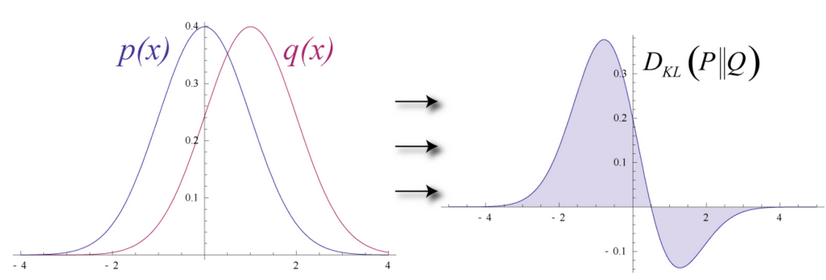
\includegraphics[width = 0.7\linewidth]{thesisfigures/KL_divergence_RBM.png}
 \caption{Illustration of the Kullback-Leibler divergence which measures the difference between two probability distributions $p(x)$ and $q(x)$.
 Figure taken from \href{https://deeplearning4j.org/restrictedboltzmannmachine}{here}.}
 \label{fig:KLdivergence}
\end{figure}



When the goal of the training is to approximate a probability distribution, as it is in generative modeling, another relevant measure is the \textbf{Kullback-Leibler divergence}, also known as the relative entropy or Shannon entropy (see figure \ref{fig:KLdivergence}). It is a non-symmetric measure of the dissimilarity between two probability density functions $p$ and $q$. If $p$ is the unkown probability which we approximate with $q$, we can measure the difference by
\begin{align}
	\text{KL}(p||q) = \int_{-\infty}^{\infty} p (\bm{x}) \log \frac{p(\bm{x})}{q(\bm{x})} \dif \bm{x}.
\end{align}
Thus, the Kullback-Leibler divergence between the distribution of the training data $f(\bm{x})$ and the model distribution $p(\bm{x}| \bm{\theta})$ is
\begin{align}
	\text{KL} (f(\bm{x})|| p(\bm{x}| \bm{\theta})) =& \int_{-\infty}^{\infty}
	f (\bm{x}) \log \frac{f(\bm{x})}{p(\bm{x}| \bm{\theta})} \dif \bm{x} \\
	=& \int_{-\infty}^{\infty} f(\bm{x}) \log f(\bm{x}) \dif \bm{x} - \int_{-\infty}^{\infty} f(\bm{x}) \log
	p(\bm{x}| \bm{\theta}) \dif \bm{x} \\
	%=& \mathbb{E}_{f(\bm{x})} (\log f(\bm{x})) - \mathbb{E}_{f(\bm{x})} (\log p(\bm{x}| \bm{\theta}))
	=& \langle \log f(\bm{x}) \rangle_{f(\bm{x})} - \langle \log p(\bm{x}| \bm{\theta}) \rangle_{f(\bm{x})} \\
	=& \langle \log f(\bm{x}) \rangle_{data} + \langle E(\bm{x}) \rangle_{data} + \log Z \\
	=& \langle \log f(\bm{x}) \rangle_{data} + \mathcal{C}_{LL} .
\end{align}
The first term is constant with respect to $\bm{\theta}$ since $f(\bm{x})$ is independent of $\bm{\theta}$. Thus the Kullback-Leibler Divergence is minimal when the second term is minimal. The second term is the log-likelihood cost function, hence minimizing the Kullback-Leibler divergence is equivalent to maximizing the log-likelihood.

To further understand generative models it is useful to study the gradient of the cost function which is needed in order to minimize it using methods presented in section \ref{sec:GD}. As in statistical physics the partition function is the generating function of expectation values, in particular there are mathematical relationships between expectation values and the log-partition function. In this case we have \cite{Mehta2018}

\begin{align}
	\langle \frac{ \partial E(\bm{x}; \theta_i) } { \partial \theta_i} \rangle_{model}
	= \int p(\bm{x}| \bm{\theta}) \frac{ \partial E(\bm{x}; \theta_i) } { \partial \theta_i} \dif \bm{x} 
	= -\frac{\partial \log Z(\theta_i)}{ \partial  \theta_i} .
\end{align}

Here $\langle \cdot \rangle_{model}$ is the expectation value over the model probability distribution $p(\bm{x}| \bm{\theta})$.
Using this relationship we can express the gradient of the cost function as
\begin{align}
	\frac{\partial \mathcal{C}_{LL}}{\partial \theta_i}
	=& \langle \frac{ \partial E(\bm{x}; \theta_i) } { \partial \theta_i} \rangle_{data} + \frac{\partial \log Z(\theta_i)}{ \partial  \theta_i} \\
	=& \langle \frac{ \partial E(\bm{x}; \theta_i) } { \partial \theta_i} \rangle_{data} - \langle \frac{ \partial E(\bm{x}; \theta_i) } { \partial \theta_i} \rangle_{model} \\
	%=& \langle O_i(\bm{x}) \rangle_{data} - \langle O_i(\bm{x}) \rangle_{model}
\end{align}
This expression shows that the gradient of the log-likelihood cost function is a \textbf{difference of moments}, with one calculated from the data and one calculated from the model. The data-dependent term is called the \textbf{positive phase} and the model-dependent term is called the \textbf{negative phase} of the gradient. We see now that minimizing the cost function results in lowering the energy of configurations $\bm{x}$ near points in the training data and increasing the energy of configurations not observed in the training data. That means we increase the model's probability of configurations similar to those in the training data.

The gradient of the cost function also demonstrates why gradients of unsupervised, generative models must be computed differently from for those of for example FNNs. While the data-dependent expectation value is easily calculated based on the samples $\bm{x}_i$ in the training data, we must sample from the model in order to generate samples from which to caclulate the model-dependent term. We sample from the model by using MCMC-based methods. We can not sample from the model directly because the partition function $Z$ is generally intractable.

As in supervised machine learning problems, the goal is also here to perform well on \textit{unseen} data, that is to have good generalization from the training data. The distribution $f(x)$ we approximate is not the \textit{true} distribution we wish to estimate, it is limited to the training data. Hence, in unsupervised training as well it is important to prevent overfitting to the training data. Thus it is common to add regularizers to the cost function in the same manner as described for the supervised methods.


\section{Gradient Descent Optimization}
\label{sec:GD}
Gradient descent is the most common method in machine learning for minimizing the cost function during the training stage. The goal is to iteratively update the parameters of the model in directions where the gradient of the cost function is large and negative. This procedure ensures that the parameters move towards a local minimum. In the simplest gradient descent scheme we start with initial parameter values  $\bm{\theta}_0$ and update according to
\begin{align}
	\mathbf{v}_t &= \eta_t \nabla_\theta \mathcal{C}(\bm{\theta}_t) \\
	\bm{\theta}_{t+1} &= \bm{\theta}_t - \mathbf{v}_t 	
\end{align}
where $\eta_t$ is a parameter which controls the step size and is called the \textbf{learning rate}.

To see the benefits and limitations to the gradient descent method we can compare it to Newton's method, which is  a \textit{second-order method}. In Newton's method the update $\bm{v}$ of the parameters is chosen in order to minimize the second-order Taylor expansion of the cost function:
\begin{align}
	\mathcal{C}(\bm{\theta} + \mathbf{v}) \approx \mathcal{C}(\bm{\theta}) + \nabla_\theta \mathcal{C}(\bm{\theta})\mathbf{v} + \frac{1}{2} \mathbf{v}^T H(\theta) \mathbf{v}
\end{align}
where $H(\theta)$ is the Hessian matrix of second derivatives. Differentiating this expression with respect to $\bm{v}$ and using that we should have $\nabla_\theta E(\bm{\theta} + \mathbf{v}_{opt}) = 0$ we find
\begin{align}
	0 = \nabla_\theta E(\bm{\theta}) + H(\theta) \mathbf{v}_{opt}
\end{align}
rewriting yields the update rules for Newton's method
\begin{align}
	\mathbf{v}_t &= H^{-1} (\theta_t) \nabla_\theta E(\theta_t) \\
	\bm{\theta}_{t+1} &= \bm{\theta}_t - \mathbf{v}_t
\end{align}
We cannot be sure that the Hessian is well conditioned so it is common to replace its inverse with a reregularized pseudo-inverse such as $[H(\theta_t)+\epsilon I ]^{-1}$, where $\epsilon$ is a small parameter. We see that Netwon's method has the same form as gradient descent, with the inverse Hessian acting as the learning rate. The benefit of this is that, while gradient descent has the same learning rate for all the parameters, in this case it is automatically adapted to each parameter individually, taking larger step in flat directions and smaller steps in steep directions. The reason is that the Hessian encodes the curvature of the surface, in the sense that its singular values are \textit{inversly proportional to the squares of the local curvatures of the surface}. However there are reasons why gradient descent is often preferred to second-order methods. It is an extremely intensive computational operation to calculate the Hessian. And even if one uses first-order methods to approximate the Hessian, known as quasi-Newton methods, one must still store and invert a matrix with $n^2$ entries, where $n$ is the number of parameters. \cite{Mehta2018}

The main consideration when choosing the gradient descent learning rate is a trade-off between accuracy and speed. While a small learning rate is guaranteed to converge to a local minimum, it may be very slow. A learning rate that is too big, on the other hand, can make the algorithm unstable, either oscillating around the minimum or even moving away from it, see fiugre \ref{fig:LearningRateMehta}. In the following sections we will look at some of the various improvements one can make to the simple gradient descent scheme.



\begin{figure}
\centering
 \includegraphics[width = 0.6\linewidth]{thesisfigures/LearningRateMehta.png}
 \caption{Taken from \href{https://deeplearning4j.org/restrictedboltzmannmachine}{here}}
 \label{fig:LearningRateMehta}
\end{figure}




\subsection{Momentum}
One of the simplest modifications to the simple gradient descent algorithm is to introduce a term called \textbf{momentum}, which functions as a memory of the direction the algorithm is moving in parameter space. The update rule becomes
\begin{align}
		\mathbf{v}_t =& \gamma \mathbf{v}_{t-1} + \eta_t \nabla_\theta E(\bm{\theta}_t) \\
		\bm{\theta}_{t+1} =& \bm{\theta}_t - \mathbf{v}_t,
\end{align}
where $0 \leq \gamma \leq 1$ is the momentum hyperparameter, and $\mathbf{v}_t$ becomes a moving average over the most recent gradients with $(1-\gamma)^{-1}$ setting the characteristic time scale for the memory. Introducing momentum is useful because it increases the step size in directions with persistent but small gradients, and prevents oscillations in directions with high curvature.



\subsection{RMS-prop}
As mentioned, one ideally wants to adapt the learning rate to the curvature of the landscape without having to calculate the computationally expensive inverse of the Hessian matrix of second derivatives. Over the last years a number of algorithms have been developed which achieve this by keeping track of the second moment of the gradient in addition to the gradient itself. Some of these methods include AdaGrad, AdaDelta, RMS-prop, and ADAM. We will discuss RMS-prop and the ADAM optimizer. Multiplication and division by vectors is to be taken as element-wise operations.

The RMS-prop algorithm keeps track of the second moment of the gradient with the term $\mathbf{s}_t = \mathbb{E}[\mathbf{g}_t^2]$. The update rule is then given by
\begin{align}
	\mathbf{g}_t =& \nabla_\theta E(\bm{\theta}) \\
	\mathbf{s}_t =& \beta \mathbf{s}_{t-1} + (1-\beta)\mathbf{g}_t^2 \\
	\bm{\theta}_{t+1} =& \bm{\theta}_t - \eta_t \frac{\mathbf{g}_t}{\sqrt{\mathbf{s}_t + \epsilon}}.
\end{align}
Here $\beta$ sets the averaging time of the second moment and typically has a value around $\beta=0.9$. $\eta_t$ is the learning rate, typically $10^{-3}$, and $\epsilon \sim 10^{-8}$ is a regularization constant in order to prevent divergencies. As desired this update rule ensures that the learning rate is reduced in directions where the magnitude of the gradient is consistently large. We can therefore use a larger learning rate which speeds up the process.

\subsection{ADAM}
\label{sec:adam}
The ADAM optimizer keeps a moving average of both the first and second moment of the gradient, that is $\mathbf{m}_t = \mathbb{E}[\mathbf{g}_t]$ and $\mathbf{s}_t = \mathbb{E}[\mathbf{g}_t^2]$ respectively.
\begin{align}
	\mathbf{g}_t &= \nabla_\theta E(\bm{\theta}) \\
	\mathbf{m}_t &= \beta_1 \mathbf{m}_{t-1} + (1-\beta_1) \mathbf{g}_t \\
	\mathbf{s}_t &= \beta_2 \mathbf{s}_{t-1} + (1-\beta_2) \mathbf{g}_t^2 \\
	\hat{\mathbf{m}}_t &= \frac{\mathbf{m}_t}{1-\beta_1^t} \\
	\hat{\mathbf{s}}_t &= \frac{\mathbf{s}_t}{1-\beta_2^t} \\
	\bm{\theta}_{t+1} &= \bm{\theta}_t - \eta_t \frac{\hat{\mathbf{m}}_t}{\sqrt{\hat{\mathbf{s}}_t} + \epsilon}
\end{align}
Here the variables denoted by hats represent a bias correction introduced because we estimate the moments of the gradient using a moving average. $\eta$ and $\epsilon$ are the same as for RMS-prop and $\beta_1$ and $\beta_2$ control the memory lifetime of the first and second moment, typically taken as 0.9 and 0.99 respectively.

Like in RMS-prop the effective step size of a parameter depends on the magnitude of its gradient squared. 
We can investigate this further by looking at how a single parameter $\theta_t$ is updated in terms of the variance $\bf{\sigma}_t^2 = \hat{\mathbf{s}}_t  - (\hat{\mathbf{m}}_t)^2$. The update can be written
\begin{align}
	\Delta \theta_{t+1} = -\eta_t \frac{\hat{m}_t}{\sqrt{\sigma_t^2 + m_t^2} + \epsilon} .
\end{align}
If we consider the limits of this expression we see that
\begin{itemize}
	\item  If $\sigma_t^2 \ll  \hat{m}_t^2$ then  $\Delta \theta_{t+1} \rightarrow -\eta_t$. If the variance is small while the gradient is big, meaning we are moving persistently in steep directions, the maximum step size is limited to $\eta_t$.
	\item If  $\sigma^2 \gg \hat{m}_t^2$ then $\Delta \theta_{t+1} \rightarrow -\eta_t \hat{m}_t/ \sigma_t$. This means that if the variance is big, so that there are great fluctuations in the gradient, the learning rate becomes proportional to the mean of the gradients in units of the standard deviation. This is good because the standard deviation is a natural and adaptive scale for determining whether the gradient is large or small.
\end{itemize}
In conclusion, the ADAM optimizer is able to configure the learning rate to not become too big in steep directions, avoiding oscillations and divergencies, as well as being adaptive when the gradient is experiencing large fluctuations. 

While RMS-prop and ADAM allow for using a bigger learning rate which speeds up computations some have observed that these methods might not generalize as well. Generalization refers to whether the trained model preforms well on unseen test data after having been trained on the training data and is an important goal in machine learning. 











\chapter{The Restricted Boltzmann Machine}
\label{sec:RBMchapter}
%Put in RMF section?: Hopfield network if nodes deterministic rather than stochastic.
%Where discuss DBNs?

The restricted Boltzmann machine (RBM) is an unsupervised, generative neural network which became known when Hinton \textit{et al} presented an efficient algorithm for training it \cite{Hinton2002} and soon after used it as a building block in deep belief networks, which were introduced in a series of seminal papers that coined the term deep learning and reawakened interest in artificial neural networks \cite{Hinton2006a} \cite{Hinton2006} \cite{Hinton2007}. The RBM has since been applied to a number of tasks including speech representation (Mohammed 2009), classification of images and documents (LaRochelle, Bengio 2008), video and motion capture data (taylor, hinton 2009) and more recently quantum many body methods (cite).

This chapter gives an introduction to the restricted Boltzmann machine. First, the general Boltzmann machine, then the RBM and the original variant with binary visible and hidden units, the binary-binary RBM. Finally we will look at the variant used in this work, the Gaussian-binary RBM, as well as the RBM training procedure.





%This chapter gives an introduction to the unsupervised artificial neural network RBMs. First BM and RBM, then the original RBM with binary nodes, first used in quantum problems for spin-lattice models. Then, the GB which allows for continuous values and position QM.


%This is called a localist encoding, since only one hidden unit is used to generate the response vector. This is analogous to the hypothetical notion of grandmother cells in the brain, that are able to recognize only one kind of object. By contrast, an RBM uses a distributed encoding, where many units are involved in generating each output. Models that used vector-valued hidden variables, such as (PCA examples) also use distributed encodings. \cite{Murphy2012}



\section{The Boltzmann Machine}
\label{sec:BM}


\begin{figure}
\centering
 \includegraphics[width = 0.5\linewidth]{thesisfigures/BMwikipedia.png}
 \caption{The the Boltzmann machine represented by an undirected, graphical model. Blue nodes are hidden units and white nodes are visible units. The Boltzmann machine is a complete graph, meaning each pair of nodes is connected by an edge. The nodes are stochastic, which makes it a probabilistic graphical model. Figure from \href{https://en.wikipedia.org/wiki/Boltzmann_machine}{here}.}
 \label{fig:BMwikipedia}
\end{figure}


%Product of experts (Hinton 1999 article). MRF is a special case of PoEs. (a PoE model with exponential experts is an MRF with input variables x and latent variables h, which is expressed by the Hammersley and Clifford theorem.) Since we multiply the individual probabilities of the experts, it is obvious that we only get a high overall probability if all experts assign high individual probabilities. The PoE can therefore be interpreted as a council that judges a presented sample as being important if the judgement is unanimous. This stays in contrast to a mixture model [5] where the individual probabilities for a presented sample are summed up. Consequently, in a mixture model an expert or mixture can possibly overrule the others and the overall probability will only be low if all mixtures assign low proba- bility.
%\cite{Melchior2012}

%An RBM is a special case of a product of experts (PoE) (Hinton 1999), which is so-called because we are multiplying together a set of “experts” (here, potential functions on each edge) and then normalizing, whereas in a mixture of experts, we take a convex combination of normalized distributions. The intuitive reason why PoE models might work better than a mixture is that each expert can enforce a constraint (if the expert has a value which is $\gg$ 1 or $\ll$ 1) or a “don’t care” condition (if the expert has value 1). By multiplying these experts together in di erent ways we can create “sharp” distributions which predict data which satisfies the specified constraints (Hinton and Teh 2001). For example, consider a distributed model of text. A given document might have the topics “government”, “mafia” and “playboy”. If we “multiply” the predictions of each topic together, the model may give very high probability to the word “Berlusconi”9 (Salakhutdinov and Hinton 2010). By contrast, adding together experts can only make the distribution broader (see Figure 14.17).
%\cite{Murphy2012}

%While an MRF is a particular case of a PoE, a BM is an MRF with a particular energy function that leads to a complete undirected graph as shown in Figure 8.
%This implies a fully connected network where the pairwise communication between two units is symmetrical. The activation of each node is given by the sum over all values of its incoming connections. 


The Boltzmann machine \cite{Ackley1985} is a type of Markov Random Field (section \ref{sec:MRF}) where each pair of nodes is connected by an edge (see figure \ref{fig:BMwikipedia}). This means it is a fully connected network, or a \textbf{complete graph}. Furthermore the nodes are defined as either \textbf{visible} nodes, denoted by $\bm{x}$, or \textbf{hidden} nodes, denoted $\bm{h}$. The visible nodes are the input and output. The hidden nodes are latent variables of which the purpose is to encode complex interactions between the visible nodes. 

%Latent or hidden variables are a powerful yet elegant way to encode sophisticated correlations between observ- able features. The underlying reason for this is that marginalizing over a subset of variables – “integrating out” degrees of freedom in the language of physics – in- duces complex interactions between the remaining vari- ables. The idea that integrating out variables can lead to complex correlations is a familiar component of many physical theories. For example, when considering free electrons living on a lattice, integrating out phonons gives rise to higher-order electron-electron interactions (e.g. su- perconducting or magnetic correlations). More generally, in the Wilsonian renormalization group paradigm, all ef- fective field theories can be thought of as arising from integrating out high-energy degrees of freedom (Wilson and Kogut, 1974).
%Generative models with latent variables run this logic in reverse – encode complex interactions between visible variables by introducing additional, hidden variables that interact with visible degrees of freedom in a simple man- ner, yet still reproduce the complex correlations between visible degrees in the data once marginalized over (in- tegrated out). This allows us to encode complex higher- order interactions between the visible variables using sim- pler interactions at the cost of introducing new latent variables/degrees of freedom. This trick is also widely exploited in physics (e.g. in the Hubbard-Stratonovich transformation (Hubbard, 1959; Stratonovich, 1957) or the introduction of ghost fields in gauge theory (Faddeev and Popov, 1967)).

The joint probability density function of the variables is, similar to the MRF in equation \ref{eq:MRFhidden}, given by

\begin{align}
	p_{BM}(\bm{x}, \bm{h}) = \frac{1}{Z_{BM}} e^{-\frac{1}{T}E_{BM}(\bm{x}, \bm{h})} ,
\end{align}
with the partition function 
\begin{align}
	Z_{BM} = \int \int e^{-\frac{1}{T} E_{BM}(\tilde{\bm{x}}, \tilde{\bm{h}})} \dif \tilde{\bm{x}} \dif \tilde{\bm{h}} .
\end{align}

$T$ is a physics-inspired parameter named temperature and will be assumed to be 1 unless otherwise stated. The energy function of the Boltzmann machine determines the interactions between the nodes and is defined  

\begin{align}
	E_{BM}(\bm{x}, \bm{h}) =& - \sum_{i, k}^{M, K} a_i^k \alpha_i^k (x_i)
	- \sum_{j, l}^{N, L} b_j^l \beta_j^l (h_j) 
	- \sum_{i,j,k,l}^{M,N,K,L} \alpha_i^k (x_i) w_{ij}^{kl} \beta_j^l (h_j) \nonumber \\
	&- \sum_{i, m=i+1, k}^{M, M, K} \alpha_i^k (x_i) v_{im}^k \alpha_m^k (x_m)
	- \sum_{j,n=j+1,l}^{N,N,L} \beta_j^l (h_j) u_{jn}^l \beta_n^l (h_n).
\end{align}
Here $\alpha_i^k (x_i)$ and $\beta_j^l (h_j)$ are one-dimensional transfer functions or mappings from the given input value to the desired feature value. They can be arbitrary functions of the input variables and are independent of the parameterization (parameters referring to weight and biases), meaning they are not affected by training of the model. The indices $k$ and $l$ indicate that there can be multiple transfer functions per variable.
Furthermore, $a_i^k$ and $b_j^l$ are the visible and hidden bias. $w_{ij}^{kl}$ are weights of the \textbf{inter-layer} connection terms which connect visible and hidden units. $ v_{im}^k$ and $u_{jn}^l$ are weights of the \textbf{intra-layer} connection terms which connect the visible units to each other and the hidden units to each other, respectively.

\begin{comment}
\begin{itemize}
	\item $\alpha_i^k (x_i), \beta_j^l (h_j) $= One dimensional transfer functions, mapping a given input value to a desired feature value. They are sufficient statistics of the model and can be arbitrary non-parametrized functions of the input variable $x_i$ or $h_j$ respectively, but they need to be independent of the parametrization.
	\item $k, l $= These indices denote there can be multiple transfer funcs pr variable.
	\item $a_i^k,  b_j^l$= appear in the first and second term which only depends ont he visible and hidden units respectively. Thus they could be interpreted as the corresponding visible and hidden bias respectively.
	\item $w_{ij}^{kl}$ = inter layer connection term, connects the visible and hidden bias, respectively.
	\item $ v_{im}^k, u_{jn}^l$ = intra layer connection terms, connecting the visible units to each other, and the hidden units to each other, respectively.
\end{itemize}
\end{comment}

%This formalism allows to define even complexer BMs where more than two units interact with each other, named higher order BMs [36]. But a major disadvantage of BMs in general is that it is usually intractable to calculate the partition function since the integration over all possible states is only computable for small toy prob- lems.
%Therefore, training BMs is usually done by approximations using sampling methods [5], which will be described in detail later. So far it is just important to note that for those sampling methods we need to be able to calculate the conditional probability of the visible units given the hidden units and vice versa. Using Bayes theorem we can derive the conditional probability of the hidden units given the visible values and vice versa.



\subsection{Restricted Boltzmann Machines}
\label{sec:RBM}

\begin{figure}
\centering
 \includegraphics[width = 0.6\linewidth]{thesisfigures/RBMmehta.png}
 \caption{The bipartite graph structure of the restricted Boltzmann machine. In contrast to the general Boltzmann machine there are no connections within layers. Figure from \cite{Mehta2018}.}
 \label{fig:RBMmehta}
\end{figure}


The RBM was originally introduced in \cite{Smolensky1986} with the name \textbf{harmonium}, since the energy function was referred to as the \textit{harmony} at the time. It was introduced as the restricted Boltzmann machine by Hinton in \cite{Hinton2002}.
The RBM is a simpler version of the Boltzmann machine where there are no connections within layers. This means the units within the visible layer are conditionally independent of each other and the same for the units in the hidden layer. This makes the RBM a \textbf{bipartite} graph, see figure \ref{fig:RBMmehta}.

%A simplification where all lateral connections between visible units and all lateral connections between hidden units are removed, is a so called Restricted Boltzmann Machine (RBM). The RBMs structure is a bipartite graph where visible and hidden units are pairwise conditionally independent, shown in Figure 9.

%The major advantage of RBMs is that the units of the visible layer are conditional independent and so are the units of the hidden layer. This 

The conditional independency within layers leads to a factorization property of RBMs when marginalizing out the visible or hidden units. The integral over all possible states of the visible layer factorizes into a product of one
dimensional integrals over all possible values for the corresponding unit. Therefore, conditional probabilities can be computed efficiently. Having the conditional probabilities means Gibbs sampling, a simpler version of Metropolis-Hastings sampling, can be employed. 

\subsubsection{Energy Function}

We remove the intra-layer connections by setting $v_{im}$ and $u_{jn}$ to zero. The expression for the energy of the RBM is then
\begin{align}
	E_{RBM}(\bm{x}, \bm{h}) = - \sum_{i, k}^{M, K} a_i^k \alpha_i^k (x_i)
	- \sum_{j, l}^{N, L} b_j^l \beta_j^l (h_j) 
	- \sum_{i,j,k,l}^{M,N,K,L} \alpha_i^k (x_i) w_{ij}^{kl} \beta_j^l (h_j). \label{eq:RBMenergy}
\end{align}

%\subsubsection{Joint Probability Density Function}

\begin{comment}
\subsubsection{Marginal Probability Density Functions}
\begin{align}
	P_{RBM} (\bm{x}) =& \int P_{RBM} (\bm{x}, \tilde{\bm{h}}) \dif \tilde{\bm{h}} \nonumber \\
	=& \frac{1}{Z_{RBM}} \int e^{-E_{RBM} (\bm{x}, \tilde{\bm{h}}) } \dif \tilde{\bm{h}} \nonumber \\
	=& \frac{1}{Z_{RBM}} \int e^{\sum_{i, k} a_i^k \alpha_i^k (x_i)
	+ \sum_{j, l} b_j^l \beta_j^l (\tilde{h}_j) 
	+ \sum_{i,j,k,l} \alpha_i^k (x_i) w_{ij}^{kl} \beta_j^l (\tilde{h}_j)} 
	\dif \tilde{\bm{h}} \nonumber \\
	=& \frac{1}{Z_{RBM}} e^{\sum_{i, k} a_i^k \alpha_i^k (x_i)}
	\int \prod_j^N e^{\sum_l b_j^l \beta_j^l (\tilde{h}_j) 
	+ \sum_{i,k,l} \alpha_i^k (x_i) w_{ij}^{kl} \beta_j^l (\tilde{h}_j)} \dif \tilde{\bm{h}} \nonumber \\
	=& \frac{1}{Z_{RBM}} e^{\sum_{i, k} a_i^k \alpha_i^k (x_i)}
	\biggl( \int e^{\sum_l b_1^l \beta_1^l (\tilde{h}_1) + \sum_{i,k,l} \alpha_i^k (x_i) w_{i1}^{kl} \beta_1^l (\tilde{h}_1)} \dif  \tilde{h}_1 \nonumber \\
	& \times \int e^{\sum_l b_2^l \beta_2^l (\tilde{h}_2) + \sum_{i,k,l} \alpha_i^k (x_i) w_{i2}^{kl} \beta_2^l (\tilde{h}_2)} \dif  \tilde{h}_2 \nonumber \\
	& \times ... \nonumber \\
	& \times \int e^{\sum_l b_N^l \beta_N^l (\tilde{h}_N) + \sum_{i,k,l} \alpha_i^k (x_i) w_{iN}^{kl} \beta_N^l (\tilde{h}_N)} \dif  \tilde{h}_N \biggr) \nonumber \\
	=& \frac{1}{Z_{RBM}} e^{\sum_{i, k} a_i^k \alpha_i^k (x_i)}
	\prod_j^N \int e^{\sum_l b_j^l \beta_j^l (\tilde{h}_j) + \sum_{i,k,l} \alpha_i^k (x_i) w_{ij}^{kl} \beta_j^l (\tilde{h}_j)}  \dif \tilde{h}_j
\end{align}

Similarly
\begin{align}
	P_{RBM} (\bm{h}) =& \frac{1}{Z_{RBM}} \int e^{-E_{RBM} (\tilde{\bm{x}}, \bm{h})} \dif \tilde{\bm{x}} \nonumber \\
	=& \frac{1}{Z_{RBM}} e^{\sum_{j, l} b_j^l \beta_j^l (h_j)}
	\prod_i^M \int e^{\sum_k a_i^k \alpha_i^k (\tilde{x}_i)
	+ \sum_{j,k,l} \alpha_i^k (\tilde{x}_i) w_{ij}^{kl} \beta_j^l (h_j)} \dif \tilde{x}_i
\end{align}

\subsubsection{Conditional Probability Density Functions}
Using Bayes theorem:
\begin{align}
	P_{RBM} (\bm{h}|\bm{x}) =& \frac{P_{RBM} (\bm{x}, \bm{h})}{P_{RBM} (\bm{x})} \nonumber \\
	=& \frac{\frac{1}{Z_{RBM}} e^{\sum_{i, k} a_i^k \alpha_i^k (x_i)
	+ \sum_{j, l} b_j^l \beta_j^l (h_j) 
	+ \sum_{i,j,k,l} \alpha_i^k (x_i) w_{ij}^{kl} \beta_j^l (h_j)}}
	{\frac{1}{Z_{RBM}} e^{\sum_{i, k} a_i^k \alpha_i^k (x_i)}
	\prod_j^N \int e^{\sum_l b_j^l \beta_j^l (\tilde{h}_j) + \sum_{i,k,l} \alpha_i^k (x_i) w_{ij}^{kl} \beta_j^l (\tilde{h}_j)}  \dif \tilde{h}_j} \nonumber \\
	=& \prod_j^N \frac{e^{\sum_l b_j^l \beta_j^l (h_j) + \sum_{i,k,l} \alpha_i^k (x_i) w_{ij}^{kl} \beta_j^l (h_j)} }
	{\int e^{\sum_l b_j^l \beta_j^l (\tilde{h}_j) + \sum_{i,k,l} \alpha_i^k (x_i) w_{ij}^{kl} \beta_j^l (\tilde{h}_j)}  \dif \tilde{h}_j}
\end{align}
Similarly
\begin{align}
	P_{RBM} (\bm{x}|\bm{h}) =&  \frac{P_{RBM} (\bm{x}, \bm{h})}{P_{RBM} (\bm{h})} \nonumber \\
	=& \prod_i^M \frac{e^{\sum_k a_i^k \alpha_i^k (x_i)
	+ \sum_{j,k,l} \alpha_i^k (x_i) w_{ij}^{kl} \beta_j^l (h_j)}}
	{\int e^{\sum_k a_i^k \alpha_i^k (\tilde{x}_i)
	+ \sum_{j,k,l} \alpha_i^k (\tilde{x}_i) w_{ij}^{kl} \beta_j^l (h_j)} \dif \tilde{x}_i}
\end{align}
\end{comment}


\subsection{Binary-Binary Restricted Boltzmann Machines}
The original RBM had binary visible and hidden nodes. They were showned to be universal approximators of discrete distributions in \cite{LeRoux2008}. It was also shown that adding hidden units yields strictly improved modelling power. The common choice of binary values are 0 and 1. However, in some physics applications, -1 and 1 might be a more natural choice. We will here use 0 and 1.


\subsubsection{Energy Function}

\begin{table*}\centering
\ra{1.3}
\caption{This table shows how the terms in the restricted Boltzmann machine (RBM) energy function (equation \ref{eq:RBMenergy}) should be implemented in order to yield the binary-binary restricted boltzmann machine, that is an RBM where both visible and hidden units take binary values. }
\label{tab:BBrbm}
\begin{tabular}{lll}
\toprule
\toprule
Transfer functions & Biases & Weights \\ 
\midrule 
$\alpha_i^1 (x_i) = x_i$ & $a_i^1 = a_i$  & $w_{ij}^{11} = w_{ij}$ \\
$\beta_j^1 (h_j) = h_j$  & $b_j^1 = b_j$  &  \\
\bottomrule
\bottomrule
\end{tabular}
\end{table*}

Table \ref{tab:BBrbm} shows how the RBM energy function should be implemented for the binary-binary RBM, using only one transfer function, the identity, for each layer. This results in the energy

\begin{align}
	E_{BB}(\bm{x}, \mathbf{h}) = - \sum_i^M x_i a_i- \sum_j^N b_j h_j - \sum_{i,j}^{M,N} x_i w_{ij} h_j.
	\label{eq:BBenergy}
\end{align}


\subsubsection{Joint Probability Density Function}
With the energy given in equation \ref{eq:BBenergy}, the joint probability density function of the units in the binary-binary RBM becomes
\begin{align}
	p_{BB}(\bm{x}, \bm{h}) =& \frac{1}{Z_{BB}} e^{\sum_i^M a_i x_i + \sum_j^N b_j h_j + \sum_{ij}^{M,N} x_i w_{ij} h_j} \\
	=& \frac{1}{Z_{BB}} e^{\bm{x}^T \bm{a} + \bm{b}^T \bm{h} + \bm{x}^T \bm{W} \bm{h}}
\end{align}
with the partition function
\begin{align}
	Z_{BB} = \sum_{\bm{x}, \bm{h}} e^{\bm{x}^T \bm{a} + \bm{b}^T \bm{h} + \bm{x}^T \bm{W} \bm{h}} .
\end{align}

\subsubsection{Marginal Probability Density Functions}
In order to find the probability of any configuration of the visible units we derive the marginal probability density function.

\begin{align}
	p_{BB} (\bm{x}) =& \sum_{\bm{h}} p_{BB} (\bm{x}, \bm{h}) \\
	=& \frac{1}{Z_{BB}} \sum_{\bm{h}} e^{\bm{x}^T \bm{a} + \bm{b}^T \bm{h} + \bm{x}^T \bm{W} \bm{h}} \nonumber \\
	=& \frac{1}{Z_{BB}} e^{\bm{x}^T \bm{a}} \sum_{\bm{h}} e^{\sum_j^N (b_j + \bm{x}^T \bm{w}_{\ast j})h_j} \nonumber \\
	=& \frac{1}{Z_{BB}} e^{\bm{x}^T \bm{a}} \sum_{\bm{h}} \prod_j^N e^{ (b_j + \bm{x}^T \bm{w}_{\ast j})h_j} \nonumber \\
	=& \frac{1}{Z_{BB}} e^{\bm{x}^T \bm{a}} \bigg ( \sum_{h_1} e^{(b_1 + \bm{x}^T \bm{w}_{\ast 1})h_1}
	\times \sum_{h_2} e^{(b_2 + \bm{x}^T \bm{w}_{\ast 2})h_2} \times \nonumber \\
	& ... \times \sum_{h_2} e^{(b_N + \bm{x}^T \bm{w}_{\ast N})h_N} \bigg ) \nonumber \\
	=& \frac{1}{Z_{BB}} e^{\bm{x}^T \bm{a}} \prod_j^N \sum_{h_j} e^{(b_j + \bm{x}^T \bm{w}_{\ast j}) h_j} \nonumber \\
	=& \frac{1}{Z_{BB}} e^{\bm{x}^T \bm{a}} \prod_j^N (1 + e^{b_j + \bm{x}^T \bm{w}_{\ast j}}) .
\end{align}

A similar derivation yields the marginal probability of the hidden units

\begin{align}
	p_{BB} (\bm{h}) = \frac{1}{Z_{BB}} e^{\bm{b}^T \bm{h}} \prod_i^M (1 + e^{a_i + \bm{w}_{i\ast}^T \bm{h}}) .
\end{align}


\subsubsection{Conditional Probability Density Functions}
We derive the probability of the hidden units given the visible units using Bayes' rule:
\begin{align}
	p_{BB} (\bm{h}|\bm{x}) =& \frac{p_{BB} (\bm{x}, \bm{h})}{p_{BB} (\bm{x})} \nonumber \\
	=& \frac{ \frac{1}{Z_{BB}}  e^{\bm{x}^T \bm{a} + \bm{b}^T \bm{h} + \bm{x}^T \bm{W} \bm{h}} }
	        {\frac{1}{Z_{BB}} e^{\bm{x}^T \bm{a}} \prod_j^N (1 + e^{b_j + \bm{x}^T \bm{w}_{\ast j}})} \nonumber \\
	=& \frac{  e^{\bm{x}^T \bm{a}} e^{ \sum_j^N (b_j + \bm{x}^T \bm{w}_{\ast j} ) h_j} }
	        { e^{\bm{x}^T \bm{a}} \prod_j^N (1 + e^{b_j + \bm{x}^T \bm{w}_{\ast j}})} \nonumber \\
	=& \prod_j^N \frac{ e^{(b_j + \bm{x}^T \bm{w}_{\ast j} ) h_j}  }
	{1 + e^{b_j + \bm{x}^T \bm{w}_{\ast j}}} \nonumber \\
	=& \prod_j^N p_{BB} (h_j| \bm{x}) .
\end{align}
From this we find the probability of a hidden unit being "on" or "off":
\begin{align}
	p_{BB} (h_j=1 | \bm{x}) =&   \frac{ e^{(b_j + \bm{x}^T \bm{w}_{\ast j} ) h_j}  }
	{1 + e^{b_j + \bm{x}^T \bm{w}_{\ast j}}} \\
	=&  \frac{ e^{(b_j + \bm{x}^T \bm{w}_{\ast j} )}  }
	{1 + e^{b_j + \bm{x}^T \bm{w}_{\ast j}}} \\
	=&  \frac{ 1 }{1 + e^{-(b_j + \bm{x}^T \bm{w}_{\ast j})} } ,
\end{align}
and
\begin{align}
	p_{BB} (h_j=0 | \bm{x}) =\frac{ 1 }{1 + e^{b_j + \bm{x}^T \bm{w}_{\ast j}} } .
\end{align}

We see that the outcome is the sigmoid function, the same as is frequently used as non-linear activation functions in feedforward neural networks (figure \ref{fig:FNNactivationsMehta}).

%From Equation 27.101, we see that we activate hidden node k in proportion to how much the input vector v “looks like” the weight vector w:,k (up to scaling factors). Thus each hidden node captures certain features of the input, as encoded in its weight vector, similar to a feedforward neural network. \cite{Murphy}

Similarly we have that the conditional probability of the visible units given the hidden are
\begin{align}
	p_{BB} (\bm{x}|\bm{h}) =& \prod_i^M \frac{ e^{ (a_i + \bm{w}_{i\ast}^T \bm{h}) x_i} }{ 1 + e^{a_i + \bm{w}_{i\ast}^T \bm{h}} } \\
	&= \prod_i^M p_{BB} (x_i | \bm{h}) .
\end{align}
Thus
\begin{align}
	p_{BB} (x_i=1 | \bm{h}) =& \frac{1}{1 + e^{-(a_i + \bm{w}_{i\ast}^T \bm{h} )}} \\
	p_{BB} (x_i=0 | \bm{h}) =& \frac{1}{1 + e^{a_i + \bm{w}_{i\ast}^T \bm{h} }} .
\end{align}






\subsection{Gaussian-Binary Restricted Boltzmann Machines}
%Other types of units: In the original definition of BMs [2], the visible and hidden units have binary values. However, in most cases the input data is coming from a continuous rather than a binary domain. Therefore, it would be of most interest to have the opportunity to choose continuous units as well. An easy way, making the original BM handle continuous data is simply to rescale the data into the interval [0, 1] and considering it as the probability for the corresponding unit taking the value one. However, the model is still assuming an underlying binary representation, so that this variant usually works not very well. If we assume the data coming truly from the interval $[0, \infty)$ the conditional prob- abilities (97) become exponential densities. This causes the normalization constant not to exist in each case so that truncated exponentials over the interval [0,1] are used instead, which leads to the so called Truncated Exponential RBMs [15] A natural assumption when dealing with continuous variables is assuming them to be Gaussian distributed and therefore, a distribution over R . This leads to the so called Gaussian-Binary RBM, which has been used successfully to model continuous domains and will be discussed in the next chapter. So far we considered only the visible layer to have continuous values but one can also think of RBMs with continuous visible and hidden layer like a Gaussian-Gaussian RBM for example. But as we will see, training an RBM with continuous visible and binary hidden layer tends to be difficult already. Furthermore this training issue be- comes crucial when having only continuous units since they get much more effected to sampling noise. This makes them uninteresting in practice although a completely continuous network seems to be the more powerful configuration. \cite{Melchior2012}

% Also discussion in Learning a Generative Model of Images by Factoring Appearance and Shape
In a number of problems the values we want to model are not binary, but continuous. There are several ways one might accomodate this. One way is the Gaussian-binary RBM \cite{Welling2005}. In this model the hidden units are still binary, while the visible units are assumed to take real values $x_i \in [-\infty, \infty]$ and be normally distributed with variance $\sigma_i^2$. 

\subsubsection{Energy Function}



\begin{table*}\centering
\ra{1.3}
\caption{This table shows how the terms in the restricted Boltzmann machine (RBM) energy function (equation \ref{eq:RBMenergy}) should be implemented in order to yield the Gaussian-binary restricted boltzmann machine, that is an RBM where the visible units take continuous values and the hidden units take binary values.}
\label{tab:GBrbm}
\begin{tabular}{lll}
\toprule
\toprule
Transfer functions & Biases & Weights \\ 
\midrule 
$\alpha_i^1 (x_i) = -x_i^2$  & $a_i^1 = \frac{1}{2\sigma_i^2}$      & $w_{ij}^{11} = 0$ \\
$\alpha_i^2 (x_i) = x_i$     & $a_i^2 = \frac{a_i}{\sigma_i^2}$     & $w_{ij}^{21} = \frac{w_{ij}}{\sigma_i^2}$ \\
$\alpha_i^3 (x_i) = 1$       & $a_i^3 = -\frac{a_i^2}{2\sigma_i^2}$ & $w_{ij}^{31} = 0$ \\
$\beta_j^1 (h_j) = h_j$      & $b_j^1 = b_j$                        &  \\
\bottomrule
\bottomrule
\end{tabular}
\end{table*}

We find the energy function of the Gaussian-binary RBM by implementing the RBM energy as shown in table \ref{tab:GBrbm}. As seen there are now three transfer functions for the visible units ($K=3$) and one for the hidden units ($L=1$).
Inserting into the expression for $E_{RBM}(\bm{x},\bm{h})$ in equation \ref{eq:RBMenergy} results in the energy
\begin{align}
	E_{GB}(\bm{x}, \bm{h}) =& \sum_i^M \frac{(x_i - a_i)^2}{2\sigma_i^2}
	- \sum_j^N b_j h_j 
	-\sum_{ij}^{M,N} \frac{x_i w_{ij} h_j}{\sigma_i^2} \nonumber \\
	=& \norm*{\frac{\bm{x} -\bm{a}}{2\bm{\sigma}}}^2 - \bm{b}^T \bm{h} 
	- (\frac{\bm{x}}{\bm{\sigma}^2})^T \bm{W}\bm{h} . \label{eq:GBenergy}
\end{align}

%adress sigma squared or not.

\subsubsection{Joint Probability Density Function}
Given the energy in equation \ref{eq:GBenergy}, joint probability density function of the Gaussian-binary RBM is
\begin{align}
	p_{GB} (\bm{x}, \bm{h}) =& \frac{1}{Z_{GB}} e^{-\norm*{\frac{\bm{x} -\bm{a}}{2\bm{\sigma}}}^2 + \bm{b}^T \bm{h} 
	+ (\frac{\bm{x}}{\bm{\sigma}^2})^T \bm{W}\bm{h}} \nonumber \\
	=& \frac{1}{Z_{GB}} e^{- \sum_i^M \frac{(x_i - a_i)^2}{2\sigma_i^2}
	+ \sum_j^N b_j h_j 
	+\sum_{ij}^{M,N} \frac{x_i w_{ij} h_j}{\sigma_i^2}} \nonumber \\
	=& \frac{1}{Z_{GB}} \prod_{ij}^{M,N} e^{-\frac{(x_i - a_i)^2}{2\sigma_i^2}
	+ b_j h_j 
	+\frac{x_i w_{ij} h_j}{\sigma_i^2}} ,
\end{align}
%=& \frac{1}{Z_{GB}} \prod_{ij}^{M,N} \phi_{GB_{ij}} (x_i, h_j) ,

with the partition function given by
\begin{align}
	Z_{GB} =& \int \sum_{\tilde{\bm{h}}}^{\tilde{\bm{H}}} e^{-\norm*{\frac{\tilde{\bm{x}} -\bm{a}}{2\bm{\sigma}}}^2 + \bm{b}^T \tilde{\bm{h}} 
	+ (\frac{\tilde{\bm{x}}}{\bm{\sigma}^2})^T \bm{W}\tilde{\bm{h}}} \dif \tilde{\bm{x}} .
\end{align}
%=& \int \sum_{\tilde{\bm{h}}}^{\tilde{\bm{H}}} \prod_{ij}^{M, N} \phi_{GB_{ij}} (\tilde{x}_i, \tilde{h}_j) \dif \tilde{\bm{x}} .

\subsubsection{Marginal Probability Density Functions}
We proceed to find the marginal probability densitites of the Gaussian-binary RBM. We first marginalize over the binary hidden units to find $p_{GB} (\bm{x})$

\begin{align}
	p_{GB} (\bm{x}) =& \sum_{\tilde{\bm{h}}}^{\tilde{\bm{H}}} p_{GB} (\bm{x}, \tilde{\bm{h}}) \nonumber \\
	=& \frac{1}{Z_{GB}} \sum_{\tilde{\bm{h}}}^{\tilde{\bm{H}}} 
	e^{-\norm*{\frac{\bm{x} -\bm{a}}{2\bm{\sigma}}}^2 + \bm{b}^T \tilde{\bm{h}} 
	+ (\frac{\bm{x}}{\bm{\sigma}^2})^T \bm{W}\tilde{\bm{h}}} \nonumber \\
	=& \frac{1}{Z_{GB}} e^{-\norm*{\frac{\bm{x} -\bm{a}}{2\bm{\sigma}}}^2}
	\prod_j^N (1 + e^{b_j + (\frac{\bm{x}}{\bm{\sigma}^2})^T \bm{w}_{\ast j}} ) .
\end{align}

We next marginalize over the visible units. This is the first time we marginalize over continuous values. We rewrite the exponential factor dependent on $\bm{x}$ as a Gaussian function before we integrate in the last step.

\begin{align}
	p_{GB} (\bm{h}) =& \int p_{GB} (\tilde{\bm{x}}, \bm{h}) \dif \tilde{\bm{x}} \nonumber \\
	=& \frac{1}{Z_{GB}} \int e^{-\norm*{\frac{\tilde{\bm{x}} -\bm{a}}{2\bm{\sigma}}}^2 + \bm{b}^T \bm{h} 
	+ (\frac{\tilde{\bm{x}}}{\bm{\sigma}^2})^T \bm{W}\bm{h}} \dif \tilde{\bm{x}} \nonumber \\
	=& \frac{1}{Z_{GB}} e^{\bm{b}^T \bm{h} } \int \prod_i^M
	e^{- \frac{(\tilde{x}_i - a_i)^2}{2\sigma_i^2} + \frac{\tilde{x}_i \bm{w}_{i\ast}^T \bm{h}}{\sigma_i^2} } \dif \tilde{\bm{x}} \nonumber \\
	=& \frac{1}{Z_{GB}} e^{\bm{b}^T \bm{h} }
	\biggl( \int e^{- \frac{(\tilde{x}_1 - a_1)^2}{2\sigma_1^2} + \frac{\tilde{x}_1 \bm{w}_{1\ast}^T \bm{h}}{\sigma_1^2} } \dif \tilde{x}_1 \nonumber \\
	& \times \int e^{- \frac{(\tilde{x}_2 - a_2)^2}{2\sigma_2^2} + \frac{\tilde{x}_2 \bm{w}_{2\ast}^T \bm{h}}{\sigma_2^2} } \dif \tilde{x}_2 \nonumber \\
	& \times ... \nonumber \\
	&\times \int e^{- \frac{(\tilde{x}_M - a_M)^2}{2\sigma_M^2} + \frac{\tilde{x}_M \bm{w}_{M\ast}^T \bm{h}}{\sigma_M^2} } \dif \tilde{x}_M \biggr) \nonumber \\
	=& \frac{1}{Z_{GB}} e^{\bm{b}^T \bm{h}} \prod_i^M
	\int e^{- \frac{(\tilde{x}_i - a_i)^2 - 2\tilde{x}_i \bm{w}_{i\ast}^T \bm{h}}{2\sigma_i^2} } \dif \tilde{x}_i \nonumber \\
	=& \frac{1}{Z_{GB}} e^{\bm{b}^T \bm{h}} \prod_i^M
	\int e^{- \frac{\tilde{x}_i^2 - 2\tilde{x}_i(a_i + \tilde{x}_i \bm{w}_{i\ast}^T \bm{h}) + a_i^2}{2\sigma_i^2} } \dif \tilde{x}_i \nonumber \\
	=& \frac{1}{Z_{GB}} e^{\bm{b}^T \bm{h}} \prod_i^M
	\int e^{- \frac{\tilde{x}_i^2 - 2\tilde{x}_i(a_i + \bm{w}_{i\ast}^T \bm{h}) + (a_i + \bm{w}_{i\ast}^T \bm{h})^2 - (a_i + \bm{w}_{i\ast}^T \bm{h})^2 + a_i^2}{2\sigma_i^2} } \dif \tilde{x}_i \nonumber \\
	=& \frac{1}{Z_{GB}} e^{\bm{b}^T \bm{h}} \prod_i^M
	\int e^{- \frac{(\tilde{x}_i - (a_i + \bm{w}_{i\ast}^T \bm{h}))^2 - a_i^2 -2a_i \bm{w}_{i\ast}^T \bm{h} - (\bm{w}_{i\ast}^T \bm{h})^2 + a_i^2}{2\sigma_i^2} } \dif \tilde{x}_i \nonumber \\
	=& \frac{1}{Z_{GB}} e^{\bm{b}^T \bm{h}} \prod_i^M
	e^{\frac{2a_i \bm{w}_{i\ast}^T \bm{h} +(\bm{w}_{i\ast}^T \bm{h})^2 }{2\sigma_i^2}}
	\int e^{- \frac{(\tilde{x}_i - a_i - \bm{w}_{i\ast}^T \bm{h})^2}{2\sigma_i^2}}
	\dif \tilde{x}_i \nonumber \\
	=& \frac{1}{Z_{GB}} e^{\bm{b}^T \bm{h}} \prod_i^M
	\sqrt{2\pi \sigma_i^2}
	e^{\frac{2a_i \bm{w}_{i\ast}^T \bm{h} +(\bm{w}_{i\ast}^T \bm{h})^2 }{2\sigma_i^2}} .
\end{align}
%Used the physics latent variable transformation trick.
%Thus we can calculate the partition function, using factorization..?

\subsubsection{Conditional Probability Density Functions}
We finish by deriving the conditional probabilities. 
\begin{align}
	p_{GB} (\bm{h}| \bm{x}) =& \frac{p_{GB} (\bm{x}, \bm{h})}{p_{GB} (\bm{x})} \nonumber \\
	=& \frac{\frac{1}{Z_{GB}} e^{-\norm*{\frac{\bm{x} -\bm{a}}{2\bm{\sigma}}}^2 + \bm{b}^T \bm{h} 
	+ (\frac{\bm{x}}{\bm{\sigma}^2})^T \bm{W}\bm{h}}}
	{\frac{1}{Z_{GB}} e^{-\norm*{\frac{\bm{x} -\bm{a}}{2\bm{\sigma}}}^2}
	\prod_j^N (1 + e^{b_j + (\frac{\bm{x}}{\bm{\sigma}^2})^T \bm{w}_{\ast j}} ) }
	\nonumber \\
	=& \prod_j^N \frac{e^{(b_j + (\frac{\bm{x}}{\bm{\sigma}^2})^T \bm{w}_{\ast j})h_j } }
	{1 + e^{b_j + (\frac{\bm{x}}{\bm{\sigma}^2})^T \bm{w}_{\ast j}}} \nonumber \\
	=& \prod_j^N p_{GB} (h_j|\bm{x})
\end{align}

The conditional probability of a binary hidden unit $h_j$ being on or off again take the form of sigmoid functions
\begin{align}
	p_{GB} (h_j =1 | \bm{x}) =& \frac{e^{b_j + (\frac{\bm{x}}{\bm{\sigma}^2})^T \bm{w}_{\ast j} } }
	{1 + e^{b_j + (\frac{\bm{x}}{\bm{\sigma}^2})^T \bm{w}_{\ast j}}} \nonumber \\
	=& \frac{1}{1 + e^{-b_j - (\frac{\bm{x}}{\bm{\sigma}^2})^T \bm{w}_{\ast j}}} \\
	p_{GB} (h_j =0 | \bm{x}) =&
	\frac{1}{1 + e^{b_j +(\frac{\bm{x}}{\bm{\sigma}^2})^T \bm{w}_{\ast j}}} .
\end{align}

The conditional probability of the continuous $\bm{x}$ now has another form, however.
\begin{align}
	p_{GB} (\bm{x}|\bm{h})
	=& \frac{p_{GB} (\bm{x}, \bm{h})}{p_{GB} (\bm{h})} \nonumber \\
	=& \frac{\frac{1}{Z_{GB}} e^{-\norm*{\frac{\bm{x} -\bm{a}}{2\bm{\sigma}}}^2 + \bm{b}^T \bm{h} 
	+ (\frac{\bm{x}}{\bm{\sigma}^2})^T \bm{W}\bm{h}}}
	{\frac{1}{Z_{GB}} e^{\bm{b}^T \bm{h}} \prod_i^M
	\sqrt{2\pi \sigma_i^2}
	e^{\frac{2a_i \bm{w}_{i\ast}^T \bm{h} +(\bm{w}_{i\ast}^T \bm{h})^2 }{2\sigma_i^2}}}
	\nonumber \\
	=& \prod_i^M \frac{1}{\sqrt{2\pi \sigma_i^2}}
	\frac{e^{- \frac{(x_i - a_i)^2}{2\sigma_i^2} + \frac{x_i \bm{w}_{i\ast}^T \bm{h}}{2\sigma_i^2} }}
	{e^{\frac{2a_i \bm{w}_{i\ast}^T \bm{h} +(\bm{w}_{i\ast}^T \bm{h})^2 }{2\sigma_i^2}}}
	\nonumber \\
	=& \prod_i^M \frac{1}{\sqrt{2\pi \sigma_i^2}}
	\frac{e^{-\frac{x_i^2 - 2a_i x_i + a_i^2 - 2x_i \bm{w}_{i\ast}^T\bm{h} }{2\sigma_i^2} } }
	{e^{\frac{2a_i \bm{w}_{i\ast}^T \bm{h} +(\bm{w}_{i\ast}^T \bm{h})^2 }{2\sigma_i^2}}}
	\nonumber \\
	=& \prod_i^M \frac{1}{\sqrt{2\pi \sigma_i^2}}
	e^{- \frac{x_i^2 - 2a_i x_i + a_i^2 - 2x_i \bm{w}_{i\ast}^T\bm{h}
	+ 2a_i \bm{w}_{i\ast}^T \bm{h} +(\bm{w}_{i\ast}^T \bm{h})^2}
	{2\sigma_i^2} }
	\nonumber \\
	=& \prod_i^M \frac{1}{\sqrt{2\pi \sigma_i^2}}
	e^{ - \frac{(x_i - b_i - \bm{w}_{i\ast}^T \bm{h})^2}{2\sigma_i^2}} \nonumber \\
	=& \prod_i^M \mathcal{N}
	(x_i | b_i + \bm{w}_{i\ast}^T \bm{h}, \sigma_i^2) \\
	\Rightarrow p_{GB} (x_i|\bm{h}) =& \mathcal{N}
	(x_i | b_i + \bm{w}_{i\ast}^T \bm{h}, \sigma_i^2) .
\end{align}

The form of these conditional probabilities explain the name "Gaussian" and the form of the Gaussian-binary energy function. We see that the conditional probability of $x_i$ given $\bm{h}$ is a normal distribution with mean $b_i + \bm{w}_{i\ast}^T \bm{h}$ and variance $\sigma_i^2$.

\begin{comment}
\subsubsection{Further analysis of the GB-RBM - the marginal prob as a MoG}

\subsection{Gaussian-something continuous RBM?}
If we use Gaussian latent variables and Gaussian visible variables, we get an undirected version of factor analysis. However, it turns out that it is identical to the standard directed version (Marks and Movellan 2001).
If we use Gaussian latent variables and categorical observed variables, we get an undirected version of categorical PCA (Section 27.2.2). In (Salakhutdinov et al. 2007), this was applied to the Netflix collaborative filtering problem, but was found to be significantly inferior to using binary latent variables, which have more expressive power. \cite{Murphy2012}
\end{comment}




\section{Training the RBM}

The cost function of the RBM is most commonly chosen to be the negative log-likelihood and will have a similar form as discussed in \ref{sec:UnsupervisedCostfunction}. It is usually minimized using gradient descent algorithms like those discussed in \ref{sec:GD}. The one thing we will explain here however is the Gibbs sampling used to compute the gradient of the log likelihood cost function. In order to compute the gradient we need to sample configurations $\bm{x}$ from the model. This is done using MCMC methods. Since we usually know the conditional probabilities we can use a special case of Metropolis-Hastings called Gibbs sampling.

\subsection{Gibbs Sampling}
The Gibbs sampling method use the same framework as the Metropolis-Hastings algorithm (section \ref{sec:MetroHastings}) employing Markov Chains and Monte Carlo sampling. The only difference lies in how the update step is implemented. 
Recall that the Metropolis Hastings acceptance step is
\begin{align}
	A(\bm{x}^f, \bm{x}^b) = min \Big(1,  \frac{  P(\bm{x}^f) Q(\bm{x}^b| \bm{x}^f) }
	{  P(\bm{x}^b) Q(\bm{x}^f| \bm{x}^b)  }  \Big)
\end{align}

where the before and final states are denoted by $b$ and $f$ respectively and these are made superscripts in order to easily index the vector components with subscripts.

Gibbs sampling offer a smart way of choosing the proposal distribution depending on the desired distribution. Given the desired distribution $p(\bm{x}) = p(x_1, ...x_D)$ we need to formulate the proposal distribution as the conditional probability of a variable $x_i$ given all the other variables $\bm{x}_{\setminus i} = \{ x_1, ..., x_D \} \setminus \{x_i\}$.
The proposal distribution is then given by $p(x_i | \bm{x}_{\setminus i})$ and we can use it to express the desired distribution by $p(\bm{x}) = p(x_i | \bm{x}_{\setminus i}) p(\bm{x}_{\setminus i})$ . We then insert this into the Metropolis-Hastings acceptance probability. 

\begin{align}
	A(\bm{x}^f, \bm{x}^b) =& min \Big(1,  \frac{  P(\bm{x}^f) Q(\bm{x}^b| \bm{x}^f) }
	{  P(\bm{x}^b) Q(\bm{x}^f| \bm{x}^b)  }  \Big) \\
	=& min \Big(1,  \frac{  P(\bm{x}^f) P(x_i^b| \bm{x}_{\setminus i}^f) }
	{  P(\bm{x}^b) P(x_i^f| \bm{x}_{\setminus i}^b)  }  \Big) \\
	=& min \Big(1,  \frac{ P(x_i^f| \bm{x}_{\setminus i}^f)  P(\bm{x}_{\setminus i}^f) P(x_i^b| \bm{x}_{\setminus i}^f) }
	{   P(x_i^b| \bm{x}_{\setminus i}^b) P(\bm{x}_{\setminus i}^b) P(x_i^f| \bm{x}_{\setminus i}^b)  }  \Big) \\
	=& min \Big(1,  \frac{ P(x_i^f| \bm{x}_{\setminus i}^b)  P(\bm{x}_{\setminus i}^b) P(x_i^b| \bm{x}_{\setminus i}^b) }
	{   P(x_i^b| \bm{x}_{\setminus i}^b) P(\bm{x}_{\setminus i}^b) P(x_i^f| \bm{x}_{\setminus i}^b)  }  \Big) \\ \label{eq:GibbsAlgebra}
	=& 1,
\end{align}
where in \ref{eq:GibbsAlgebra} we used that only $\bm{x}_i^b$ is updated to $\bm{x}_i^f$ and so $\bm{x}_{\setminus i}^f = \bm{x}_{\setminus i}^b$. It turns out that the ratio becomes one, which means all samples are accepted in Gibbs sampling.

In the RBM the visible units are conditionally independent of each other and it is the same for the hidden units. The proposal distribution is therefore
\begin{align}
	Q(x_i | \bm{x}_{\setminus i}^b, \bm{h}) =& p_{RBM} (x_i |\bm{h}) \\
	Q(h_j | \bm{x}, \bm{h}_{\setminus j}^b) =& p_{RBM} (h_j |\bm{x}). 
\end{align}



\begin{comment}
\subsection{Notes from publications (not section in the final thesis)}

\begin{itemize}
	\item \textbf{Summary from}
	\begin{itemize}
		\item \textbf{2017: Wang, Melchior, Wiskott: Gaussian-binary Restricted Boltzmann Machines on Modeling Natural Image Statistics} \cite{Melchior2017}
\end{itemize}
	\item First proposed by
	\begin{itemize}
		\item 2005 Welling, Rosen-Zvi, Hinton: Exponential Family Harmoniums with an Application to Information Retrieval \cite{Welling2005}
	\end{itemize}
	\item A common choice når man trenger cont visibles, ref
	\begin{itemize}
		\item 2009 A. Krizhevsky: Learning multiple layers of features from tiny images (master's thesis) \cite{Krizhevsky2009}
		\item 2011 Cho, Ilin, Raiko: Improved learning of gaussian-bernoulli restricted boltzmann machines \cite{Cho2011}
	\end{itemize}
	\item Training known to be hard, modifiactions to improve it proposed by:
	\begin{itemize}
		\item 2007 Lee, Ekanadham, Ng: Used a sparse penalty during training, allowing them to learn meaningful features from natural image patches (Sparse deep belief net model for visual area v2) \cite{Lee2008}
		\item 2009 A. Krizhevsky: Trained GRBMs on natural images and concluded the difficulties are mainly due to the existence of high-frequency noise in the images, which further prevents the model from learning the important structures. (referenced above) \cite{Krizhevsky2009}
		\item 2011 Theis, Gerwinn, Sinz, Bethge: Illustrates that in terms of likelihood estimation GRBMs are already outperformed by simple mixture models. (In all likelihood, deep belief is not enough) \cite{Theis2011}
		\item Focus on improving the model in the view of generative models
		\begin{itemize}
			\item 2010 Ranzato, Krizhevsky, Hinton: Factored 3-way restricted boltzmann machines for modeling natural images \cite{Ranzato2010}
			\item 2010 Ranzato, Hinton: Modeling pixel means and covariances using factorized third-order boltzmann machines \cite{Ranzato2010a}
			\item 2011 Courville, Bergstra, Bengio: A spike and slab restricted boltzmann machine \cite{Courville2011}
			\item 2011 Le Roux, Heess, Shotton, Winn: Learning a generative model of images by factoring appearance and shape \cite{LeRoux2011}
		\end{itemize}
		\item 2011 Cho, Ilin, Raiko: Suggested the failure of GRBMs is due to the training algo and proposed some modifications to overcome the difficulties encountered in training GRBMs (referenced above) \cite{Cho2011}
	\end{itemize}
	\item All these studies have shown the failures of GRBMs empirically, but to our knowledge there is no analysis of GRBMs apart from out preliminary work:
	\begin{itemize}
		\item 2012 Wang, Melchior, Wiskott: (An analysis of gaussian-binary boltzmann machines for natural image) \cite{Wang2012}
	\end{itemize}
	which accounts the reasons behind these failiures. In this paper, we extend our work in which we consider GRBMs from the perspective of density models, i.e. how well the model learns the dist of the data.
	\item We show an GB-RBM can be regarded as a mixture of Gaussians, which has already been mentioned briefly in previous studies:
	\begin{itemize}
		\item 2009 Bengio: Learning deep architectures for AI \cite{Bengio2009}
		\item 2011 Theis, Gerwinn, Sinz, Bethge: referenced above \cite{Theis2011}
		\item 2011 Courville, Bergstra, Bengio: referenced above \cite{Courville2011}
	\end{itemize}
	but has gone unheeded. This formulation makes clear that GRBMs are quite limited in the way they can represent data. However we argue this fact does not necessarily prevent the model from learning the statistical structure in the data. 
	\item We present successful training of GRBMs both on a two-dimensional blind source separation problem and natural image patches, and that the results are comparable to that of independent component analysis (ICA). 
	\item Based on our analysis we propose several training recipes, which allowed successful and fast training in our experiments. 
	\item Finally, we discuss the relationship between GRBMs and above mentioned modifications of the model.
\end{itemize}


\begin{itemize}
	\item \textbf{Summary from}
	\begin{itemize}
		\item \textbf{2012 Melchoir: Learning natural image statistics with gaussian-binary restricted boltzmann machines (Master's thesis)} \cite{Melchior2012}
\end{itemize}
	\item A popular variant of RBM is GB-RBM
	\begin{itemize}
		\item 2004 Welling, Rosen-Zvi, Hinton: \cite{Welling2005} referenced above
	\end{itemize}
	\item Training difficulties
	\begin{itemize}
		\item 2010 Fischer, Igel: RBMs difficult to train (Markov-random-fields und boltzmann maschinen)
		\item 2012 Wang, Melchior, Wiskott: This even more critical when using GB-RBMs (referenced above) \cite{Wang2012}
	\end{itemize}
	Several modifications proposed to overcome training difficulties
	\begin{itemize}
		\item 2007 Lee, Ekanadham, Ng: Added a sparseness penalty on the gradient that forced the model to prefer sparse representations and seems to help learning meaningful features (referenced above) \cite{Lee2008}
		\item 2011 Cho, Ilin, Raiko: Suggested the training failure is due to the training algo and proposed several improvements to overcome the problem (referenced above) \cite{Cho2011}
		\item 2009 A. Krizhevsky: Successfully trained a deep hierarchical network and concluded that a failure is mainly because of the existence of high-frequency noise in natural images, which prevents the model from learning the important structures. (referenced above) \cite{Krizhevsky2009}
		\item Other approaches modified the model such that it is capable of modelling higher order statistics directly:
		\begin{itemize}
			\item 2011 Courville, Bergstra, Bengio: referenced above \cite{Courville2011}
			\item 2010 Ranzato, Hinton: referenced above \cite{Ranzato2010a}
			\item 2010 Ranzato, Krizhevsky, Hinton: referenced above \cite{Ranzato2010}
		\end{itemize}
		All modifications showed that BG-RBMs are in principle capable of learning features comparable to the receptive fields in the early primary visual cortex V1, but in practice this is difficult to achieve.
		\item To derive a better understanding of the limitations of the model, the authors in
		\begin{itemize}
			\item 2011 Le Roux, Heess, Shotton, Winn: ref above \cite{LeRoux2011}
		\end{itemize} 
		evaluated its capabilities from the perspective of image reconstruction. In
		\begin{itemize}
			\item 2011 Theis, Gerwinn, Sinz, Bethge: ref above \cite{Theis2011}
		\end{itemize} 
		the likelihood of the model is compared to classical machine learning methods. Although the model has been analysed to show the failures empirically, there are few works accounting for the failure analytically.
	\end{itemize}
	\item Other interesting points made:
	\begin{itemize}
		\item 1986 Hinton, Sejnowski: The Boltzmann machine (Learning and relearning in boltzmann machines) \cite{Hinton1986}
		\item 2006 Bishop: The BM is an undirected probabilistic graphical model (Pattern recognition  and Machine Learning, chapter 8) \cite{Bishop2006}
		\item with stochastic continu- ous or discrete units. It is often interpreted as a stochastic recurrent neural network where the state of each unit depends on the units it is connected to. The original BM has a fully connected graph with binary units, which turns into a Hopfield net if we choose deterministic rather than stochastic units. But in contrast to Hopfield nets, a BM is a generative model that allows to generate new samples from the learned distribution.
		\item 2009 Bengio: The BM's stackability allows for constructing deep networks \cite{Bengio2009} (ref above)
		\item 2009 Krizhevsky: BMs popular in the field of feature extraction (ref above) \cite{Krizhevsky2009}
		\item 2006 Hinton, Salakhutdinov: BMs popular in the field of dimensionality reduction (Reducing the dimensionality of data with neural networks. SCIENCE) \cite{Hinton2006}
		\item 2006 Bishop: A BM is a special case of a Markov Random Field (MRF) \cite{Bishop2006} (ref above)
		\item 2002 Hinton: An MRF is itself a special case of a Product of Experts (PoE) (ref above) \cite{Hinton2002}
		\item 2010 Fischer, Igel: A PoE model with exponential experts = an MRF with input variables $\bm{x}$ and latent variables $\bm{h}$ - This is shown by the Hammersley-Clifford Theorem (=\textbf{The fundamental theorem of random fields}, a result that gives necessary and sufficient conditions under which a positive prob dist can be represented as a Markov network/Markov random field (Wikipedia)) (ref above)
		\item While an MRF is a particular case of a PoE, a BM is an MRF with a particular energy function that leads to a complete undirected graph. This implies a fully connected network where the pairwise communication between two units is symmetrical.
		\item 2010 Ranzato, Hinton: Can make even complexer BMs where more than two units interact, named higher order BMs (ref above) \cite{Ranzato2010a}
		\item An important subclass of BMs having a restricted communication structure allows an efficient calculation of the conditional probabilities. So that fast inference is possible, which made restricted BMs become very popular over the last decade.
		\item 1985 Ackley, Hinton, Sejnowski: The original definition of BMs. Here, visible and hidden units had binary values. (A learning algorithm for boltzmann machines) \cite{Ackley1985}
		\item Discussion on options for making the visibles continuous, pros/cons of the options
		\begin{itemize}
			\item 2009 Larochelle, Bengio, Lourdaour, Lamblin: Truncated Exponential RBMs (Exploring strategies for training deep neural networks.)
		\end{itemize}
		\item GB-RBM: \textbf{We assume the visibles to be Gaussian distributed, and therefore, a distribution over} $\mathbb{R}$. Appereantly it's natural to assume continuous variables to be Gaussian distributed. But OK in my case????
		\item 2006 Hinton, Salakhutdinov: The GB-RBM. (ref above - Reducing the dimensionality of data with neural networks) \cite{Hinton2006}
		\item Presents GB-RBM energy function from the general RBM one, ending up with
		\begin{align}
			E^{GB} (\bm{x}, \bm{h}) 
			=& \sum_i^N \frac{(x_i - a_i)^2}{2\sigma_i^2} - \sum_j^M b_j h_j - \sum_{i,j}^{N, M} \frac{x_i w_{ij} h_j}{\sigma_i^2} \\
			=& \sum_i^N ||\frac{\bm{x} - \bm{b}}{2 \bm{\sigma}}||^2 - \bm{b}^T \bm{h} - (\frac{\bm{x}}{\sigma^2})^T \bm{W} \bm{h}
		\end{align}
		where the second equation is given in clearer matrix vector notation and the fraction bar denotes the component wise division.
		\item Notice that there exists a slightly different formulation of the GB-RBM energy
		\begin{itemize}
			\item 2009 Krizhevsky: ref above \cite{Krizhevsky2009}
		\end{itemize}
		where the quadratic term uses $\sigma_i$ instead of $\sigma_i^2$. But as stated in
		\begin{itemize}
			\item 2011 Cho, Ilin, Raiko: ref above \ref{Cho2011}
		\end{itemize}
		this leads to a counter intuitive scaling of the conditional mean by $\sigma_i^2$, so that in this work a GB-RBM is always considered to be defined as above.
		\item Parallel tempering: an algorithm that provides a fast mixing rate and surprisingly, we already know all concepts this algorithm is working with. First of all let us reconsider the PDF of MRFs (19) where we defined the temperature parameter $T \in [1, \infty)$,  which we discarded up to now. It scales the energy down, which leads to a regularization of the PDF’s manifold. This becomes clear if we think of that the energy is applied to an exponential function to calculate the probability. If we choose a big temperature the energy is scaled down, which leads to more equally distributed probabilities, due to nature of the exponential function.
		Therefore, we can use the temperature to generate samples, which are distributed more homogeneously.
		The idea of PT is to run several Markov chains on different temperatures. We start Gibbs sampling from the highest temperature where all samples have the same probability. While continuing the sampling procedure, the temperature is lowered, which has the effect that regions of higher density are coming up. If the decreasing of the temperatures is smooth enough, the samples will move to all regions of higher density. This generates samples that are likely from all modes of the distribution which is illustrated in Figure 12.
	\end{itemize}
	\item From the section Analysis of GB-RBMs
	\begin{itemize}
		\item In general, a profound understanding of a model, its capabilities and limitations, requires a clear understanding of how it models data. For probabilistic models like BMs, accordingly, we need to understand how the marginal probability distribution of the input data is structured.
		\item \textbf{BB-RBM}: Figure 15 shows the marginal probability density $P^{BB} (\bm{x})$ of a BB-RBM with two visible units $x_1$, $x_2$ and two hidden units $h_1$, $h_2$. The two visible units can take the four possible states $\bm{x} \in \{ 0,1 \}^2$, which correspond to the four positions on the plain. The probability for each state, illustrated as cylinders depend on the product of the visible experts, $e_{x1}$, $e_{x2}$. The experts themselves, referring to (39) are sigmoid functions, which depend on the hidden units and the corresponding weights. The steepness of the experts’ sigmoid, controlled by the weights, defines how likely it is to switch from an active to an inactive state and vice versa. Figure 15 also implies that RBMs can be universal approximators
		\begin{itemize}
			\item 2008 Le Roux, Bengio: Representational power of restricted boltzmann machines and deep belief networks. \cite{LeRoux2008} 
		\end{itemize}
		Let $N$ be the number of visible units and $K \leq \{ 0,1 \}^N$ be the total number of states of the PDF we want to learn. We are able to model the distribution exactly if we have one hidden unit per visible state plus a bias unit, hence $M=2^N + 1$ hidden units.
		\item Similar to the illustration for a BB-RBM we are able to illustrate the marginal PDF for a GB-RBM. Referring to (145), the experts marginal PDF has a rather unintuitive form where one expert is an unnormalized Gaussian with mean $\bm{b}$ and the other $M$ experts are the sum of the value of one and an exponential function. But we are able to derive a more intuitive formulation of the marginal PDF using the Bayes’theorem and the polynomial expansion as proposed in
		\begin{itemize}
			\item 2012 Wang, Melchior, Wiskott: ref above \cite{Wang2012}
		\end{itemize}
		so we get
		\begin{align}
			P(\bm{x}) &= \sum_{\bm{h}} P(\bm{x}|\bm{h}) P(\bm{h}) \\
			&= \mathcal{N} (\bm{x}; \bm{b} + \bm{w}_{})
		\end{align}
	\end{itemize}
\end{itemize}

My notes on Melchior's rewriting of $P(x)$ as a Mixture of Gaussians written out for $M=2$ and $N=2$:
\begin{align}
	P(\bm{x}) =& \eta_0 \mathcal{N}(\bm{x}|\bm{b}, \bm{\sigma}^2)
	+ \sum_{j=1}^{N=2} \eta_j \mathcal{N} (\bm{x}| \bm{b} + \bm{w}_j, \bm{\sigma}^2) \nonumber \\
	&+ \sum_{j=1}^{N-1=1} \sum_{k>j}^{N=2} \eta_{jk} \mathcal{N} (\bm{x}|\bm{b}+\bm{w}_j + \bm{w}_k, \bm{\sigma}^2) \\
	=& \eta_0 \mathcal{N}(\bm{x}|\bm{b}, \bm{\sigma}^2)
	+ \eta_1 \mathcal{N} (\bm{x}| \bm{b} + \bm{w}_1, \bm{\sigma}^2)
	+ \eta_2 \mathcal{N} (\bm{x}| \bm{b} + \bm{w}_2, \bm{\sigma}^2) \nonumber \\
	&+ \eta_{12} \mathcal{N} (\bm{x}|\bm{b}+\bm{w}_1 + \bm{w}_2, \bm{\sigma}^2) \\
	=& \eta_0 \mathcal{N}(x_1|b_1, \sigma_1^2)\mathcal{N}(x_2|b_2, \sigma_2^2) \nonumber \\
	&+ \eta_1 \mathcal{N} (x_1| b_1 + w_{11}, \sigma_1^2)\mathcal{N} (x_2| b_2 + w_{21}, \sigma_2^2) \nonumber \\
	&+ \eta_2 \mathcal{N} (x_1| b_1 + w_{12}, \sigma_1^2) \mathcal{N} (x_2| b_2 + w_{22}, \sigma_2^2) \nonumber \\
	&+ \eta_{12} \mathcal{N} (x_1|b_1+ w_{11} + w_{12}, \sigma_1^2) \mathcal{N} (x_2|b_2+ w_{21} + w_{22}, \sigma_2^2) \\
\end{align}
where
\begin{align}
	\eta_0 =& \frac{(\sqrt{2\pi \sigma_i^2})^M}{Z} =  \frac{2\pi \sigma_i^2}{Z} \\
	\eta_j =& \eta_0 e^{\frac{||\bm{b} + \bm{w}_j||^2 - ||\bm{b}||^2}{2\bm{\sigma}^2} + c_j} \\
	\eta_{jk} =& \eta_0 e^{\frac{||\bm{b} + \bm{w}_j + \bm{w}_k||^2 - ||\bm{b}||^2}{2\bm{\sigma}^2} + c_j + c_k}
\end{align}
giving us
\begin{align}
	P(\bm{x}) =& \eta_0 \mathcal{N}(x_1|b_1, \sigma_1^2)\mathcal{N}(x_2|b_2, \sigma_2^2) \nonumber \\
	&+ \eta_0 e^{\frac{||\bm{b} + \bm{w}_1||^2 - ||\bm{b}||^2}{2\bm{\sigma}^2} + c_1}
	\mathcal{N} (x_1| b_1 + w_{11}, \sigma_1^2)\mathcal{N} (x_2| b_2 + w_{21}, \sigma_2^2) \nonumber \\
	&+ \eta_0 e^{\frac{||\bm{b} + \bm{w}_2||^2 - ||\bm{b}||^2}{2\bm{\sigma}^2} + c_2}
	 \mathcal{N} (x_1| b_1 + w_{12}, \sigma_1^2) \mathcal{N} (x_2| b_2 + w_{22}, \sigma_2^2) \nonumber \\
	&+ \eta_0 e^{\frac{||\bm{b} + \bm{w}_1 + \bm{w}_2||^2 - ||\bm{b}||^2}{2\bm{\sigma}^2} + c_1 + c_2}
	 \mathcal{N} (x_1|b_1+ w_{11} + w_{12}, \sigma_1^2) \mathcal{N} (x_2|b_2+ w_{21} + w_{22}, \sigma_2^2)  \\
\end{align}
Or write
\begin{align}
	\bm{\mu}_0 =& \bm{b} \\
	\bm{\mu}_j =& \bm{b} + \bm{w}_j \\
	\bm{\mu}_{jk} =& \bm{b} + \bm{w}_j + \bm{w}_k \\
	\Rightarrow 
	\eta_0 =& \frac{(\sqrt{2\pi \sigma_i^2})^M}{Z} =  \frac{2\pi \sigma_i^2}{Z} \\
	\eta_j =& \eta_0 e^{\frac{||\bm{\mu}_j||^2 - ||\bm{b}||^2}{2\bm{\sigma}^2} + c_j} \\
	\eta_{jk} =& \eta_0 e^{\frac{||\bm{\mu}_{jk}||^2 - ||\bm{b}||^2}{2\bm{\sigma}^2} + c_j + c_k}
\end{align}
then
\begin{align}
	P(\bm{x})=& \eta_0 \mathcal{N}(\bm{x}|\bm{b}, \bm{\sigma}^2)
	+ \eta_1 \mathcal{N} (\bm{x}| \bm{b} + \bm{w}_1, \bm{\sigma}^2)
	+ \eta_2 \mathcal{N} (\bm{x}| \bm{b} + \bm{w}_2, \bm{\sigma}^2) \nonumber \\
	&+ \eta_{12} \mathcal{N} (\bm{x}|\bm{b}+\bm{w}_1 + \bm{w}_2, \bm{\sigma}^2) \\
	=& \eta_0 \mathcal{N}(\bm{x}|\bm{\mu}, \bm{\sigma}^2)
	+ \eta_1 \mathcal{N} (\bm{x}| \bm{\mu}_1, \bm{\sigma}^2)
	+ \eta_2 \mathcal{N} (\bm{x}| \bm{\mu}_2, \bm{\sigma}^2) \nonumber \\ 
	&+ \eta_{12} \mathcal{N} (\bm{x}|\bm{\mu}_{12}, \bm{\sigma}^2) \\
	=& \eta_0 \mathcal{N}(\bm{x}|\bm{\mu}_0, \bm{\sigma}^2) \nonumber \\ 
	&+ \eta_0 e^{\frac{||\bm{\mu}_1||^2 - ||\bm{b}||^2}{2\bm{\sigma}^2} + c_1} 
	\mathcal{N} (\bm{x}| \bm{\mu}_1, \bm{\sigma}^2) \nonumber \\ 
	&+ \eta_0 e^{\frac{||\bm{\mu}_2||^2 - ||\bm{b}||^2}{2\bm{\sigma}^2} + c_2} 
	\mathcal{N} (\bm{x}| \bm{\mu}_2, \bm{\sigma}^2) \nonumber \\ 
	&+ \eta_0 e^{\frac{||\bm{\mu}_{12}||^2 - ||\bm{b}||^2}{2\bm{\sigma}^2} + c_1 + c_2}
	\mathcal{N} (\bm{x}|\bm{\mu}_{12}, \bm{\sigma}^2) \\
	\text{using that } 
	\mathcal{N}(\bm{x}| \bm{\mu}, \bm{\Sigma}) 
	=& \frac{1}{\sqrt{(2\pi)^M |\Sigma|}} e^{-\frac{1}{2} (\bm{x}-\bm{\mu})^T\Sigma^{-1} (\bm{x}-\bm{\mu})} %\nonumber \\
	= \frac{1}{\sqrt{(2\pi\sigma_i^2)^M}} e^{-\frac{||\bm{x}-\bm{\mu}||^2}{2\bm{\sigma}^2}} \nonumber \\
	=& \frac{1}{Z} e^{-\frac{||\bm{x}-\bm{\mu}_0||^2}{2\bm{\sigma}^2}} \nonumber \\ 
	&+ \frac{1}{Z} e^{\frac{||\bm{\mu}_1||^2 - ||\bm{b}||^2 - ||\bm{x}-\bm{\mu}_1||^2}{2\bm{\sigma}^2} + c_1} \\ 
	&+ \frac{1}{Z} e^{\frac{||\bm{\mu}_2||^2 - ||\bm{b}||^2 - ||\bm{x}-\bm{\mu}_2||^2}{2\bm{\sigma}^2} + c_2}  \\ 
	&+ \frac{1}{Z} e^{\frac{||\bm{\mu}_{12}||^2 - ||\bm{b}||^2 - ||\bm{x}-\bm{\mu}_{12}||^2}{2\bm{\sigma}^2} + c_1 + c_2} \\
\end{align}
... and if we continue as above I suspect we'll end up with the "origininal non-MoG" form.



\subsubsection{More on RBMs and GB-RBMs}

\begin{itemize}
	\item \textbf{From}
	\begin{itemize}
		\item \textbf{2010 Nair, Hinton: Rectified linear units improve restricted boltzmann machines} \cite{Nair2010}
	\end{itemize}
	\item RBMs have been used as generative models of many different types of data including
	\begin{itemize}
		\item 2010 Mohamed, Hinton: Sequences of mel-cepstral coefficients that represent speech (Phone recognition using restricted boltzmann machines)
		\item 2009 Hinton, Salakhutdinov: Bags of words that represent documents (Replicated softmax: an undirected topic model)
		\item 2007 Salakhutdinov, Mnih, Hinton: User ratings of movies (Re- stricted Boltzmann machines for collaborative filtering)
		\item 2006 Taylor, Hinton, Roweis: In their conditional form they can be used to model high-dimensional temporal sequences such as video or motion capture data. (Modeling hu- man motion using binary latent variables)
		\item 2006 Hinton, Osindero, Teh: Their most important use is as learning modules that are composed to form deep belief nets (A fast learning algorithm for deep belief nets)
	\end{itemize}
	\item More
	\begin{itemize}
		\item 2002 Hinton: RBMs originally developed using binary stochastic units for both visible and hidden layers (ref above - Training product of experts by minimizing contrastive divergence) \cite{Hinton2002}
		\item 2006 Hinton, Salakhutdinov: \textbf{To deal with real-valued data such as the pixel intensities in natural images, they replaced the binary visible units by linear units with dependent Gaussian noise}. (ref above - Reducing the dimensionality of data with neural networks) \cite{Hinton2006}
		\item 1994 Freund, Haussler: \textbf{This was first suggested here} (Unsupervised learning of distributions on binary vectors using two layer networks) \cite{Freund1992}
	\end{itemize}
	\item \textbf{OBS, std only squared in one term in this GB-RBM? (the visible bias term and not the weight one. Also only visible bias one divided by 2)}
	\item It is possible to learn the variance of the noise for each visible unit but this is difficult using binary hidden units. In many applications, it is much easier to first normalise each component of the data to have zero mean and unit variance and then to use noise-free re- constructions, with the variance in equation 6 set to 1. The reconstructed value of a Gaussian visible unit is then equal to its top-down input from the binary hid- den units plus its bias. We use this type of noise-free visible unit for the models of object and face images described later.
	\item Thorough discussion of ReLUs and modification: It is possible, however, to use a fast approximation in which the sampled value of the rectified linear unit is not constrained to be an integer. Instead it is given by $max(0, x+N(0, \sigma(x)))$ where $N(0, V)$ =Gaussian noise w/zero mean and variance V. We call a unit that uses this approximation a Noisy Rectified Linear Unit (NReLU) and \textbf{this paper shows that NReLUs work better than binary hidden units for several different tasks}. We also give an approximate probabilistic interpretation for the $max(0,x)$ nonlinearity, further justifying their use.
	\item We have shown that NReLUs work well for discrimina- tion, \textbf{but they are also an interesting way of modeling the density of real-valued, high-dimensional data}.
	\begin{itemize}
		\item A standard way to do this is to use a mixture of diag- onal Gaussians. Alternatively we can use a mixture of factor analysers. Both of these models are expo- nentially inefficient if the data contains componential structure. Consider, for example, images of pairs of independent digits. If a mixture model for single digit images needs $N$ components, a single mixture model of pairs of digits needs $N^2$ components. Fortunately, this exponential growth in the number of components in the mixture can be achieved with only linear growth in the number of latent variables and quadratic growth in the number of parameters if we use rectified linear hidden units.
		\item Consider using rectified linear units with zero bias to model data that lies on the surface of a unit hyper- sphere. Each rectified linear unit corresponds to a plane through the centre of the hypersphere. It has an activity of 0 for one half of the hypersphere and for the other half its activity increases linearly with distance from that plane. $N$ units can create $2^N$ re- gions on the surface of the hypersphere (assuming the hypersphere is at least $N$-dimensional). As we move around within each of these regions the subset of units that are non-zero does not change so we have a lin- ear model, but it is a different linear model in every region. The mixing proportions of the exponentially many linear models are defined implicitly by the same parameters as are used to define $p(\bm{v}|\bm{h})$ and, unlike a directed model, the mixing proportions are hard to compute explicitly 
		\begin{itemize}
			\item 2008 Nair, Hinton: Implicit mixtures of restricted boltzmann machine
		\end{itemize}
		\item This is a much better way of implementing an exponentially large mixture of linear models with shared latent variables than the method described in
		\begin{itemize}
			\item 1999 Hinton, Sallanes, Ghahramani: A hierarchical community of experts
		\end{itemize}
		 which uses directed linear models as the components of the mixture and a separate sig- moid belief net to decide which hidden units should be part of the current linear model. In that model, it is hard to infer the values of the binary latent variables and there can be jumps in density at the boundary be- tween two linear regions. A big advantage of switch- ing between linear models at the point where a hidden unit receives an input of exactly zero is that it avoids discontinuities in the modeled probability density.
	\end{itemize}
\end{itemize}
\end{comment}





\chapter{The RBM method for the quantum problem}
\section{Model and cost function}
\subsection{The wavefunction}
The wavefunction should be a probability amplitude depending on $\bm{x}$. The RBM model is given by the joint distribution of $\bm{x}$ and $\bm{h}$
\begin{align}
	F_{rbm}(\Vx,\mathbf{h}) = \frac{1}{Z} e^{-\frac{1}{T_0}E(\Vx,\mathbf{h})}
\end{align}

To find the marginal distribution of $\bm{x}$ we set:
\begin{align}
	F_{rbm}(\mathbf{x}) &= \sum_\mathbf{h} F_{rbm}(\mathbf{x}, \mathbf{h}) \\
				&= \frac{1}{Z}\sum_\mathbf{h} e^{-E(\mathbf{x}, \mathbf{h})}
\end{align}

Now this is what we use to represent the wave function, calling it a neural-network quantum state (NQS)

\begin{align}
	\Psi (\mathbf{X}) &= F_{rbm}(\mathbf{x}) \\
	&= \frac{1}{Z}\sum_{\bm{h}} e^{-E(\mathbf{x}, \mathbf{h})} \\
	&= \frac{1}{Z} \sum_{\{h_j\}} e^{-\sum_i^M \frac{(x_i - a_i)^2}{2\sigma^2} + \sum_j^N b_j h_j + \sum_{i,j}^{M,N} \frac{x_i w_{ij} h_j}{\sigma^2}} \\
	&= \frac{1}{Z} e^{-\sum_i^M \frac{(x_i - a_i)^2}{2\sigma^2}} \prod_j^N (1 + e^{b_j + \sum_i^M \frac{x_i w_{ij}}{\sigma^2}}) \\
\end{align}

\subsubsection{Positive definite wave function}
The above wavefunction is the most general one because it allows for complex valued wavefunctions. However it fundamentally changes the probabilistic foundation of the RBM, because what is usually a probability in the RBM framework is now a an amplitude. This means that a lot of the theoretical framework usually used to interpret the model, i.e. graphical models, conditional probabilities, and Markov random fields, breaks down. If we assume the wavefunction to be postive definite, however, we can use the RBM to represent the squared wavefunction, and thereby a probability. This also makes it possible to sample from the model using Gibbs sampling, because we can obtain the conditional probabilities.

\begin{align}
	|\Psi (\mathbf{X})|^2 &= F_{rbm}(\mathbf{X}) \\
	\Rightarrow \Psi (\mathbf{X}) &= \sqrt{F_{rbm}(\mathbf{X})} \\
	&= \frac{1}{\sqrt{Z}}\sqrt{\sum_{\{h_j\}} e^{-E(\mathbf{X}, \mathbf{h})}} \\
	&= \frac{1}{\sqrt{Z}} \sqrt{\sum_{\{h_j\}} e^{-\sum_i^M \frac{(X_i - a_i)^2}{2\sigma^2} + \sum_j^N b_j h_j + \sum_{i,j}^{M,N} \frac{X_i w_{ij} h_j}{\sigma^2}} }\\
	&= \frac{1}{\sqrt{Z}} e^{-\sum_i^M \frac{(X_i - a_i)^2}{4\sigma^2}} \sqrt{\sum_{\{h_j\}} \prod_j^N e^{b_j h_j + \sum_i^M \frac{X_i w_{ij} h_j}{\sigma^2}}} \\
	&= \frac{1}{\sqrt{Z}} e^{-\sum_i^M \frac{(X_i - a_i)^2}{4\sigma^2}} \sqrt{\prod_j^N \sum_{h_j}  e^{b_j h_j + \sum_i^M \frac{X_i w_{ij} h_j}{\sigma^2}}} \\
	&= \frac{1}{\sqrt{Z}} e^{-\sum_i^M \frac{(X_i - a_i)^2}{4\sigma^2}} \prod_j^N \sqrt{e^0 + e^{b_j + \sum_i^M \frac{X_i w_{ij}}{\sigma^2}}} \\
	&= \frac{1}{\sqrt{Z}} e^{-\sum_i^M \frac{(X_i - a_i)^2}{4\sigma^2}} \prod_j^N \sqrt{1 + e^{b_j + \sum_i^M \frac{X_i w_{ij}}{\sigma^2}}} \\
\end{align}

\subsection{Cost function}
This is where we deviate from what is common in machine learning. Rather than defining a cost function based on some dataset, our cost function is the energy of the quantum mechanical system. From the variational principle we know that minizing this energy should lead to the ground state wavefunction. As stated previously the local energy is given by

\begin{align}
	E_L = \frac{1}{\Psi} \hat{\mathbf{H}} \Psi
\end{align}

and the gradient is

\begin{align}
	G_i = \frac{\partial \langle E_L \rangle}{\partial \alpha_i}
	= 2(\langle E_L \frac{1}{\Psi}\frac{\partial \Psi}{\partial \alpha_i} \rangle - \langle E_L \rangle \langle \frac{1}{\Psi}\frac{\partial \Psi}{\partial \alpha_i} \rangle )
\end{align}
where $\alpha_i = a_1,...,a_M,b_1,...,b_N,w_{11},...,w_{MN}$.


We use that $\frac{1}{\Psi}\frac{\partial \Psi}{\partial \alpha_i} 
	= \frac{\partial \ln{\Psi}}{\partial \alpha_i}$
and find

\begin{align}
	\ln{\Psi({\mathbf{X}})} &= -\ln{Z} - \sum_m^M \frac{(X_m - a_m)^2}{2\sigma^2}
	+ \sum_n^N \ln({1 + e^{b_n + \sum_i^M \frac{X_i w_{in}}{\sigma^2}})}
\end{align}

Giving

\begin{align}
	\frac{\partial }{\partial a_m} \ln\Psi
	&= 	\frac{1}{\sigma^2} (X_m - a_m) \\
	\frac{\partial }{\partial b_n} \ln\Psi
	&=
	\frac{1}{e^{-b_n-\frac{1}{\sigma^2}\sum_i^M X_i w_{in}} + 1} \\
	\frac{\partial }{\partial w_{mn}} \ln\Psi
	&= \frac{X_m}{\sigma^2(e^{-b_n-\frac{1}{\sigma^2}\sum_i^M X_i w_{in}} + 1)}
\end{align}

\subsubsection{If $\Psi = \sqrt{F_{rbm}}$}

\begin{align}
	\ln{\Psi({\mathbf{X}})} &= -\frac{1}{2}\ln{Z} - \sum_m^M \frac{(X_m - a_m)^2}{4\sigma^2}
	+ \frac{1}{2}\sum_n^N \ln({1 + e^{b_n + \sum_i^M \frac{X_i w_{in}}{\sigma^2}})}
\end{align}

Giving

\begin{align}
	\frac{\partial }{\partial a_m} \ln\Psi
	&= 	\frac{1}{2\sigma^2} (X_m - a_m) \\
	\frac{\partial }{\partial b_n} \ln\Psi
	&=
	\frac{1}{2(e^{-b_n-\frac{1}{\sigma^2}\sum_i^M X_i w_{in}} + 1)} \\
	\frac{\partial }{\partial w_{mn}} \ln\Psi
	&= \frac{X_m}{2\sigma^2(e^{-b_n-\frac{1}{\sigma^2}\sum_i^M X_i w_{in}} + 1)}
\end{align}
Essentially we just multiply by a factor half.

\subsubsection{Computing $E_L$}
We repeat the Hamiltonian of the quantum dot system, which is given by
\begin{align}
	\hat{\mathbf{H}} = \sum_p^P (-\frac{1}{2}\nabla_p^2 + \frac{1}{2}\omega^2 r_p^2 ) + \sum_{p<q} \frac{1}{r_{pq}}
\end{align}

where the first summation term represents the standard harmonic oscillator part and the latter the repulsive interaction between two electrons. Natural units ($\hbar=c=e=m_e=1$) are used, and $P$ is the number of particles. This gives us the following expression for the local energy  ($D$ being the number of dimensions)
\begin{align}
	E_L &= \frac{1}{\Psi} \mathbf{H} \Psi \\
	&= \frac{1}{\Psi} (\sum_p^P (-\frac{1}{2}\nabla_p^2 + \frac{1}{2}\omega^2 r_p^2 ) + \sum_{p<q} \frac{1}{r_{pq}}) \Psi \\
	&= -\frac{1}{2}\frac{1}{\Psi} \sum_p^P \nabla_p^2 \Psi 
	+ \frac{1}{2}\omega^2 \sum_p^P  r_p^2  + \sum_{p<q} \frac{1}{r_{pq}} \\
	&= -\frac{1}{2}\frac{1}{\Psi} \sum_p^P \sum_d^D \frac{\partial^2 \Psi}{\partial x_{pd}^2} + \frac{1}{2}\omega^2 \sum_p^P  r_p^2  + \sum_{p<q} \frac{1}{r_{pq}} \\
	&= \frac{1}{2} \sum_p^P \sum_d^D (-(\frac{\partial}{\partial x_{pd}} \ln\Psi)^2 -\frac{\partial^2}{\partial x_{pd}^2} \ln\Psi + \omega^2 x_{pd}^2)  + \sum_{p<q} \frac{1}{r_{pq}} \\
\end{align}

Now if each visible node in the Boltzmann machine represents one coordinate of one particle, this can be written as

\begin{align}
	E_L &=
	\frac{1}{2} \sum_m^M (-(\frac{\partial}{\partial v_m} \ln\Psi)^2 -\frac{\partial^2}{\partial v_m^2} \ln\Psi + \omega^2 v_m^2)  + \sum_{p<q} \frac{1}{r_{pq}}
\end{align}

Where we have that
\begin{align}
	\frac{\partial}{\partial x_m} \ln\Psi
	&= - \frac{1}{\sigma^2}(x_m - a_m) + \frac{1}{\sigma^2} \sum_n^N \frac{w_{mn}}{e^{-b_n - \frac{1}{\sigma^2}\sum_i^M x_i w_{in}} + 1} \\
	\frac{\partial^2}{\partial x_m^2} \ln\Psi
	&= - \frac{1}{\sigma^2} + \frac{1}{\sigma^4}\sum_n^N \omega_{mn}^2 \frac{e^{b_n + \frac{1}{\sigma^2}\sum_i^M x_i w_{in}}}{(e^{b_n + \frac{1}{\sigma^2}\sum_i^M x_i w_{in}} + 1)^2}
\end{align}


We now have all the expressions neeeded to calculate the gradient of the expected local energy with respect to the RBM parameters $\frac{\partial \langle E_L \rangle}{\partial \alpha_i}$.

\subsubsection{If $\Psi = \sqrt{F_{rbm}}$}
\begin{align}
	\frac{\partial}{\partial x_m} \ln\Psi
	&= - \frac{1}{2\sigma^2}(x_m - a_m) + \frac{1}{2\sigma^2} \sum_n^N
 	\frac{w_{mn}}{e^{-b_n-\frac{1}{\sigma^2}\sum_i^M x_i w_{in}} + 1}
	\\
	\frac{\partial^2}{\partial x_m^2} \ln\Psi
	&= - \frac{1}{2\sigma^2} + \frac{1}{2\sigma^4}\sum_n^N \omega_{mn}^2 \frac{e^{b_n + \frac{1}{\sigma^2}\sum_i^M x_i w_{in}}}{(e^{b_n + \frac{1}{\sigma^2}\sum_i^M x_i w_{in}} + 1)^2}
\end{align}
Again the only difference being that we multiply by a factor half.

\section{Hyperparameters} 
\subsection{Initialization}
\subsection{Sampling parameters (Metropolis)}
Goal: The optimal step size which moves the system enough \textit{and} is accepted enough times that the autocorrelation length is minimized and thus the number of independent samples in the Monte Carlo sampling maximized.
\subsection{Number of hidden nodes}
Model expressiveness vs computational time.
\subsection{Number of samples}
Enough for the Monte Carlo estimator to converge.

\subsection{Learning rate}
Small enough to not oscillate or diverge, large enough for speed.

\section{Algorithm}
\subsection{Computational efficiency}
Choosing a constant density $\alpha$ of hidden variables pr physical positions, i.e. $M=\alpha N$, the number of variational parameters scales as $\alpha N^2$.




\part{Implementation and Results}
\chapter{Implementation}
\section{Code Structure}
In developing the structure of the code other libraries with relevant methods have been considered for inspiration. Both QMC packages such as QWALK and QMCPACK and RBM libraries such as Paysage and PyDeep, and finally the NetKet library which provides neural quantum states for spin lattice problems. 



\begin{figure}
\centering
 \includegraphics[width = 0.75\linewidth]{thesisfigures/classes.png}
 \caption{Class structure. Colored classes are the ones the user interacts with. Colored classes are wrapped around the white ones (instances) placed inside them. Arrows between colored classes indicate which colored classes interact with each other. The direction of the arrow signifies that one class "acts on" the other. Arrows between white classes signifies inheritence. The direction of the arrow signifies the base class.}
 \label{fig:classes}
\end{figure}

With inspiration from QMC methods we have a \texttt{Hamiltonian} class and a \texttt{NeuralQuantumState} class (figure \ref{fig:classes}). The former stores information about the Hamiltonian of the system, for example the harmonic oscillator frequency $\omega$ and provides methods for computing kinetic and potential energy. The latter stores information about the NQS wavefunction, such as the weights and bias, and provide methods for a number of tasks like computing the wavefunction and computing its Laplacian and the gradient with respect to the network parameters.

With inspiration from RBM libraries (and machine learning libraries in general) we have a class which represents the \textit{model} called \texttt{QuantumModel}, a class which allows for \textit{sampling} from the model called \texttt{MonteCarloMethod} and a class which \textit{trains} the model called \texttt{Trainer} (figure \ref{fig:classes}). The \texttt{QuantumModel} class controls the \texttt{Hamiltonian} and \texttt{NeuralQuantumState} classes. If a user creates an instance of \texttt{MonteCarloMethod} the \texttt{QuantumModel} is also provided with a \texttt{Sampler} object. While the \texttt{Sampler} object is used by the \texttt{MonteCarloMethod} class and can be made quite general, an efficient implementation is model-dependent to the extent that it was deemed most useful to let it be controlled by the model class. Finally, there is the \texttt{GradientDescent} class of which an instance is controlled by the \texttt{Trainer} class.

While a central goal for the code has been efficiency, another has been extendability. Since there are several parts of the code which solve almost distinct problems implementing distinc methods, a natural choice of programming paradigm is \textbf{object oriented programming (OOP)}. Some of the benefits of OOP is that it allows programmers to focus on parts of the code without taking into account details of how the other parts are implemented. This means extensions or changes can be made within a part of the code without the rest of the program being affected. Some of the means to reach this end inclue \textbf{encapsulation}, which means that by making details of a class private we know that other parts of the code do not depend on them, and \textbf{modularity}, which means organizing the code in a modular structure where it is natural apply encapsulation. The class structure described in the previous paragraph is built on these principles. 

Another important concept in object oriented programming is \textbf{polymorphism}. The greek word translates to "many forms" and is the idea of the same interface having different implementations. This can be extremely useful. 
A simple example of polymorphism which has been employed is function \textbf{overloading}. This happens when a class implements the same function twice but with different input parameters. When the function is called, it is the implementation which corresponds to the given input parameters that automatically overloads the other. This is for example used in the function \texttt{quantumForce()} in the \texttt{NeuralQuantumState} class where a slightly different implementation is given depending on whether one wants to compute the quantum force for the current state of the system or for a trial state. Function overloading is an example of compile time polymorphism because it is known at compile time which implementation will be executed.

Another example of polymorphism lends itself by considering the implementation of the sampling algorithm. As we have seen, there are several versions of this method to choose between. However, most parts of the code do not need to be aware of this. For example, the \texttt{QuantumModel} class only needs to know that it should call a \texttt{sample()} method, not how this method is implemented. Polymorphism allows for en elegant way of making use of this relationship in the implementation. We have done so by making \texttt{Sampler} a base class with derived classes \texttt{Metropolis} and \texttt{Gibbs}. All of them have the method \texttt{sample()}. While the derived classes inherit the base class method and thus have two implementations of the same method, one implementation will \textbf{override} the other and be the one actually executed. By default it is the derived implementation that overrides the base. Making several implementations of the same function interface is signlaled by the \texttt{virtual} keyword. 
When the base class represents a general concept of which only more concrete object variants are actually used, we can make it an \textbf{abstract base class (ABCs)} \cite{Lippman2013}. This is done by making the base class' virtual method a \textbf{pure} virtual method by setting it to zero. ABCs are only meant to be used as a base class for subsequent derivations. It is therefore illegal to create objects of ABCs. One can, however, declare \textbf{pointers} to them.
Pointers allow for efficient use of the polymorphic implementation. If we make the \texttt{QuantumModel} class store the sampler object in a \texttt{Sampler} pointer, it is possible for this pointer to point to an object of either \texttt{Metropolis} or \texttt{Gibbs}. The appropriate implementation to execute is invoked at run-time depending on what derived type the \texttt{Sampler} pointer is pointing to. As opposed to function overloading, then, function overriding is referred to as run-time polymorphism. Using virtual functions adds some time and space overhead to the class size and function invocation time. Using them is thus a trade-off between flexibility and efficiency. 

One should also consider when to use \textbf{dynamic memory allocation}. While often deemed dangerous because it is the programmer's responsibility to ensure that memory is freed at the right time, it is useful in cases where one does not know the size or numbers of objects needed, the precise type or one wants several objects to share data. When using dynamically allocated memory in this project we have used \textbf{smart pointers}, which automatically deletes objects when no pointers are referring to them, making the use more "safe".


\section{Overview of Selected Methods}


\section{Validation}








\chapter{Results}

\section{Method Selection}

\subsection{Sampling Method}
We first study the different sampling methods, where the implemented methods are Gibbs sampling, Metropolis brute force and Metropolis with importance sampling. The metric of interest is the computational time taken to produce the highest number of independent samples. We must also compare the accuracy of the result since the Gibbs method implements a slightly different wavefunction based on the assumption of positive definiteness. 

\subsubsection{Metropolis Step Size}
Before we compare each sampling method we must first determine the optimal Metropolis step size. The optimal step size is that which minimize the autocorrelation time $\tau$, or equivalently produces the highest number of independent samples. We begin with the brute force step size and search through different orders of magnitude, see table \ref{tab:BForders}. From the table we see that the must successful step size is of the order $\sim 10^0$. 

\begin{table*}\centering
\ra{1.3}
\caption{Caption}
\label{tab:BForders}
\begin{tabular}{rrrrrrr}
\toprule
\toprule
Step & Energy [a.u.]  & naive $\sigma$ & blocking $\sigma$ & $\tau$ &  \# ind. samples & accept ratio \\ 
\midrule 
$10^{-2}$ & 1.99773 & 0.0000885 & 0.00487 & 32768 & 32   & 0.99783  \\
$10^{-1}$ & 2.00350 & 0.0000378 & 0.00167 & 4096  & 256  & 0.97798  \\
$1$       & 2.00096 & 0.0000359 & 0.00022 & 256   & 4096 & 0.78916  \\
$10$      & 2.00054 & 0.0000355 & 0.00025 & 512   & 2048 & 0.06443 \\
\bottomrule
\bottomrule
\end{tabular}
\end{table*}

We proceed with a more detailed search within the found order of magnitude for the step size. The result is seen in table \ref{tab:BFdetailed}. Within the limitations of the "resolution" of the automated blocking method we see that the best step size is in the range 2.0-4.0. This corresponds to an acceptance ratio in the range of 30-60\% which is as expected. In the following we will choose the step size to be 2.5.


\begin{table*}\centering
\ra{1.3}
\caption{Caption}
\label{tab:BFdetailed}
\begin{tabular}{rrrrrrr}
\toprule
\toprule
Step & Energy [a.u.] & naive $\sigma$ & blocking $\sigma$ & $\tau$ & \# ind. samples & accept ratio \\ 
\midrule 
0.5 & 2.00035 & 0.0000354 & 0.000360 & 512 & 2048 & 0.89 \\
1.0 & 2.00063 & 0.0000355 & 0.000212 & 256 & 4096 & 0.79 \\
1.5 & 2.00088 & 0.0000356 & 0.000163 & 256 & 4096 & 0.69 \\
2.0 & 2.00076 & 0.0000356 & 0.000139 & 128 & 8192 & 0.60 \\
2.5 & 2.00086 & 0.0000358 & 0.000128 & 128 & 8192 & 0.52 \\
3.0 & 2.00090 & 0.0000359 & 0.000121 & 128 & 8192 & 0.44 \\
3.5 & 2.00087 & 0.0000358 & 0.000118 & 128 & 8192 & 0.38 \\
4.0 & 2.00070 & 0.0000359 & 0.000123 & 128 & 8192 & 0.32 \\
4.5 & 2.00076 & 0.0000358 & 0.000129 & 256 & 4096 & 0.27 \\
5.0 & 2.00081 & 0.0000360 & 0.000137 & 256 & 4096 & 0.23 \\
5.5 & 2.00065 & 0.0000357 & 0.000142 & 256 & 4096 & 0.20 \\
6.0 & 2.00058 & 0.0000355 & 0.000148 & 128 & 8192 & 0.17 \\
6.5 & 2.00081 & 0.0000359 & 0.000162 & 256 & 4096 & 0.15 \\
7.0 & 2.00055 & 0.0000354 & 0.000176 & 256 & 4096 & 0.13 \\
7.5 & 2.00051 & 0.0000353 & 0.000182 & 256 & 4096 & 0.11 \\
8.0 & 2.00050 & 0.0000356 & 0.000197 & 256 & 4096 & 0.10 \\
8.5 & 2.00039 & 0.0000355 & 0.000213 & 512 & 2048 & 0.09 \\
9.0 & 2.00099 & 0.0000358 & 0.000230 & 512 & 2048 & 0.08 \\
\bottomrule
\bottomrule
\end{tabular}
\end{table*}

A similar search for the best time step $\Delta t$ for Metropolis importance sampling yields $\Delta t \sim 0.05 $ as the best choice.

\subsubsection{Comparing Gibbs, Metropolis Brute Force and Metropolis Importance Sampling}

\begin{table*}\centering
\ra{1.3}
\caption{Caption}
\label{tab:SamplingCompare}
\begin{tabular}{rrrrrr}
\toprule
\toprule
Method & Energy [a.u.]  & blocking $\sigma$  & $\tau$ &  \# ind. samples & Time [s] \\ 
\midrule 
Gibbs         & 2.4999  & $7\times10^{-4}$ &  32 & 65536 & 5.7 \\
Metropolis BF & 2.000000 & $4\times10^{-6}$ & 256 & 8912 & 2.9 \\
Metropolis IS & 2.000000 & $8\times10^{-6}$ & 512 & 4096 & 4.1 \\
\bottomrule
\bottomrule
\end{tabular}
\end{table*}





\subsection{Optimization Method}
Next, we study the optimization methods. The implementations considered are the simple gradient descent, the simple gradient descent with momentum and the ADAM optimizer. 



\subsubsection{Simple Gradient Descent Learning Rate}



\begin{figure}
\centering
 \includegraphics[width = 0.9\linewidth]{thesisfigures/ValidationDifferentLR.png}
 \caption{The learning rate of simple gradient descent without interaction}
 \label{fig:ValidationDifferentLR}
\end{figure}

\subsubsection{Simple Gradient Descent with Momentum}



\begin{figure}
\centering
 \includegraphics[width = 0.9\linewidth]{thesisfigures/gdMomentum.png}
 \caption{The learning rate of simple gradient descent without interaction}
 \label{fig:gdMomentum}
\end{figure}




\subsubsection{ADAM Learning Rate}

\begin{figure}
\centering
 \includegraphics[width = 0.9\linewidth]{thesisfigures/gdAdam.png}
 \caption{The learning rate of simple gradient descent without interaction}
 \label{fig:gdAdam}
\end{figure}



\subsubsection{Comparing Simple Gradient Descent, Momentum and ADAM}




\subsection{Initialization of Weights and Biases}




\subsection{Number of Hidden Units}



\begin{figure}
\centering
 \includegraphics[width = 0.9\linewidth]{thesisfigures/AdamAndHidden.png}
 \caption{With interaction. Going back to study the effect of different hidden nodes, now with ADAM. $\eta=0.05$.}
 \label{fig:AdamAndHidden}
\end{figure}




\section{Results}



\newpage
\bibliography{master}

\end{document}